\documentclass[UTF8,fontset=none,a4paper,zihao=5,oneside,openany]{ctexbook}
\usepackage[left=23mm,right=23mm,top=24mm,bottom=23mm,headheight=23pt]{geometry}
\usepackage{fontspec}
\setmainfont{DejaVu Serif}
\setsansfont{DejaVu Sans}
\setmonofont[Scale=0.88]{DejaVu Sans Mono}
\setCJKmainfont{Noto Serif CJK SC}
\setCJKsansfont{Noto Sans CJK SC}
\setCJKmonofont{Noto Sans CJK SC}
\usepackage{amsmath,amssymb,booktabs,tabularx,tikz,tcolorbox,enumitem,fancyhdr,listings,xurl,graphicx}
\usetikzlibrary{arrows.meta,positioning}
\usepackage{pgfplots}
\usepackage{pgfplotstable}
\usepgfplotslibrary{groupplots}
\pgfplotsset{compat=1.18}
\definecolor{navy}{HTML}{183447}
\definecolor{tealblue}{HTML}{087F8C}
\definecolor{pale}{HTML}{EFF6F7}
\definecolor{muted}{HTML}{5D7280}
\definecolor{linecolor}{HTML}{D4E4E8}
\usepackage[unicode,colorlinks=true,linkcolor=tealblue,urlcolor=tealblue,
  pdftitle={ROS 2 二维机器人运动规划实践}]{hyperref}
\linespread{1.3}
\setlength{\parskip}{4pt}
\setlength{\emergencystretch}{2em}
\setlist{itemsep=3pt,topsep=4pt}
\ctexset{chapter={format=\huge\sffamily\bfseries\color{navy}},
  section={format=\Large\sffamily\bfseries\color{navy}},
  subsection={format=\large\sffamily\bfseries\color{tealblue}}}
\pagestyle{fancy}
\fancyhf{}
\fancyhead[L]{\small\sffamily\color{muted}ROS 2 二维机器人运动规划实践}
\fancyhead[R]{\small\color{muted}\thepage}
\fancyfoot[L]{\small\color{muted}运行 · 理解 · 修改 · 验证}
\renewcommand{\headrulewidth}{0.4pt}
\newtcolorbox{notebox}{colback=pale,colframe=linecolor,boxrule=.5pt,
  arc=1.5mm,left=3mm,right=3mm,top=2mm,bottom=2mm}
\newcommand{\code}[1]{\texttt{\detokenize{#1}}}
\lstset{basicstyle=\ttfamily\footnotesize,breaklines=true,columns=fullflexible,
  keepspaces=true,showstringspaces=false,frame=single,rulecolor=\color{linecolor},
  backgroundcolor=\color{pale},numbers=left,numberstyle=\tiny\color{muted},
  numbersep=8pt,xleftmargin=12pt,framexleftmargin=3pt,
  commentstyle=\color{muted},keywordstyle=\color{tealblue},tabsize=2}

\begin{document}
\hypersetup{pageanchor=false}
\begin{titlepage}
\setlength{\parindent}{0pt}
\thispagestyle{empty}
{\sffamily\color{tealblue}ROBOTICS / LEARN BY BUILDING}\par
\vspace{30mm}
{\sffamily\bfseries\fontsize{30}{40}\selectfont\color{navy}
ROS 2 二维机器人\\运动规划实践}\par
\vspace{10mm}

{\Large 从仿真到定位、规划与控制}\\[8mm]
从一个能在屏幕上移动的圆盘开始，\\
一步步理解机器人怎样感知环境、选择路线并跟随轨迹。
\vspace{20mm}

\begin{notebox}
\textbf{学习起点}\quad 具备微积分基础，能阅读简单的 C++ 函数。\\
\textbf{学习方式}\quad 运行示例、手算推导、阅读代码，再修改参数验证自己的理解。
\end{notebox}
\vfill
主机 ROS 2 Lyrical / RViz2\\
独立算法 C++17，ROS 节点 C++20\\[3mm]
2026 年 9 月
\end{titlepage}
\frontmatter
\hypersetup{pageanchor=true}
\chapter*{怎样使用这本书}
一个机器人要到达目标，先要知道自己在哪里、周围有什么，再决定怎样移动。
本书围绕这条线索搭建一个二维实验环境：圆盘代表机器人，射线代表激光束，
带噪声的测量提供不完全准确的信息。随着章节推进，我们将这些信息变成地图，
再把地图上的路线变成可以执行的运动。

\textbf{沿着同一个例子学习。}
第一次阅读时，按下表的顺序推进。前七章建立实验环境，
随后分别学习估计、规划和控制，第 19 章把它们接成完整的导航循环。
\begin{center}
\begin{tabularx}{\linewidth}{@{}lX@{}}
\toprule
章节 & 要回答的问题\\
\midrule
01--07 & 怎样描述运动、模拟测量，并用已知位姿画出地图？\\
08--10 & 位姿也未知时，怎样把激光和 IMU 测量变成定位与地图？\\
11--16 & 怎样绕开障碍，把折线路径变成满足运动约束的平滑轨迹？\\
17--19 & 怎样跟随轨迹，并在获得新观测后继续规划？\\
20、附录 B--D & 怎样加速仿真、换用差速驱动、扩展传感器并录制回放？\\
\bottomrule
\end{tabularx}
\end{center}

\textbf{把公式算成一个数。}
推导时先确认每个量的含义、单位和坐标系，再用文中的小例子手算一遍。
矩阵可以先按行展开成标量等式；梯度可以先只改变一个变量，观察结果的变化。
遇到相似公式时，可回查附录 A 中的矩阵、链式法则、最小二乘与协方差例子。
第 04 章的微分平坦性把轨迹导数与控制量联系起来，读到第 15、16 章时再回看这一节，
更容易理解动力学约束怎样进入优化。

\textbf{从函数的输入读到输出。}
正文的代码摘录直接来自仓库中的实现。先找到公式对应的变量，
再跟踪一次计算如何生成返回值或 ROS 消息。
各章运行入口位于 \code{chapters/chNN/README.md}；
练习位于 \code{exercises/chNN/}，可先独立完成，再查看提示和参考解。
一次只改一个条件，例如雷达束数、测量噪声或机器人质量：
先预测现象，再运行比较，最后用公式解释差异。

\setcounter{tocdepth}{1}
{\makeatletter
\renewcommand{\@pnumwidth}{2.3em}
\renewcommand{\@tocrmarg}{3.3em}
\makeatother
\linespread{1.18}\selectfont\tableofcontents}
\mainmatter
\chapter{环境搭建与第一个圆盘场景}\label{ch:first}
\begin{notebox}
\textbf{本章目标}\quad 在主机 ROS 2 上编译两个小包，启动一个节点，在 RViz2 看见半径为 0.20 m 的圆盘。\\
\textbf{先修}\quad 会打开终端、编辑文本，读懂基本 C++ 变量和函数。
\end{notebox}

\section{先认识四个名字}
节点（node）是执行计算并收发消息的程序。话题（topic）是带名字和类型的数据通道，例如本章的 \code{/visualization/robot}。包（package）组织源码、依赖和安装规则。工作空间把多个包放到一起编译；它不是新的 ROS 发行版。

本章只有一个发布节点和一个可视化程序：
\begin{center}
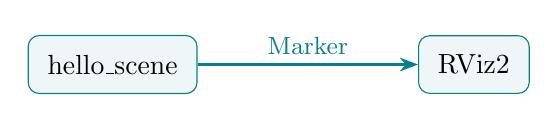
\begin{tikzpicture}[node distance=28mm]
\node[draw=tealblue,fill=pale,rounded corners,inner sep=7pt] (a) {hello\_scene};
\node[draw=tealblue,fill=pale,rounded corners,inner sep=7pt,right=of a] (b) {RViz2};
\draw[-{Stealth},thick,tealblue] (a) -- node[above,font=\small] {Marker} (b);
\end{tikzpicture}
\end{center}
RViz2 显示收到的数据，不负责机器人动力学。本章圆盘是一个静态图形。

\section{确认主机环境}
本课程验证平台是 Ubuntu 26.04 和 ROS 2 Lyrical。已有主机不用重装。打开 bash，先运行：
\begin{lstlisting}[language=bash,numbers=none]
source /opt/ros/lyrical/setup.bash
printenv ROS_DISTRO
ros2 pkg prefix rviz2
colcon version-check --help
\end{lstlisting}
前三项应分别加载环境、输出 lyrical、找到 RViz2。最后一项只是检查 colcon 命令，后文构建才是实际工具链验收。

干净主机应先按
\href{https://github.com/ros2/ros2_documentation/blob/rolling/source/Get-Started/Installation/Ubuntu-Install-Debs.rst}{ROS 官方安装步骤}
配置 UTF-8、Universe 与 ros-apt-source。已配好软件源的 Ubuntu 26.04 可安装
\code{ros-lyrical-desktop}、\code{ros-dev-tools}、\code{libeigen3-dev}。
不要把其他 Ubuntu 版本与 Lyrical 的二进制包混用。

\begin{notebox}
Lyrical 的 ROS 接口按 C++20 编译；本课程独立几何和数学代码采用 C++17。读者不必先学习 concepts 等高级特性。ROS 的 Python 包使用系统 Python，构建时显式指定 \code{/usr/bin/python3}。
\end{notebox}

\section{构建并启动}
以下路径是当前主机仓库位置；换机器后改成自己的路径。每个新终端都要先加载主机环境，再加载课程工作空间。
\begin{lstlisting}[language=bash,numbers=none]
source /opt/ros/lyrical/setup.bash
cd /home/zdp/ForCodex/ros2_motion_planning_course/ros2_ws
colcon build --symlink-install --cmake-args \
  -DCMAKE_BUILD_TYPE=RelWithDebInfo \
  -DPython3_EXECUTABLE=/usr/bin/python3
source install/setup.bash
ros2 launch motion2d_bringup ch01.launch.py
\end{lstlisting}
\code{motion2d} 装算法和节点；\code{motion2d_bringup} 装配置、launch 与 RViz2 视图。
\code{--symlink-install} 方便开发时编辑配置。参数只在启动时读取，所以修改 YAML 后重启节点。

RViz2 应显示浅色背景、0.5 m 网格和原点的青色圆盘，Fixed Frame 为 map。无图形界面可加 \code{rviz:=false}；这不能替代图形验收。

\begin{figure}[htbp]
\centering
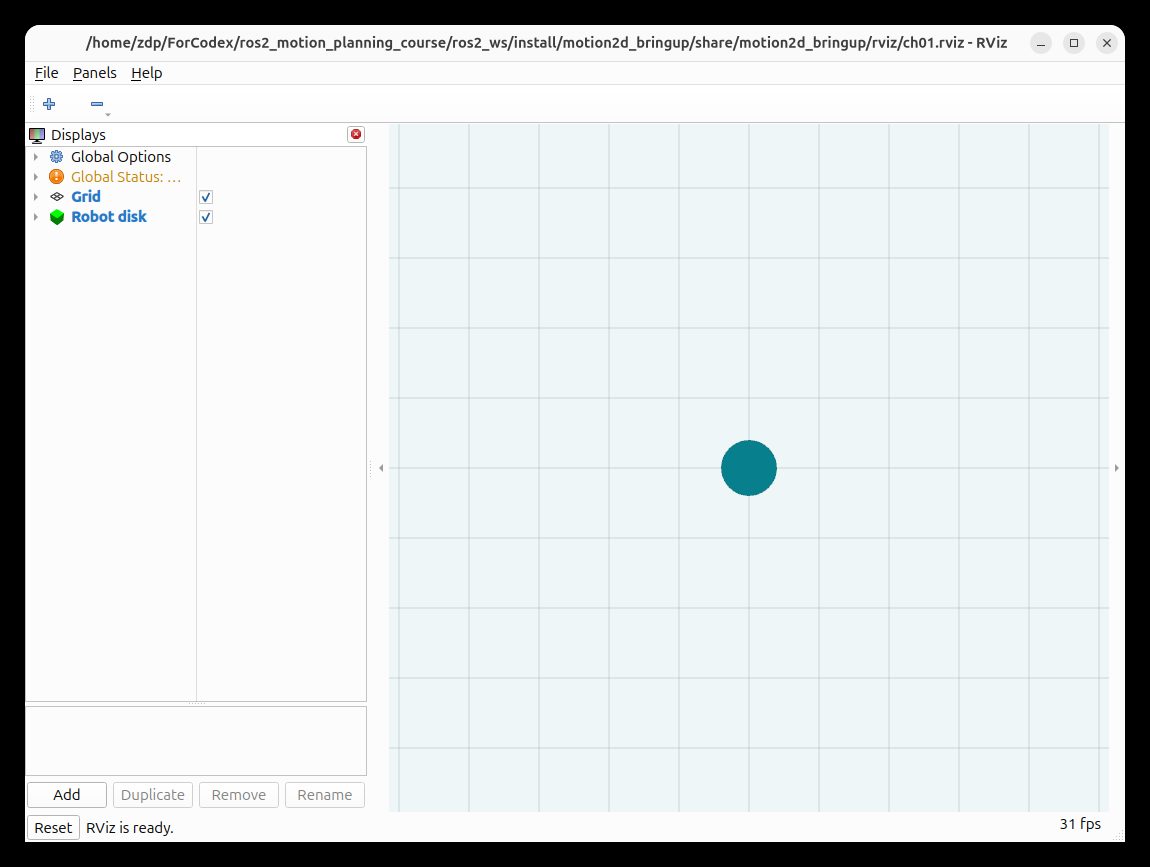
\includegraphics[width=.88\linewidth]{figures/ch01_rviz.png}
\caption{主机实际运行画面。圆盘直径为 0.40 m，小于一个 0.5 m 网格。}
\end{figure}
此时 Global Status 可能提示尚无 TF 数据，因为本章还没有发布坐标树。Marker 已直接在 map 帧中，所以仍可正确显示；下一章建立 TF 后该提示消失。

\section{圆盘为什么用直径？}
用一个很薄的 CYLINDER 表示圆盘。Marker 的 scale 是物体的完整尺寸，因此
\begin{equation}
d_x=d_y=2r,\qquad r=0.20\ \mathrm{m}\ \Rightarrow\ d_x=d_y=0.40\ \mathrm{m}.
\end{equation}
\code{scale.z=0.05} 只是显示厚度，后续平面碰撞只使用半径。单位四元数的 w 分量为 1；alpha 为 0 的图形完全透明。

下面直接读取实际源码的标记区域。修改代码后重新编译本书，摘录会同步更新：
\lstinputlisting[language=C++,linerange={marker_begin-marker_end},
  includerangemarker=false]{../ros2_ws/src/motion2d/src/nodes/hello_scene_node.cpp}

\section{发布一次，为什么晚启动也能看到？}
本节点使用 reliable + transient-local QoS，保留最后一条 Marker。RViz2 订阅同样配置持久性，晚启动时可取到保留的消息。节点退出后，不应假设消息仍会被保留。

第二个终端加载环境，进入工作空间后运行：
\begin{lstlisting}[language=bash,numbers=none]
ros2 topic echo /visualization/robot --once \
  --qos-durability transient_local
/usr/bin/python3 ../scripts/check_ch01.py
\end{lstlisting}
检查程序确实作为晚加入的订阅者接收消息，并核对帧、类型与默认尺寸。此时消息 stamp 用系统时间；下一章再引入仿真时钟。

\clearpage
\section{动手练习与验收}
\begin{enumerate}
\item \textbf{理解：}节点与话题的区别是什么？发布者先启动、RViz2 后启动时，为什么仍能收到圆盘？
\item \textbf{代码：}完成 \code{exercises/ch01/starter/marker_scale.hpp} 中的
\code{EXERCISE(ch01-1)}。检查方法、分级提示和独立参考答案位于同目录。
\item \textbf{实验：}在 \code{ch01.yaml} 中把半径改成 0.35 m、x 改为 1.0 m，重启。先预测消息和网格上的尺寸，再观察；检查默认配置前恢复参数。
\end{enumerate}
应看到直径 0.70 m、圆心 $(1,0)$ 的圆盘。若图形不见了，依次检查 Fixed Frame、话题、alpha 与 QoS。若找不到包，检查是否加载课程的 install 环境。

\subsection*{独立编译练习}
练习的输入是半径，输出是 Marker 的 x/y 尺寸。下面的 starter 故意保留一个需要你修改的返回值；它没有被链接到正式演示中。
\lstinputlisting[language=C++,numbers=none]{../exercises/ch01/starter/marker_scale.hpp}
从仓库根目录运行：
\begin{lstlisting}[language=bash,numbers=none]
g++ -std=c++17 -Wall -Wextra -Iexercises/ch01/starter \
  exercises/ch01/check.cpp -o /tmp/ch01_exercise
/tmp/ch01_exercise
\end{lstlisting}
未完成时检查输出 FAIL；改对后输出 PASS。检查包含两个半径，避免只为一个例子填写常数。若卡住，先看同目录的 hints，再读 solutions 的解释；把编译命令中的 starter 换成 solutions 即可验证参考解。

本章完成后，你应能解释图形由哪个节点发布、消息中哪些量决定尺寸，以及如何让另一个程序接收这条消息。

\chapter{二维坐标、时间与接口}\label{ch:frames}
\begin{notebox}
\textbf{目标}\quad 正确旋转、平移、求逆，并用一个仿真时钟驱动坐标树。\\
\textbf{先修}\quad 第 1 章；二维向量和正弦、余弦。矩阵只需要理解本章的两行乘法。
\end{notebox}

\section{一个点可以有不同坐标}
机器人位于地图坐标 $(1,2)$，朝向正北。雷达观测到正前方 2 m 的点。它在机体系是 $(2,0)$，在地图系是 $(1,4)$。坐标变了，物理上的点没有变。

我们采用右手系：机体 x 轴向前、y 轴向左、z 轴向上，逆时针偏航为正，角度使用弧度。一个平面位姿记作 $T_{A\leftarrow B}=(t,\psi)$：它把 B 系的坐标换成 A 系坐标。

\subsection*{从两根坐标轴得到旋转矩阵}
先想象只旋转一个向量，暂时把两个坐标系原点放在一起。
沿 B 系 x 轴走 1 m，在 A 系中的水平、竖直分量分别为 $\cos\psi,\sin\psi$。
B 系 y 轴比 x 轴多转 $\pi/2$，其分量是 $-\sin\psi,\cos\psi$。
任意点 $p_B=(x_B,y_B)$ 都可看成“沿第一根轴走 $x_B$，再沿第二根轴走 $y_B$”，所以
\begin{align}
x_A-t_x&=x_B\cos\psi-y_B\sin\psi,\\
y_A-t_y&=x_B\sin\psi+y_B\cos\psi.
\end{align}
矩阵只是把这两行计算排在一起：第一列记录旋转后的 x 轴，第二列记录旋转后的 y 轴。
向量默认写成一列，上标 $\top$ 表示把行、列互换。
\begin{equation}
R(\psi)=\begin{bmatrix}\cos\psi&-\sin\psi\\ \sin\psi&\cos\psi\end{bmatrix},
\qquad p_A=R(\psi)p_B+t.
\label{eq:transform}
\end{equation}
先旋转向量，再加上 B 原点在 A 中的位置 t。例子中 $\psi=\pi/2$，
$R(2,0)^\top=(0,2)^\top$，再加 $(1,2)^\top$ 就得到 $(1,4)^\top$。
这个顺序对应两件不同的事：坐标轴改变方向，坐标原点改变位置。

\begin{center}
\begin{tikzpicture}[x=1cm,y=1cm,>=Stealth]
\draw[step=1,linecolor] (0,0) grid (4,4);
\draw[->,muted] (0,0)--(4.5,0) node[right] {$x_{\rm map}$};
\draw[->,muted] (0,0)--(0,4.7) node[above] {$y_{\rm map}$};
% 虚线只延长机体 x 轴，不叠画在实线和箭头上。
\draw[dashed,tealblue] (1,3.25)--(1,4);
\draw[tealblue,thick,->] (1,2)--(1,3.2);
\draw[tealblue,thick,->] (1,2)--(.1,2);
\node[right,tealblue,fill=white,inner sep=2pt] at (1.18,3.25) {$x_{\rm body}$};
\node[left,tealblue] at (-.15,2.3) {$y_{\rm body}$};
% 坐标说明放到网格外，用引线指向对应点。
\draw[muted,thin] (1.12,2.03)--(3.5,2.55)--(4.35,2.55);
\node[right,align=left] at (4.45,2.55) {圆心\\map $(1,2)$};
\draw[muted,thin] (1.12,4.07)--(3.5,4.35)--(4.35,4.35);
\node[right,align=left] at (4.45,4.35)
  {同一个观测点\\map $(1,4)$，body $(2,0)$};
\fill[tealblue] (1,2) circle (2pt);
\fill[navy] (1,4) circle (2pt);
\end{tikzpicture}
\end{center}

\section{从公式到一个小函数}
\code{Pose2D} 只保存一个二维向量和一个角度。几何库不包含 ROS 头文件，可以单独用 C++17 编译、调试和测试。
\lstinputlisting[language=C++,linerange={rotation_begin-rotation_end},
  includerangemarker=false]{../ros2_ws/src/motion2d/src/geometry/se2.cpp}

\paragraph{代码中的每一步}
Matrix2d 表示 $2\times2$ 的数表；逗号初始化依次填写两行。
transformPoint 中的矩阵乘法正是上面的两行标量式，pose.position 就是 t。
可以先在纸上算 $\psi=0$ 和 $\psi=\pi/2$，再单步调试查看四个矩阵元素。
函数所在的 se2 文件名表示平面刚体变换；本章所需运算就是旋转、平移与合成。

\section{逆变换与变换链}
从式 \eqref{eq:transform} 两侧减去 t，再左乘 $R^\top$：
\begin{equation}
p_B=R^\top(p_A-t)=R^\top p_A-R^\top t.
\end{equation}
为什么左乘 $R^\top$ 能消去 R？把矩阵直接相乘：
\begin{equation}
R^\top R=
\begin{bmatrix}
\cos^2\psi+\sin^2\psi&-\cos\psi\sin\psi+\sin\psi\cos\psi\\
-\sin\psi\cos\psi+\cos\psi\sin\psi&\sin^2\psi+\cos^2\psi
\end{bmatrix}=I.
\end{equation}
I 是对角线为1、其余为0的单位矩阵，乘向量后保持原值。
因此逆旋转等于转置，逆位姿为 $(-R^\top t,-\psi)$。
手算例子中，先做 $(1,4)-(1,2)=(0,2)$，再顺时针转 $90^\circ$，就回到 $(2,0)$。

若雷达相对机体有固定外参 $T_{B\leftarrow L}$，机体相对地图为 $T_{M\leftarrow B}$，则
\begin{equation}
T_{M\leftarrow L}=T_{M\leftarrow B}T_{B\leftarrow L}.
\end{equation}
这里的位姿乘号表示“接着做另一个变换”。写出中间点便能展开它：
\begin{align}
p_B&=R_{BL}p_L+t_{BL},\\
p_M&=R_{MB}(R_{BL}p_L+t_{BL})+t_{MB}\\
   &=(R_{MB}R_{BL})p_L+(R_{MB}t_{BL}+t_{MB}).
\end{align}
所以合成的平移为 $R_{MB}t_{BL}+t_{MB}$，朝向为 $\psi_{MB}+\psi_{BL}$。
compose 正是先调用 transformPoint 得到这个平移，再相加朝向。
例如雷达在车体前方0.5 m，车体位于 $(1,2)$ 且朝北，雷达在地图中就位于 $(1,2.5)$。
从右向左读下标，便得到“雷达点→机体点→地图点”的计算顺序。课程默认传感器位于圆心，外参为单位变换；保留显式外参能让后续实验改变安装位置。

\section{运行与理解数值误差}
按第 1 章的方法重新构建、加载环境，在工作空间运行：
\begin{lstlisting}[language=bash,numbers=none]
ros2 run motion2d se2_demo
colcon test --packages-select motion2d \
  --event-handlers console_direct+
colcon test-result --verbose
\end{lstlisting}
示例输出机体点 $(2,0)$、地图点 $(1,4)$，再恢复到 $(2,0)$。
浮点运算中的 $\cos(\pi/2)$ 可能是接近零的小数，所以比较使用绝对误差容限 $10^{-12}$，不是要求每个计算结果逐位相同。

角度是另一个边界问题。$179^\circ$ 到 $-179^\circ$ 的最短旋转只有 $2^\circ$。先将差值归一到 $[-\pi,\pi)$，再把它作为误差。函数 \code{wrapAngle} 使用弧度；输入 90 表示 90 rad，不是 90 度。

\section{练习：自己写一次逆变换}
\begin{enumerate}
\item \textbf{推导：}为何逆变换中不能只把 t 取负？用 $\psi=90^\circ,t=(1,2)$ 给一个反例。
\item \textbf{代码：}补完 \path{exercises/ch02/starter/inverse_point.hpp} 的标记函数。它复用正式库的 \code{Pose2D}，检查包括两个旋转方向。
\item \textbf{实验：}把示例朝向换成 $-90^\circ$，预测地图点，再运行核对。还可以将激光外参设为机体前方 0.5 m，手算其地图位置。
\end{enumerate}
独立编译命令、分级提示和参考答案位于同章习题 README。用正向变换再逆变换的往返结果检查自己：应回到原来的点，差别只剩浮点舍入误差。

\section{仿真时间与真实等待时间}
假设每个仿真步长是 $\Delta t=0.005$ s。第 k 步的仿真时间为
\begin{equation}
t_k=k\Delta t.
\end{equation}
即使电脑偶尔调度得慢，状态仍然只前进一个固定步长。例如电脑用0.008 s才完成一次计算，模拟时刻仍从0.005 s增加到0.010 s；
真实等待时间决定程序跑得快慢，仿真时间决定方程积分了多久。

\code{SimClock} 用整数 tick 和整数纳秒保存时间，避免反复执行浮点加法。暂停时自动 advance 返回 false，单步只在暂停时允许执行：
\par\noindent\begin{minipage}{\linewidth}
\lstinputlisting[language=C++,linerange={clock_begin-clock_end},
  includerangemarker=false]{../ros2_ws/src/motion2d/src/sim/sim_clock.cpp}
\end{minipage}\par
本章由 \code{frame_demo_node} 唯一发布 \code{/clock}；RViz2 和节点都设置 \code{use_sim_time=true}。
暂停后重复发送当前时间，便于新订阅者获得它。判断是否发生新的一步，应比较时间值，而不是数消息。
例如收到0.010、0.010、0.015 s三条消息，物理状态只从第2步推进到第3步。

\section{把坐标放到 ROS 的 TF 树中}
\[
\texttt{map}\to\texttt{odom}\to\texttt{base\_link}
\to\{\texttt{laser},\texttt{imu\_link}\}.
\]
本章 map 到 odom 为单位变换；传感器位于圆心、与机体系对齐，也是单位变换。这三条静态边通过 \code{/tf_static} 发布。odom 到 base\_link 是带采样时刻的动态边，通过 \code{/tf} 发布。

为观察旋转效果，示例固定圆心 $(1,2)$，采用解析朝向
\begin{equation}
\psi(t)=\frac{\pi}{2}+0.2t.
\end{equation}
角速度由求导得到 $\dot\psi=0.2$ rad/s。圆心固定、坐标轴匀速转动，
因此图中的蓝色箭头能清楚展示同一个 laser 系向量怎样在地图中转动。

\subsection*{消息里为什么出现半角？}
ROS 用四个数表示空间朝向。本课程只有绕 z 轴的平面旋转，令 $q_x=q_y=0$。
接口的平面旋转关系为
\begin{equation}
R_q=\begin{bmatrix}1-2q_z^2&-2q_zq_w\\2q_zq_w&1-2q_z^2\end{bmatrix},
\qquad q_z^2+q_w^2=1.
\end{equation}
用一个角 $\theta$ 参数化单位圆：$q_z=\sin\theta,q_w=\cos\theta$。
双角公式给出 $1-2\sin^2\theta=\cos2\theta$、$2\sin\theta\cos\theta=\sin2\theta$，
因此 $R_q=R(2\theta)$。为了表示 yaw=$\psi$，应取 $\theta=\psi/2$：
\begin{equation}
(q_x,q_y,q_z,q_w)=(0,0,\sin(\psi/2),\cos(\psi/2)).
\end{equation}
例如 $90^\circ$ 对应 $q_z=q_w=\sqrt2/2$；零角对应 $(0,0,0,1)$。
这也解释了第一章为什么把 w 设为1：它满足单位长度并表示零旋转。
发布时刻直接取仿真时钟，不能换成回调到达的真实时间：
\par\noindent\begin{minipage}{\linewidth}
\lstinputlisting[language=C++,linerange={frame_begin-frame_end},
  includerangemarker=false]{../ros2_ws/src/motion2d/src/nodes/frame_demo_node.cpp}
\end{minipage}\par

\section{暂停、单步与重置实验}
停止第 1 章程序，重新构建并加载环境后启动：
\begin{lstlisting}[language=bash,numbers=none]
ros2 launch motion2d_bringup ch02.launch.py
\end{lstlisting}
另一个终端同样加载环境后调用：
\begin{lstlisting}[language=bash,numbers=none]
ros2 service call /sim/pause std_srvs/srv/SetBool "{data: true}"
ros2 service call /sim/step std_srvs/srv/Trigger "{}"
ros2 service call /sim/reset std_srvs/srv/Trigger "{}"
ros2 service call /sim/pause std_srvs/srv/SetBool "{data: false}"
\end{lstlisting}
暂停时圆盘朝向和箭头冻结；每次单步前进 5 ms；reset 回到时间零、初始朝向，并保持暂停。单步服务在暂停状态使用，方便逐次观察积分结果。

在工作空间运行 \code{/usr/bin/python3 ../scripts/check_ch02.py} 可检查唯一 TF 父帧、解析朝向、冻结时钟、5 ms 单步、reset 和恢复运行。它会改变演示状态，仅用于本章实验。

\begin{notebox}
重置会使仿真时间向后跳，TF 监听器会清空缓存，这是新试验的正常边界。本节点每隔 1 s 墙钟时间重发静态外参，暂停时同时重发当前动态边，使监听器能在 reset 后重新获得坐标关系。
后续估计器也会在这个时刻开始新的积分历史。
\end{notebox}

\begin{figure}[htbp]
\centering
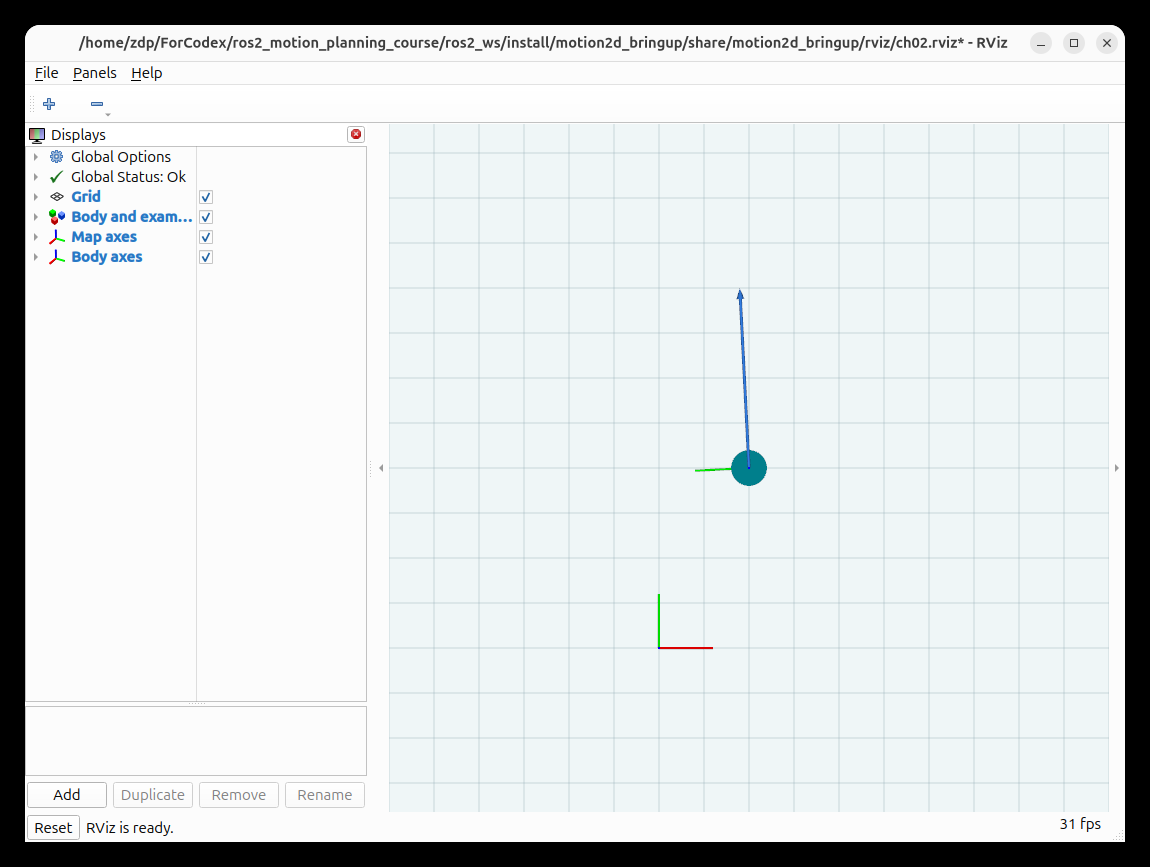
\includegraphics[width=.65\linewidth]{figures/ch02_rviz.png}
\caption{圆心保持在 $(1,2)$，蓝色观测向量随机体坐标系转动；地图坐标轴保持不动。}
\end{figure}

\subsection*{时间练习}
先暂停，再连续调用 step 十次，预测仿真时间增量和朝向增量，之后查看 \code{/clock} 和 TF 核对。标准答案是 0.05 s 与 0.01 rad。改变 YAML 中的 dt 后要重新推导；不应继续照搬默认值的检查脚本。


\chapter{一个可复现的二维世界}\label{ch:world}
\begin{notebox}
\textbf{目标}\quad 生成随机圆与凸多边形，显示起终点，检查有半径的机器人能否放入世界。\\
\textbf{先修}\quad 前两章；向量点积。凸包与距离的必要直觉在本章说明。
\end{notebox}

\section{先看世界，再谈算法}
停止之前的演示，重新构建并加载工作空间后运行：
\begin{lstlisting}[language=bash,numbers=none]
ros2 launch motion2d_bringup ch03.launch.py
\end{lstlisting}
默认世界宽、高都是 20 m，边界以原点为中心。seed=42 时生成 8 个圆和 8 个凸多边形；机器人在 $(-8,-8)$，目标在 $(8,8)$。世界是静态的，机器人尚未运动。

此处显示的是仿真掌握的完整几何。后续激光只能看见无遮挡且在量程内的表面，建图不能直接读取这些障碍物顶点。理解这个数据边界，才能公平比较真值模式和 SLAM 模式。

\begin{figure}[ht]
\centering
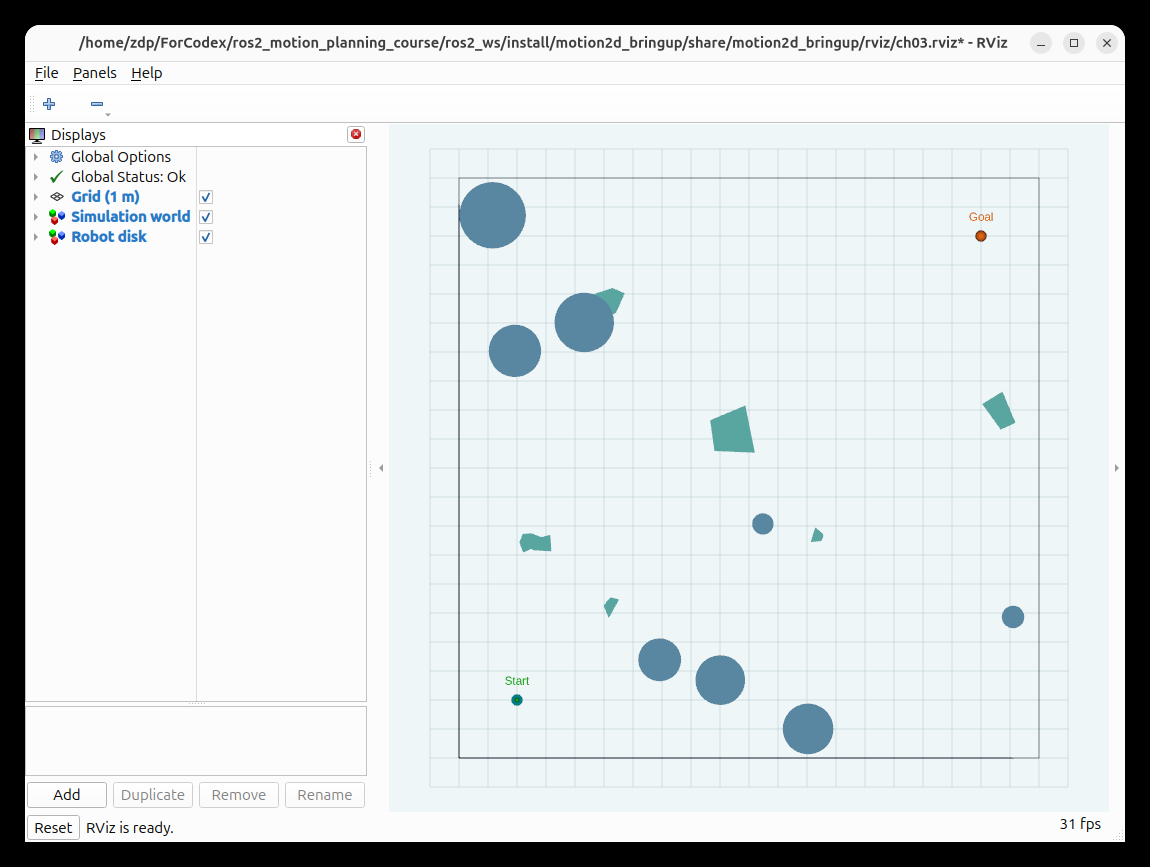
\includegraphics[width=.85\linewidth]{figures/ch03_rviz.png}
\caption{seed=42 的实际世界。圆和凸多边形可以重叠；Start 与 Goal 分别标出起终点。}
\end{figure}

\clearpage
\section{圆心不碰撞，不代表圆盘不碰撞}
半径为 r 的圆盘中心位于 p，圆形障碍中心为 c、半径为 R。两者相切时，中心距为 $r+R$，本课程把接触计为碰撞：
\begin{equation}
\|p-c\|>r+R \quad\Longleftrightarrow\quad \text{与该障碍无碰撞}.
\end{equation}
定义单个障碍的有符号距离 $d(p)$：外部为正、内部为负。自由区域中，圆盘需要 $d(p)>r$。如要额外留出安全裕量 $\delta$，使用 $d(p)>r+\delta$；物理半径与规划裕量是两个不同参数。

世界边界也限制可用空间。核心函数在自由域中取边界和所有障碍的最小距离，再比较半径：
\par\noindent\begin{minipage}{\linewidth}
\lstinputlisting[language=C++,linerange={clearance_begin-clearance_end},
  includerangemarker=false]{../ros2_ws/src/motion2d/src/sim/world.cpp}
\end{minipage}\par
占据区或越界时，这个函数用于判断符号，不承诺给出并集内部的精确 ESDF；第 12 章会专门构建距离场。

\section{点到线段的距离}
多边形边界由线段组成。设边为 $a\to b$，把点 p 投影到直线上：
\begin{equation}
t^*=\frac{(p-a)^\top(b-a)}{\|b-a\|^2},\qquad
t=\min(1,\max(0,t^*)),\qquad q=a+t(b-a).
\end{equation}
q 是线段上离 p 最近的点，距离是 $\|p-q\|$。限制 t 很重要：离线段延长线很近，不代表离有限线段很近。若 a=b，则线段退化为一个点。
\par\noindent\begin{minipage}{\linewidth}
\lstinputlisting[language=C++,linerange={distance_begin-distance_end},
  includerangemarker=false]{../ros2_ws/src/motion2d/src/geometry/obstacles.cpp}
\end{minipage}\par
对逆时针凸多边形，内部点位于每条有向边的左侧。若点在内部，距离取负；外部则取到全部边的最小距离。

\section{随机多边形为什么从凸包开始？}
随意把随机点连起来可能产生自交。我们的步骤是：在一个采样圆盘内生成点，再取凸包。可把凸包想成绕所有点拉紧的橡皮筋。实现先按 x/y 排序，再维护上、下两条只向同一方向拐弯的链。

若 $u,v$ 独立服从 $[0,1)$ 均匀分布，使用
\begin{equation}
\theta=2\pi u,\qquad \rho=R\sqrt v,\qquad
p=c+\rho(\cos\theta,\sin\theta)
\end{equation}
让采样点在圆盘面积上均匀。因为半径不超过 $\rho$ 的面积比例是 $\rho^2/R^2$，所以半径要取平方根。

代码中 \code{polygon_samples=8} 表示采样八个点，凸包顶点通常更少。校验要求顶点有限、严格凸、逆时针；对每条边检查其余顶点都位于左侧，也能排除自交星形。

不同障碍可以重叠，这仍是合法障碍并集。世界生成器只拒绝无效形状、越界和侵入起终点保护圆的候选。每个形状最多尝试 1000 次，失败明确报告，不偷偷换种子。

\section{先检查可达，再讲最短路径}
起点、终点各自无碰撞，并不意味着中间一定连通。我们先用粗网格和四邻接 flood fill 检查连通性：从起点所在格入队，反复访问相邻自由格，能到终点格即通过。它不寻找最短路径，也不替代第 11 章的 A*。

不能仅检查格中心。对于宽 $\Delta x$、高 $\Delta y$ 的单元，中心到最远角点的距离为
\begin{equation}
\epsilon_{\rm cell}=\frac12\sqrt{\Delta x^2+\Delta y^2}.
\end{equation}
中心只有在净空大于 $r+\delta+\epsilon_{\rm cell}$ 时才标为自由。这保证整个单元能容纳圆盘，代价是窄通道可能被保守拒绝。

默认检查分辨率 0.25 m。若失败，可以明确减小分辨率或关闭 \code{require_connected} 观察场景；同一个 seed 不会自动被替换成“更好看”的世界。记录失败案例也是学习的一部分。

\clearpage
\section{参数、练习与验收}
编辑 \path{ros2_ws/src/motion2d_bringup/config/ch03.yaml} 后重启。公共 x/y/radius 同时提供给坐标节点和世界节点；圆盘显示与碰撞不应使用两套不同半径。
\begin{enumerate}
\item \textbf{理解：}给一个圆心在自由空间、圆盘却碰撞的例子。解释相切和安全裕量。
\item \textbf{代码：}实现 \path{exercises/ch03/starter/segment_distance.hpp} 的点线段距离。独立检查覆盖内点、端点外、线段上和退化线段；提示与参考解单独存放。
\item \textbf{实验：}相同配置和 seed=42 启动两次，比较地图。然后改为 43，再把两类障碍各增至 20 个，记录可达性和起终点净空。
\end{enumerate}
代码练习从仓库根目录单独编译，不依赖 ROS：
\begin{lstlisting}[language=bash,numbers=none]
g++ -std=c++17 -I/usr/include/eigen3 \
  -Iexercises/ch03/starter \
  exercises/ch03/check.cpp -o /tmp/ch03_exercise
/tmp/ch03_exercise
\end{lstlisting}
将 starter 替换为 solutions 可以检验参考解。先运行未完成的练习观察失败位置，再修改投影公式；不要通过删掉检查来得到“通过”。

在同一标准库和参数下，固定种子复现相同世界；跨编译器标准库版本不保证分布函数的逐位一致。输出状态说明是否执行了连通性检查，避免把“没有检查”当成“已经通过”。

运行 \code{colcon test} 检查几何、碰撞和可达性；演示运行时，在工作空间执行以下命令核对默认消息：
\begin{lstlisting}[language=bash,numbers=none]
/usr/bin/python3 ../scripts/check_ch03.py
\end{lstlisting}
RViz2 展示全部障碍、边界和起终点，图形并非激光建图结果。

\begin{notebox}
\textbf{常见问题}

看不见障碍时，先确认 Fixed Frame 为 map、World 的话题为
\code{/visualization/world}，再检查节点有没有因无效参数退出。改参数后要重启；
本章尚不提供运行中重建世界。若可达性检查失败，保留 seed 和配置，再研究分辨率与通道宽度。
\end{notebox}

\chapter{让圆盘运动：位置、速度与力}\label{ch:robot}
\begin{notebox}
\textbf{目标}\quad 区分理想位置执行与物理运动；让碰撞半径真正约束移动。\\
\textbf{先修}\quad 前三章、速度与加速度的含义。先运行，再推导。
\end{notebox}

\section{圆心状态与圆盘外形}
机器人用圆心描述状态，圆盘描述占据的空间：
\begin{equation}
x=(p,v,\psi,\omega),\qquad
p=(p_x,p_y),\quad v=(v_x,v_y).
\end{equation}
位置单位 m，速度 m/s，yaw 为 rad，角速度 rad/s。位置和速度在 odom 系表达；
本章的 map 与 odom 重合。半径 r 单独参与碰撞，不把“质点状态”误解为“没有体积”。
若 r=0，才是几何质点；屏幕上的小点仅用于看清位置。

控制量不同，模型的物理意义就不同。理想到点输入目标位姿；速度模型输入平面速度；
惯性模型输入力和偏航力矩。它们分别使用不同话题，不能把同一个数值悄悄解释成另一种单位。
先完成最容易运行的理想到点，再逐项加入连续运动模型。

\section{先让机器人到一个点}
停止之前的场景，重新构建并加载 install 后运行：
\begin{lstlisting}[language=bash,numbers=none]
ros2 launch motion2d_bringup ch04.launch.py model:=ideal
\end{lstlisting}
在 RViz2 用 2D Goal Pose 工具点击、拖动，指定目标位置和 yaw。工具向
\code{/command/pose} 发布消息。也可在第二个已加载 ROS 环境的终端发送：
\begin{lstlisting}[language=bash,numbers=none]
ros2 topic pub --once /command/pose geometry_msgs/msg/PoseStamped \
  "{header: {frame_id: odom}, pose: {position: {x: -7.0, y: -8.0}, orientation: {w: 1.0}}}"
\end{lstlisting}
默认从 $(-8,-8)$ 移到 $(-7,-8)$，图中留下接受过的运动轨迹。目标在下一 tick 才执行；
暂停时发目标，圆盘保持不动，单步后才到达目标。

\clearpage
\section{扫过的空间也要安全}
起终点安全并不足够。半径 r 的圆盘沿线段 $[p_0,p_1]$ 移动，扫过的区域是胶囊形。
对于圆心 c、半径 R 的障碍，无碰撞要求
\begin{equation}
\operatorname{dist}(c,[p_0,p_1])>R+r.
\end{equation}
这里直接复用第 03 章的点线段距离。对凸多边形，检查起终点和运动线段到每条边的距离；
对矩形边界，内缩后的矩形是凸集，检查两个端点即可保证整条直线留在其中。

\begin{center}
\begin{tikzpicture}[x=1cm,y=1cm]
\fill[tealblue!12,rounded corners=8mm] (-3,-.45) rectangle (3,.45);
\draw[tealblue,dashed,rounded corners=8mm] (-3,-.45) rectangle (3,.45);
\draw[-{Stealth},thick,navy] (-2.55,0) -- (2.55,0);
\draw[fill=white,tealblue,thick] (-2.55,0) circle (.45);
\draw[fill=white,tealblue,thick] (2.55,0) circle (.45);
\draw[fill=muted!50,navy] (0,.15) circle (.55);
\node[below] at (-2.55,-.5) {$p_0$};
\node[below] at (2.55,-.5) {$p_1$};
\node[above] at (0,.8) {端点自由，整段被挡住};
\end{tikzpicture}
\end{center}

\par\noindent\begin{minipage}{\linewidth}
\lstinputlisting[language=C++,linerange={sweep_begin-sweep_end},
  includerangemarker=false]{../ros2_ws/src/motion2d/src/sim/swept_collision.cpp}
\end{minipage}\par
代码没有按固定间距抽样，因此不会因为障碍很薄、目标很远，就从障碍另一侧“穿过去”。
这是连续直线扫掠的几何检查，浮点实现仍受数值精度限制。

\clearpage
\section{理想到点不产生真实 IMU}
通过几何检查后，理想模型直接赋值目标位姿：
\par\noindent\begin{minipage}{\linewidth}
\lstinputlisting[language=C++,linerange={ideal_begin-ideal_end},
  includerangemarker=false]{../ros2_ws/src/motion2d/src/sim/ideal_model.cpp}
\end{minipage}\par
位置在一个 tick 中改变，不代表机器人以一个有限速度完成了运动。速度和加速度字段为
未使用的零值；不能对这种跳变做差分，再把结果称为模拟 IMU。平滑轨迹执行将在轨迹章节加入。

\begin{figure}[ht]
\centering
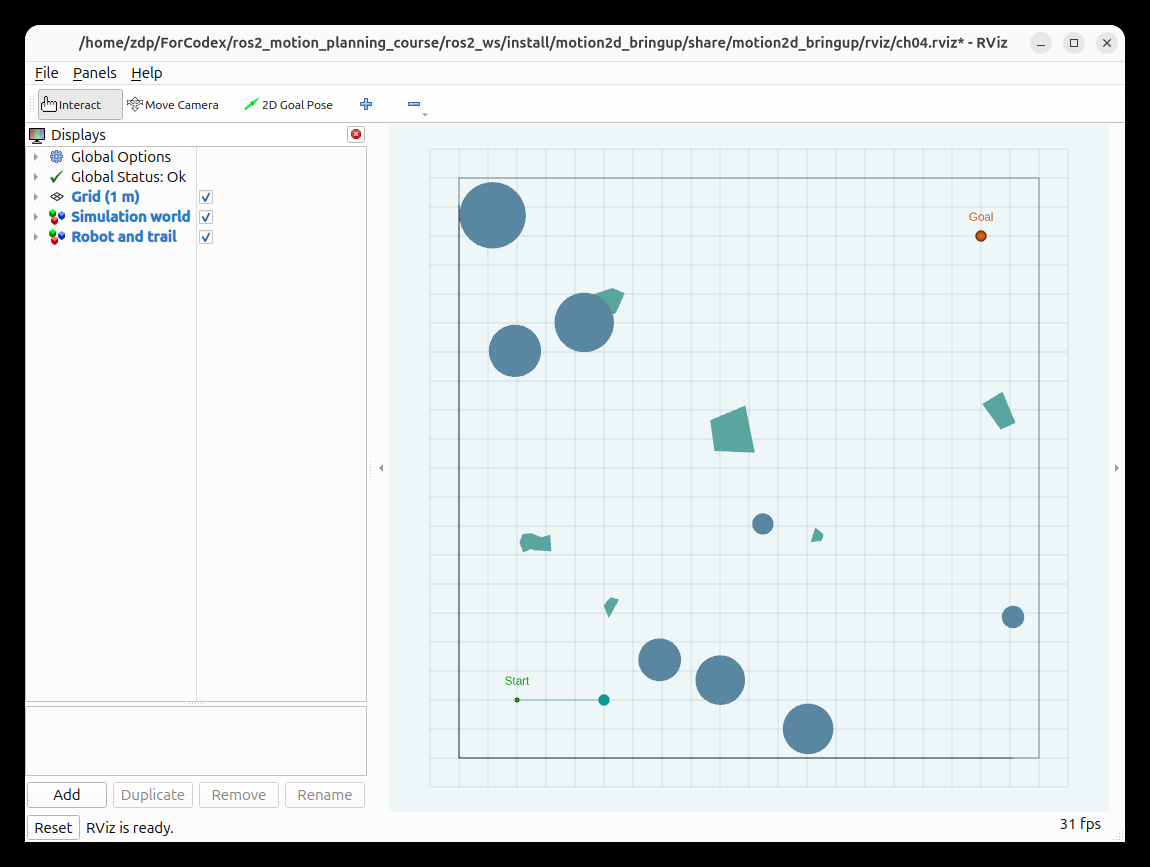
\includegraphics[width=.78\linewidth]{figures/ch04_ideal_rviz.png}
\caption{实际 RViz2 画面：世界、圆盘与已接受的移动轨迹。}
\end{figure}

\section{冻结试验与重新开始}
若扫掠检查失败，程序不接受候选状态：位置、速度和时间停在上一个通过检查的 tick，
\code{/sim/status} 为 \code{collision_predicted}，圆盘变红。
这是提前终止试验，尚未模拟接触力、反弹或摩擦。它没有把撞入障碍的状态推回自由空间。
需要调用 reset 才能继续。

\begin{lstlisting}[language=bash,numbers=none]
ros2 service call /sim/reset std_srvs/srv/Trigger "{}"
ros2 service call /sim/step std_srvs/srv/Trigger "{}"
ros2 service call /sim/pause std_srvs/srv/SetBool "{data: false}"
\end{lstlisting}
reset 开始新试验：回初始状态、清空待执行命令与轨迹、仿真时间归零并暂停。
单步推进一个 dt；恢复运行不改变 dt。墙钟定时器决定运行快慢，整数 tick 决定模拟时间。

% extension_sections
\clearpage
\section{接口、练习与验收}
本章默认 dt=0.005 s。位姿输入接受 odom/map；map 可用是因为本章二者重合。
姿态必须是平面单位四元数，不能把四个分量全填零。时间戳为零表示下一 tick；
非零时间戳只接受当前模拟时刻附近的命令，过旧或过远的未来命令被拒绝。

\code{/sim/pose}、\code{/sim/velocity}、\code{/sim/acceleration} 都是真值调试输出，
平移分量在 odom 系。第 07 章才引入规范的里程计消息与选源，
后续 SLAM 不得读取这些调试话题。本章没有激光或 IMU。

\begin{enumerate}
\item \textbf{理解：}给一个起终点都自由但中间碰撞的例子。为什么瞬时位置赋值不适合 IMU？
\item \textbf{代码 ch04-1：}完成 \path{exercises/ch04/starter/sweep_circle.hpp}。
复用点线段距离，判定圆盘与圆障碍的整段扫掠；相切必须判为碰撞。
\item \textbf{实验：}暂停后发目标并单步；改变半径重复同一条贴近障碍的移动。
记录 seed、半径、起终点和结果。不要把显示尺寸当作碰撞半径。
\end{enumerate}

从仓库根目录编译练习：
\begin{lstlisting}[language=bash,numbers=none]
g++ -std=c++17 -I/usr/include/eigen3 \
  -Iros2_ws/src/motion2d/include -Iexercises/ch04/starter \
  exercises/ch04/check_sweep.cpp \
  ros2_ws/src/motion2d/src/geometry/obstacles.cpp \
  -o /tmp/ch04_sweep
/tmp/ch04_sweep
\end{lstlisting}
提示和参考解分开存放；将 starter 替换为 solutions 可以验证参考解。
演示运行时，从工作空间执行：
\begin{lstlisting}[language=bash,numbers=none]
/usr/bin/python3 ../scripts/check_ch04.py
\end{lstlisting}
脚本会改变场景状态，检查暂停命令、单步、错误帧、碰撞冻结与 reset。
算法测试另外覆盖薄墙和零半径质点。

\begin{notebox}
\textbf{没有移动时先检查}\quad 是否暂停、是否需要 reset、模型是否与输入话题对应，
再检查 frame 和四元数。只运行一个课程 launch，避免多个时钟或 TF 发布者。
\end{notebox}

\chapter{一束光到一圈扫描：CPU 激光雷达}\label{ch:lidar}
\begin{notebox}
\textbf{目标}\quad 用可手算的几何求交构建激光雷达，理解遮挡、角分辨率与测距误差。\\
\textbf{先修}\quad 二维向量、圆方程，以及前四章的坐标、世界与机器人模型。
\end{notebox}

\section{先让一束光碰到障碍}
雷达安装在圆盘中心，发出一条没有宽度的射线。机器人位置与 yaw 决定射线的起点和方向。
雷达不检测机器人自身，否则从圆心发出的光总会先碰到自己的外壳。机器人半径仍参与运动碰撞。

射线用起点 o、单位方向 d 和非负距离 t 表示：
\begin{equation}
p(t)=o+td,\qquad \|d\|=1,\quad t\geq0.
\end{equation}
只有方向已归一化时，t 才直接表示米。测距求的是最近表面，不是障碍中心的距离。
沿同一方向有多个交点时，较近表面会挡住较远表面。

\begin{center}
\begin{tikzpicture}[x=1cm,y=1cm]
\draw[fill=tealblue!15,draw=tealblue,thick] (3,0) circle (1);
\draw[navy,very thick] (5,-1.3)--(5,1.3);
\draw[-{Stealth},navy,thick] (0,0)--(2,0);
\draw[dashed,muted] (2,0)--(5,0);
\fill[navy] (0,0) circle (.05) node[below] {$o$};
\fill[tealblue] (2,0) circle (.06) node[above left] {最近命中};
\fill[navy] (3,0) circle (.04) node[above] {$c$};
\node[above] at (5,1.3) {被遮挡的墙};
\node[below] at (1,-.35) {$t=2$ m};
\end{tikzpicture}
\end{center}

重新构建工作空间并加载 install，先运行不依赖 ROS 回调的几何演示：
\begin{lstlisting}[language=bash,numbers=none]
ros2 run motion2d raycast_demo
\end{lstlisting}
三个距离应依次为 2、4、2 m。前两个分别是圆和墙的单独求交；最后一个在世界中取最近值。
代码位于 \path{src/examples/raycast_demo.cpp}，这里的墙和圆都可以手算。

\clearpage
\section{射线与圆：别忘了第二个根}
把射线代入圆心 c、半径 R 的圆方程，令 $q=c-o$、$h=q^\top d$：
\begin{equation}
\|o+td-c\|^2=R^2
\ \Longrightarrow\ t^2-2ht+\|q\|^2-R^2=0.
\end{equation}
二维叉积 $a\times b=a_xb_y-a_yb_x$ 是一个标量。
单位方向下，$|d\times q|$ 是圆心到射线所在直线的距离，因此
\begin{equation}
D=R^2-(d\times q)^2,\qquad t_\pm=h\pm\sqrt D.
\end{equation}
$D<0$ 时没有交点；$D=0$ 时相切，也算命中。先检查较小的根 $t_-$ 是否非负，
否则再检查 $t_+$。两个根都负，说明圆在射线背后。圆内起点的小根为负，大根是出口；
这有助于测试函数，但课程中的机器人应始终位于自由空间。

\par\noindent\begin{minipage}{\linewidth}
\lstinputlisting[language=C++,linerange={ray_circle_begin-ray_circle_end},
  includerangemarker=false]{../ros2_ws/src/motion2d/src/sim/raycast.cpp}
\end{minipage}\par

没有命中返回正无穷，它与后续所有距离取最小值时自然不起作用。此处先计算真实几何，
量程与测量噪声留给扫描层处理；不要在这个函数里混入 ROS 消息。

\textbf{代码练习 ch05-1：}在 \path{exercises/ch05/starter/forward_root.hpp}
补完根的选择。从仓库根目录运行：
\begin{lstlisting}[language=bash,numbers=none]
g++ -std=c++17 -Iexercises/ch05/starter \
  exercises/ch05/check_root.cpp -o /tmp/ch05_root
/tmp/ch05_root
\end{lstlisting}
先手算圆心 (3,0)、半径 1、起点 (0,0)、方向 (1,0) 的两个根；再把起点放到圆心。
这两个例子分别检查最近回波和第二个根。

\clearpage
\section{射线与线段：平行不一定没交点}
令线段端点为 a、b，$e=b-a$。联立 $o+td=a+ue$，分别取叉积可得
\begin{equation}
t=\frac{(a-o)\times e}{d\times e},\qquad
u=\frac{(a-o)\times d}{d\times e}.
\end{equation}
只有 $t\geq0$ 且 $0\leq u\leq1$ 才命中线段，而不只是命中它所在的直线。
当分母接近零时不能继续做除法：平行但不共线则无交点；共线时将端点投影到射线上，
检查投影区间是否与 $[0,+\infty)$ 相交，取重叠部分的最近点。

\par\noindent\begin{minipage}{\linewidth}
\lstinputlisting[language=C++,linerange={ray_segment_begin-ray_segment_end},
  includerangemarker=false]{../ros2_ws/src/motion2d/src/sim/raycast.cpp}
\end{minipage}\par

世界求交 \code{raycastWorld} 遍历所有圆、所有多边形边，以及矩形边界的四条边，
对得到的非负距离取最小值。这样自然处理遮挡，不依赖障碍物存储顺序。
算法复杂度随表面数线性增长；先保留这个清楚的 CPU 基准，后续再讨论加速。

\textbf{验收与实验：}运行 \code{colcon test --packages-select motion2d}。
几何测试覆盖圆相切、背向、线段端点、平行与共线、矩形角点、遮挡和刚体变换不变性。
把演示的圆移到墙后，预测最近命中；反转射线方向，解释距离为何改变。

\begin{notebox}
这里的浮点容差面向课程的米制小场景。它用于避免接近平行时除以极小数，
不是任意坐标尺度下的精确几何谓词。无效几何应在世界生成边界拒绝。
\end{notebox}

\chapter{机器人感觉到什么：IMU 与传感器时间}\label{ch:imu}
\begin{notebox}
\textbf{目标}\quad 从运动真值产生原始 IMU，区分比力、白噪声和采样时间。\\
\textbf{先修}\quad 第二章的坐标变换、第四章的连续运动，以及第五章的传感器消息。
\end{notebox}

\section{静止的加速度计为什么不为零}
把一个加速度计平放在桌上，它的 z 轴向上时会测到约 $+9.81\ \mathrm{m/s^2}$。
这不是机器人正在加速上升，而是桌面的支持力产生了比力。自由落体才接近零比力；
本课程机器人受平面约束，不模拟自由落体。

设 $R$ 将机体系向量转到世界系，$a$ 是圆心的世界运动加速度，$g$ 是世界重力：
\begin{equation}
f=R^\top(a-g),\qquad g=(0,0,-g_0)^\top,\qquad g_0=9.81\ \mathrm{m/s^2}.
\end{equation}
后续估计器若要恢复运动加速度，需要 $a=Rf+g$，并且必须使用自己的姿态估计。
仿真器内部可用真值 yaw 生成测量，估计器不能把它当作 IMU 给出的姿态。

\begin{center}
\begin{tikzpicture}[>=Stealth]
\draw[thick,navy] (-2,0)--(2,0) node[right] {水平支撑面};
\draw[fill=tealblue!15,draw=tealblue,thick] (-.6,0) rectangle (.6,.45);
\draw[->,thick,tealblue] (0,.45)--(0,1.65) node[above] {$f_z=+g_0$};
\draw[->,thick,navy] (1.1,.3)--(1.1,-1) node[below] {$g_z=-g_0$};
\node[left] at (-.6,.25) {圆盘中心};
\end{tikzpicture}
\end{center}

本章 IMU 在圆心，与 \code{base_link} 同向。机器人只做水平平移和 yaw 转动，
因此 $a_z=0$、roll=pitch=0。陀螺仪理想输出 $(0,0,\dot\psi)$，单位 rad/s，
加速度计理想输出的单位是 $\mathrm{m/s^2}$，不是 g 的倍数。
这一约定参考 \href{https://github.com/ros-infrastructure/rep/blob/master/rep-0145.rst}{REP-145 的 IMU 报告约定（草案）}。

\clearpage
\section{用三行公式读懂理想 IMU}
二维部分只需要一个旋转转置：
\begin{equation}
\begin{bmatrix}f_x\\f_y\end{bmatrix}
=\begin{bmatrix}\cos\psi&\sin\psi\\-\sin\psi&\cos\psi\end{bmatrix}
\begin{bmatrix}a_x\\a_y\end{bmatrix},
\qquad f_z=g_0,\quad \omega_z=\dot\psi .
\end{equation}
例如 yaw 为 $90^\circ$、世界加速度为 $(2,0)$ 时，
世界的 +x 方向正好是机体的 -y，故 $f=(0,-2,9.81)$。

\lstinputlisting[language=C++,linerange={imu_ideal_begin-imu_ideal_end},
  includerangemarker=false]{../ros2_ws/src/motion2d/src/sim/imu.cpp}

\code{ImuSample} 只保存角速度与比力两个三维向量，算法不依赖 ROS。
输入的 \code{acceleration} 成员由动力学或解析轨迹提供；
不要用含噪位置二阶差分代替它。

\textbf{运动模型的选择。}第四章的 \code{reference} 提供一致的解析位置、速度和加速度；
\code{inertial} 从力、质量和阻力计算加速度。二者适合本章。
\code{ideal} 瞬移没有物理导数，\code{velocity} 的速度突变需要脉冲加速度，
都不能据此伪造可融合的 IMU。

\textbf{安装位置的意义。}圆心原地自转时，圆心不产生向心加速度。
圆心本身沿圆轨迹移动时则有。若以后把 IMU 安装到偏离圆心的位置，
需要加入角速度和角加速度引起的杆臂项；本章不暗中模拟这些项。

\begin{notebox}
加速度计不能区分静止和匀速直线运动；两者的运动加速度都是零。
原始 IMU 也不直接测量位置、速度或绝对 yaw。
\end{notebox}

\clearpage
\section{先手算，再运行五个场景}
重新构建工作空间、加载 install 后运行：
\begin{lstlisting}[language=bash,numbers=none]
ros2 run motion2d imu_demo
colcon test --packages-select motion2d
colcon test-result --verbose
\end{lstlisting}
演示的 CSV 输出可与下表核对。角速度单位 rad/s，比力单位 $\mathrm{m/s^2}$。
\begin{center}
\begin{tabular}{lrrrr}
\toprule
场景 & $\omega_z$ & $f_x$ & $f_y$ & $f_z$\\
\midrule
静止 & 0 & 0 & 0 & 9.81\\
匀速 $(2,-1)$ m/s & 0 & 0 & 0 & 9.81\\
$a=(2,0)$，yaw=$\pi/2$ & 0 & 0 & -2 & 9.81\\
圆心原地自转 & -0.3 & 0 & 0 & 9.81\\
$r=1$，$\omega=0.4$ 的圆参考 & 0.4 & 0 & 0.16 & 9.81\\
\bottomrule
\end{tabular}
\end{center}
圆参考的机体 x 轴沿切向，y 轴朝路径圆心，故 $f_y=r\omega^2$。
这与圆盘碰撞半径无关；不要把路径圆半径 r 与机器人半径混淆。

\textbf{代码练习 ch06-1。}在 \path{exercises/ch06/starter/specific_force.hpp}
补全世界加速度到机体比力的变换，从仓库根目录编译：
\begin{lstlisting}[language=bash,numbers=none]
g++ -std=c++17 -I/usr/include/eigen3 \
  -Iexercises/ch06/starter \
  exercises/ch06/check_specific_force.cpp -o /tmp/ch06_force
/tmp/ch06_force
\end{lstlisting}
理解题：静止、匀速和原地自转有何区别？实验题：将路径 r 翻倍，再单独将
$\omega$ 翻倍，预测和记录陀螺仪、加速度计的变化。验收包括重力符号、
正负 $90^\circ$ 旋转、$180^\circ$ 旋转；提示与参考解单独保存在练习目录。

\textbf{常见错误。}直接把世界加速度写入机体系消息；把 $g_z$ 符号写反；
将陀螺仪单位写成度每秒；认为“运动很快”就意味着加速度很大。

\addtocontents{toc}{\protect\newpage}
\chapter{位姿已知时，如何从观测建图}\label{ch:mapping}
\begin{notebox}
\textbf{目标}\quad 将定位与建图分开，用已知位姿解释激光观测，逐步得到规划可用的地图。\\
\textbf{先修}\quad SE(2)、连续运动、激光编码，以及第六章的采样时间。
\end{notebox}

\section{先给建图一个已知的位姿}
在同时学习定位和建图之前，先假设位姿完全已知。这能把“点为什么落错地方”拆成两个问题：
是位姿不准，还是扫描投影和地图更新出了错？本章使用仿真真值做定位基线，仍只靠激光观测建图。
障碍物列表属于模拟器和独立评估，不交给建图节点。

\begin{center}
\begin{tikzpicture}[>=Stealth,node distance=8mm,
 box/.style={draw=tealblue,fill=pale,rounded corners,align=center,minimum height=9mm}]
\node[box] (sim) {模拟器};
\node[box,right=of sim] (raw) {原子真值\\world / ground\_truth\_base};
\node[box,below=of raw] (adapter) {显式 truth 适配器};
\node[box,right=28mm of adapter] (map) {观测建图};
\draw[->] (sim)--(raw);
\draw[->] (raw)--(adapter);
\draw[->] (adapter)--node[above]{/odometry}(map);
\draw[->] (sim.south)|-node[pos=.65,below]{/scan}
 ([yshift=-8mm]map.south)--(map.south);
\end{tikzpicture}
\end{center}

\code{/ground_truth/odometry} 保留独立的真值帧标识，不直接建立对应 TF 边。
适配器输出统一入口 \code{/odometry}，使用 odom / base\_link。
本章 world、map、odom 的原点与轴向相同，因此转换只需明确改写帧标识；
初始位置 (-8,-8) 不会偷偷变为 (0,0)。这是一项\textbf{已知的坐标对齐约定}，
不是任意两个坐标系都能通过改字符串实现变换。

\begin{center}
\begin{tabular}{ll}
\toprule
TF 边 & 唯一发布者\\\midrule
map $\to$ odom & truth\_odometry，单位变换\\
odom $\to$ base\_link & truth\_odometry，随采样状态变化\\
base\_link $\to$ laser / imu\_link & simulator，固定圆心外参\\
\bottomrule
\end{tabular}
\end{center}
后续换成激光里程计或 SLAM 时，会替换这个真值入口。不能继续保留一条隐藏的真值 TF，
让估计器从中读取答案；每条 TF 边也不能同时由两个节点发布。

\clearpage
\section{同一条里程计消息里的两种坐标系}
依据主机与\href{https://github.com/ros2/common_interfaces/blob/rolling/nav_msgs/msg/Odometry.msg}{官方 Odometry 定义}，
pose 在 \code{header.frame_id}，twist 在 \code{child_frame_id}。
本章内部保存世界速度 $v_W$，写入消息前需要计算
\begin{equation}
v_B=R(\psi)^\top v_W,\qquad \omega_B=(0,0,\dot\psi).
\end{equation}
例如 $\psi=\pi/2$、$v_W=(2,1)$，则 $v_B=(1,-2)$ m/s。
速度只转轴，不加位移；把位置 p 加到速度上不仅物理意义错误，单位也不一致。

\lstinputlisting[language=C++,linerange={truth_odometry_begin-truth_odometry_end},
 includerangemarker=false]{../ros2_ws/src/motion2d/src/ros/odometry_messages.cpp}

位姿、速度、时间都来自同一个 \code{State2D}。
若分别订阅位置与速度，再按“最新一条”拼接，可能混合不同采样时刻，尤其在转弯时不一致。
本章原子消息避免了这种额外误差。零协方差表示仿真给出的精确状态，
不代表真实定位系统能达到零误差。

\textbf{练习 ch07-1：}补全 \path{exercises/ch07/starter/body_velocity.hpp}。
先手算正 $90^\circ$ 和 $180^\circ$ 旋转，再运行检查。思考圆参考中世界速度为何变化，
机体前向速度却始终为 $r\omega$。

\clearpage
\section{运行真值适配器并核对 TF}
从 ros2\_ws 构建、加载 install 后运行：
\begin{lstlisting}[language=bash,numbers=none]
ros2 launch motion2d_bringup ch07.launch.py rviz:=false
# Another terminal, same ROS environment
/usr/bin/python3 ../scripts/check_ch07_odometry.py
\end{lstlisting}
默认圆参考、200 Hz 物理。真值还覆盖非整数频率传感器的精确采样时刻。
暂停期间里程计和 TF 可重复当前时间，方便晚加入的显示节点；重复时间戳不能算作新观测。
检查脚本核对原始/选源消息、机体速度、TF 位姿、唯一时钟与唯一运动 TF 发布者。

\lstinputlisting[language=C++,linerange={truth_adapter_begin-truth_adapter_end},
 includerangemarker=false]{../ros2_ws/src/motion2d/src/nodes/truth_odometry_node.cpp}

第七章 launch 强制关闭模拟器的 \code{publish_truth_tf}，把运动 TF 交给适配器。
第 04-06 章仍默认开启旧显示方式；不要同时启动两个章节。
去掉 \code{rviz:=false} 可观察里程计箭头、机器人与扫描。
本机 RViz 的重置缓存/关闭异常仍按第六章记录，自动 reset 检查建议先不开 GUI。

\begin{lstlisting}[language=bash,numbers=none]
# Repository root: standalone exercise
g++ -std=c++17 -I/usr/include/eigen3 -Iexercises/ch07/starter \
  exercises/ch07/check_velocity.cpp -o /tmp/ch07_velocity
/tmp/ch07_velocity
\end{lstlisting}
\textbf{常见错误：}世界速度直接写入 body twist；把起点重定位为零却没同步地图；
同时打开模拟器与适配器的运动 TF；把本章真值基线称为 SLAM。

\chapter{让两帧扫描对齐：激光里程计}\label{ch:icp}
\begin{notebox}
\textbf{目标}\quad 从最近邻和最小二乘理解二维配准，再把相对运动积累成里程计。\\
\textbf{先修}\quad 第 01--07 章。先实现只接收两组点的配准内核。
\end{notebox}

\section{先对齐两组已知形状的点}
在 ros2\_ws 加载环境后运行：
\begin{lstlisting}[language=bash,numbers=none]
ros2 run motion2d scan_matcher_demo
\end{lstlisting}
演示先造两面互相垂直的墙，再用已知位姿
$t=(0.12,-0.08)$ m、$\psi=0.04$ rad 生成当前帧。
配准函数只收到两组点和初值，不收到这个答案。输出包括两种残差的状态、位姿、
RMSE、关联数与迭代次数。真实雷达点还会受遮挡、噪声和视角变化影响。
实验同时使用零初值，以及 $(0.11,-0.075,0.038)$ 的邻近初值。
零初值下，点到点结果约为 $(0.1030,-0.0865,0.0474)$：
虽然报告收敛，仍有约 1.8 cm 的位置误差。邻近初值能恢复本例答案，
点到线则在两个初值下都成功。这个例子说明规则采样也可能形成错误的局部极小值。

设当前帧点为 $p_i$，参考帧点为 $q_j$。我们求的是
$T_{\rm reference\leftarrow current}$：
\begin{equation}
e_i=R(\psi)p_i+t-q_{j(i)},\qquad
j(i)=\arg\min_j\|R(\psi)p_i+t-q_j\|.
\end{equation}
先用当前猜测寻找最近邻，固定这些对应关系解一个小问题，再重新寻找对应关系。
这就是 ICP 的交替过程。对应关系也在变化，所以它不是一次线性求解，也不保证找到全局最优。

\begin{center}
\begin{tikzpicture}[x=1cm,y=1cm,>=Stealth,
  box/.style={draw=tealblue,fill=pale,rounded corners=2pt,inner sep=6pt}]
\node[box] (guess) at (0,0) {位姿初值};
\node[box] (pairs) at (3.1,0) {寻找最近邻};
\node[box] (solve) at (6.4,0) {求解小增量};
\node[box] (update) at (9.6,0) {更新位姿};
\draw[->] (guess)--(pairs);
\draw[->] (pairs)--(solve);
\draw[->] (solve)--(update);
\draw[->] (update.south)--++(0,-.7)-|(pairs.south);
\node[below] at (6.3,-1.3) {重新关联，直到小增量收敛或明确失败};
\end{tikzpicture}
\end{center}

超过关联距离的点不参与本轮优化。默认门限为 0.5 m，最多 40 次迭代，
至少 20 个有效关联。门限不是越大越好：太大容易认错墙，太小则运动稍快就没有足够的点。

\clearpage
\section{点到点残差的两行雅可比}
本章使用加法更新 $(t_x,t_y,\psi)$。记 $u=R(\psi)p_i$，则
\begin{equation}
J_i=\frac{\partial e_i}{\partial(t_x,t_y,\psi)}
=\begin{bmatrix}1&0&-u_y\\0&1&u_x\end{bmatrix}.
\end{equation}
旋转列不包含平移。这里的增量约定不是 SE(2) 左乘或右乘指数映射；
换一种更新方式，雅可比也要随之改变。
\lstinputlisting[language=C++,linerange={icp_jacobian_begin-icp_jacobian_end},
  includerangemarker=false]{../ros2_ws/src/motion2d/src/estimation/scan_matcher.cpp}

线性化后 $e_i(\theta+\delta)\approx e_i+J_i\delta$。求导令零得到
\begin{equation}
H=\sum_i w_iJ_i^\top J_i,\qquad
g=\sum_i w_iJ_i^\top e_i,\qquad H\delta=-g.
\end{equation}
不要显式求 $H^{-1}$；用分解求解线性方程。默认 Huber 尺度为 0.08 m：
\begin{equation}
\rho(s)=
\begin{cases}\frac12s^2,&|s|\le a,\\a|s|-\frac12a^2,&|s|>a,\end{cases}
\qquad w=\min(1,a/|s|).
\end{equation}
零残差时直接取 $w=1$。点到点使用残差模长，点到线使用有符号距离。
鲁棒权重减弱大残差的影响，不能凭空识别所有错误对应。

\textbf{代码练习 ch08-1：}补完 \path{starter/point_jacobian.hpp}。
检查程序在三个朝向对独立投影公式做中心差分。先手算，再运行；
不要照抄一个与自己实现完全相同的公式充当测试。

\section{点到线：沿墙滑动和穿墙不同}
参考表面的单位法向量为 $n_i$ 时，
\begin{equation}
r_i=n_i^\top(Rp_i+t-q_i),\qquad J_i^{\rm line}=n_i^\top J_i.
\end{equation}
它主要惩罚穿过表面的误差，降低沿表面离散采样位置不一致的影响。
本实现对参考点半径 0.4 m 内的邻域做 PCA；至少 5 点，
且小特征值小于大特征值的 0.15 倍，才认为局部像一条线。
法向量正负不影响平方残差；孤立点和不可靠的角点不提供法向约束。

\clearpage
\section{配准失败必须有名字}
只有一面水平墙时，点到线误差不包含沿墙的 $t_x$，$H$ 秩不足。
检查最小与最大特征值之比，能识别这类局部退化。
点到点的错误最近邻、重复房间却可能仍给出满秩矩阵，因此满秩不等于正确定位。
\lstinputlisting[language=C++,linerange={icp_solve_begin-icp_solve_end},
  includerangemarker=false]{../ros2_ws/src/motion2d/src/estimation/scan_matcher.cpp}

结果分为 converged、too\_few\_pairs、degenerate、iteration\_limit 和 high\_residual。
只有增量小于容差、重算后的关联数和秩合格、RMSE 不超过门限，才接受位姿。
返回的加权法方程矩阵只是局部信息指标，不能直接宣称是经过标定的真实协方差。

\begin{enumerate}
\item \textbf{理解：}为什么增大门限可能让残差下降，却得到错误的位姿？
\item \textbf{实验：}改变已知变换和初值，比较点到点与点到线；删掉一面墙观察退化。
\item \textbf{验收：}参考解通过中心差分；刚体点集恢复位姿；空点集、无重叠、
单墙退化和迭代耗尽均报告失败。两种 RMSE 的含义不同，不能只凭数值大小比较精度。
\end{enumerate}
配准内核只处理一次点云对齐；下面由激光里程计管理时间历史、参考点云和失败帧。

\clearpage
\section{把成功扫描留在一个小窗口中}
每一帧都与上一帧匹配会连续累积误差。我们把最近几个关键帧转换到 odom 系，
作为局部参考表面。默认最多保留五帧；累计平移达到 0.2 m 或转角达到 0.15 rad 时才插入。
用边长 0.06 m 的方格做体素降采样，每格保留质心，避免同一面墙被重复点过度加权。
它仍然是点云窗口，不是第七章的占据栅格。

设前两次\emph{成功}估计的时刻为 $t_{k-1},t_k$，下次扫描在 $t$ 到达。
用割线速度提供局部初值：
\begin{equation}
\hat v_k=\frac{p_k-p_{k-1}}{t_k-t_{k-1}},\quad
\hat\omega_k=\frac{\operatorname{wrap}(\psi_k-\psi_{k-1})}{t_k-t_{k-1}},\quad
p_{\rm init}=p_k+(t-t_k)\hat v_k.
\end{equation}
航向同样外推并 wrap。这里使用 odom 平移速度；匀速只是给 ICP 一个较近的起点，
不能替代本帧观测。一次配准失败后，分母必须包含跨过的时间，不能仍除以固定扫描周期。
\textbf{练习 ch08-2} 的代码入口为 constant\_velocity.hpp，检查缺帧和跨越 $\pm\pi$ 的情况。

\lstinputlisting[language=C++,linerange={local_odometry_accept_begin-local_odometry_accept_end},
  includerangemarker=false]
{../ros2_ws/src/motion2d/src/estimation/lidar_odometry.cpp}

拒绝帧不更新位姿、速度、成功时刻和局部地图。下一帧仍可尝试恢复；
连续超过 1 s 没有成功观测则报告 tracking\_lost，等待明确 reset。
窗口限制了内存和匹配规模，但不能消除长期漂移。重复几何仍可能让错误配准通过局部检查。

\section{用估计里程计替换真值入口}
重新构建并加载工作区后，运行：
\begin{lstlisting}[language=bash]
ros2 launch motion2d_bringup ch08.launch.py
# For automatic reset checks, launch with rviz:=false.
# Second terminal, from ros2_ws with the same ROS environment:
/usr/bin/python3 ../scripts/check_ch08.py
\end{lstlisting}
激光节点只订阅 /scan，发布 /odometry/estimated；显式 estimated 适配器将其转为统一
/odometry，并独占 odom 到 base\_link 的 TF。模拟器仍发布独立真值供评估，
但 launch 关闭了模拟器运动 TF，也没有运行 truth 适配器。传感器静态外参保持不变。

第一帧定义 odom 原点与朝向；现在地图中的起点是 $(0,0)$。
真实世界起点仍是 $(-8,-8)$，两者不能不经变换直接叠加。RViz 默认只显示观测栅格、
注册扫描、估计轨迹和机体轴；真值世界与真值机器人显示关闭。map 暂与 odom 重合。

\begin{notebox}
\textbf{有状态就必须讨论失败}\quad /estimation/status 给出每次配准状态。
未收敛时不发布该采样时刻的里程计，建图等待其他有精确配对的扫描，再丢弃未配对旧帧。
不会复制上次位姿并伪造一个新时间戳。恢复不等于全局重定位。
\end{notebox}

里程计 twist 是成功扫描间的平均速度，在机体系表达。pose 协方差暂用固定测量尺度：
平移标准差 0.03 m、航向 0.01 rad；尚未经过统计标定，也不是从配准信息矩阵直接求逆得到。
第九章会解释如何把这些尺度放进滤波器，以及过度自信的后果。
reset 清空首帧原点、关键帧、速度和轨迹。零时刻重新采样；正时间重复帧被忽略。

\textbf{常见错误：}把真值 TF 当初值；把失败帧加入局部地图；拿当前最新位姿变换旧扫描；
直接比较不同原点的轨迹。主机 RViz 在时间回拨时仍可能发生 TF 缓存异常；
自动 reset 验收使用无界面模式，恢复运动后重新启动 RViz。图形窗口重启不负责重置算法。

\section{实验：束数、噪声与被拒绝的帧}
在仓库根目录加载工作区环境，运行：
\begin{lstlisting}[language=bash]
ros2 run motion2d lidar_odometry_demo tmp/ch08_results
/usr/bin/python3 scripts/plot_ch08.py
\end{lstlisting}
实验固定 world seed=42、noise seed=4242、圆参考半径 1 m、角频率 0.4 rad/s，
$t=0,0.1,\ldots,15.9$ s 共 160 帧。估计器只得到点云；独立评估器用首帧真值定义
同一个参考系，再计算位置误差：
\begin{equation}
T_k^{\rm ref}=(T_0^{\rm truth})^{-1}T_k^{\rm truth},\qquad
\operatorname{RMSE}=\sqrt{\frac{1}{|\mathcal A|}\sum_{k\in\mathcal A}
\|p_k^{\rm est}-p_k^{\rm ref}\|^2}.
\end{equation}
$\mathcal A$ 只含成功帧，因此\emph{必须同时报告拒绝数}。
下表直接读取 C++ 实验 CSV。无噪声时也可能因离散扫描、可见性和迭代门限而拒绝某些帧。
\begin{center}\small
\pgfplotstabletypeset[col sep=comma,
columns={beams,sigma,accepted,rejected,ate_rmse},
columns/beams/.style={column name=束数},
columns/sigma/.style={column name=$\sigma_r$/m},
columns/accepted/.style={column name=接受},
columns/rejected/.style={column name=拒绝},
columns/ate_rmse/.style={column name=位置 RMSE/m,fixed,precision=4},
every head row/.style={before row=\toprule,after row=\midrule},
every last row/.style={after row=\bottomrule}]{data/ch08_odometry.csv}
\end{center}
\clearpage
\begin{figure}[t]
\centering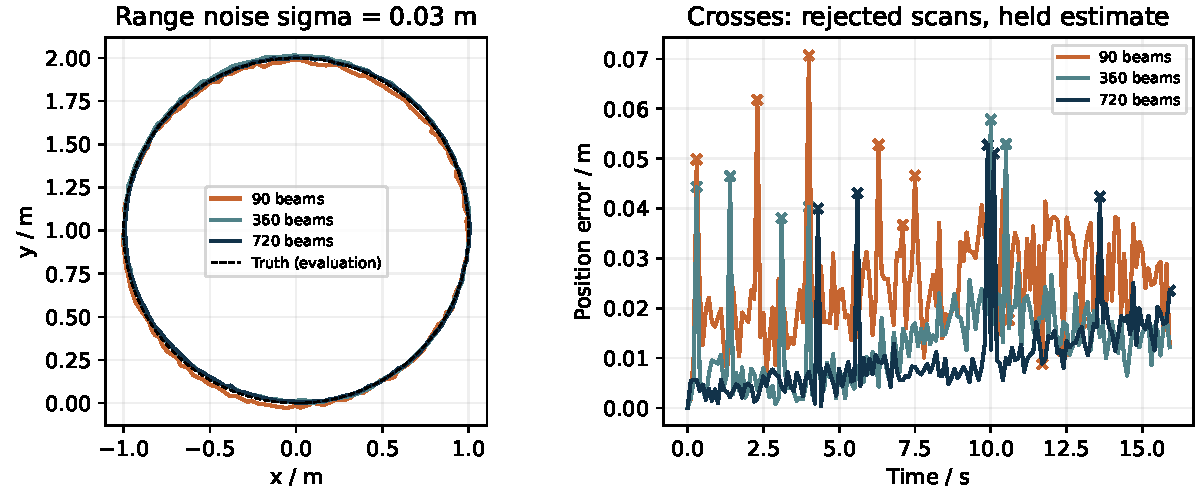
\includegraphics[width=\textwidth]{figures/ch08_odometry.pdf}
\caption{首帧对齐后的轨迹与位置误差。叉号是拒绝帧，此时画出保持上次估计的误差；圆轨迹保持等比例。}
\end{figure}

默认 ROS 实验的 0 到 3 s 共 31 次扫描中，30 次成功、1 次拒绝，
成功帧最大位置误差约 0.00214 m。这是一个固定种子小场景，不能推广为普遍精度承诺。
教材的六组回放也没有在配准后用真值修正结果。720 束不保证每项指标都优于 360 束：
法向量、关联和噪声共同影响局部优化。

\textbf{本章验收：}核心测试覆盖独立差分、恢复、退化、缺帧和有限窗口；
实际 ROS 核对输入隔离、采样时刻、点云/地图、暂停与重播。
继续实验时，一次只改一个参数，记录成功率、误差及失败状态。
下一章使用原始 IMU 预测和激光校正，在同一时间轴上估计速度与偏置。

\chapter{让 IMU 预测，让激光纠偏}
\begin{notebox}
\textbf{目标}\quad 在同一时间轴上估计位置、速度、航向与偏置，理解预测和校正的分工。\\
\textbf{先修}\quad 第 06、08 章；本章逐步解释协方差和卡尔曼增益。
\end{notebox}

\section{先单独验证滤波器}
重新构建并加载工作区后，从仓库根目录运行：
\begin{lstlisting}[language=bash,numbers=none]
ros2 run motion2d planar_ekf_demo tmp/ch09_filter
/usr/bin/python3 scripts/plot_ch09_filter.py
\end{lstlisting}
先把两个问题分开：滤波器的矩阵是否正确，真实扫描匹配能否提供可靠观测？
这个实验只检查前者。位姿输入是从解析轨迹生成的带噪合成测量，\emph{不是激光 SLAM 验证}。
后续在线版本才使用第八章扫描匹配的实际输出。

IMU 给短时间运动变化；它并不知道初始速度或全局位置。
位姿观测虽然较慢，却可以修正累积误差，并通过时间关联帮助估计速度与偏置。
二者噪声模型不同，不能简单把两个位置取平均。

\section{八个数描述平面状态}
采用状态列向量
\begin{equation}
x=(p_x,p_y,v_x,v_y,\psi,b_{ax},b_{ay},b_g)^\top.
\end{equation}
$p,v$ 在 odom 系，$\psi$ 是航向；加计偏置 $b_a$ 在机体系，单位 m/s$^2$；
陀螺偏置 $b_g$ 单位 rad/s。原始 IMU 的 orientation 字段不参与计算。
因为机器人水平运动且 roll、pitch 为零，重力没有 x/y 分量：
\begin{equation}
a_k=R(\psi_k)(f_{xy,k}-b_{a,k}),\quad
\omega_k=\omega_{m,k}-b_{g,k}.
\end{equation}
对时长 $h$ 的一个小区间，用步首航向旋转并保持加速度，得到
\begin{equation}
\begin{aligned}
p_{k+1}&=p_k+h v_k+\tfrac12 h^2a_k, &v_{k+1}&=v_k+h a_k,\\
\psi_{k+1}&=\operatorname{wrap}(\psi_k+h\omega_k), &b_{k+1}&=b_k.
\end{aligned}
\end{equation}
这是离散近似：连续转动时，区间内的 $R$ 实际也在变化。
缩短步长可以减小该近似误差；不能把公式说成一般旋转运动的精确积分。
当前内核接受 $0<h\leq0.1$ s，长时间缺测应报告失效而不是一步越过。

\clearpage
\section{不确定性如何沿着状态传播}
协方差 $P$ 的对角项描述方差，非对角项描述两个误差的关联。
例如位置与速度相关后，一个位置校正也能改变速度。
令 $J=\left[\begin{smallmatrix}0&-1\\1&0\end{smallmatrix}\right]$，
$A_\psi=R(\psi)J(f_{xy}-b_a)$。状态转移雅可比中的几个关键块为
\begin{equation}
\begin{aligned}
F_{pv}&=hI,&F_{p\psi}&=\tfrac12h^2 A_\psi,&F_{v\psi}&=h A_\psi,\\
F_{pb_a}&=-\tfrac12h^2R,&F_{vb_a}&=-hR,&F_{\psi b_g}&=-h.
\end{aligned}
\end{equation}
剩余对角块为单位阵。下列真实源码同时构造一步状态、$F$ 和噪声输入雅可比 $G$：
\lstinputlisting[language=C++,linerange={imu_predict_begin-imu_predict_end},
  includerangemarker=false]{../ros2_ws/src/motion2d/src/estimation/imu_predictor.cpp}

设本次采样的测量方差为
$\Sigma_u=\operatorname{diag}(\sigma_{ax}^2,\sigma_{ay}^2,\sigma_g^2)$，则
\begin{equation}
P^-_{k+1}=F_kP^+_kF_k^\top+G_k\Sigma_u G_k^\top+Q_b.
\end{equation}
第六章配置的是\textbf{每采样}标准差，所以例如速度方差增量为 $h^2\sigma_a^2$，
位置与速度的互协方差增量为 $\tfrac12 h^3\sigma_a^2$。
不能直接套用连续白噪声密度的 $h\sigma_a^2$ 公式。

偏置固定零时，最后三个状态及其协方差保持零。
开启 estimate\_bias 后，偏置初始标准差默认为 $(.05,.05,.01)$；
另设随机游走标准差 $\sigma_b=(.0005,.0005,.0001)$，它们是每 $\sqrt{\rm s}$ 的量。
因此 $Q_b$ 只在偏置对角块添加 $h\operatorname{diag}(\sigma_b^2)$。
这描述缓慢变化的不确定性，不等于模拟器一定注入了随机游走。

\clearpage
\section{一次位姿校正为什么也能改变速度}
观测向量 $z=(p_x^{\rm obs},p_y^{\rm obs},\psi^{\rm obs})$，$H$ 只选择状态中的位置和航向。
创新、创新协方差与增益为
\begin{equation}
r=z-Hx^-,\qquad S=HP^-H^\top+R_z,\qquad K=P^-H^\top S^{-1}.
\end{equation}
$r$ 的航向分量必须用 wrap 归一化。例如预测 $179^\circ$、观测 $-179^\circ$，
应校正约 $2^\circ$，而非 $-358^\circ$。\textbf{练习 ch09-1} 补完 yaw\_residual.hpp；
程序检查跨界、多圈及恰好 $\pi$ 的边界。

代码使用线性方程求解，不显式求逆。先检查 $r^\top S^{-1}r\leq16.3$，
不满足则拒绝本次校正。门限只能检查观测与当前模型是否相容，无法判定哪一方一定正确。
若模型漏掉了真实偏置，过小的 $P$ 反而会让它拒绝正常观测。

接受时 $x^+=x^-+Kr$。为减少数值误差对协方差的破坏，采用 Joseph 形式：
\begin{equation}
P^+=(I-KH)P^-(I-KH)^\top+K R_z K^\top.
\end{equation}
\lstinputlisting[language=C++,linerange={ekf_correct_begin-ekf_correct_end},
  includerangemarker=false]{../ros2_ws/src/motion2d/src/estimation/planar_ekf.cpp}

$K$ 的速度、偏置行通常并不为零，因为此前预测已经建立了互协方差。
这就是只有位置/航向观测仍能间接校正其他状态的原因。没有运动变化或长期缺少外部观测时，
这些量也可能很难区分；算法不能凭空产生可观测性。

\begin{notebox}
\textbf{教学模型的边界}\quad 激光局部地图和当前估计共享历史，观测不是严格独立的。
固定 $R_z$ 也只是可解释的测量尺度。这里的 EKF 不宣称严格统计一致，
更不能用很小的协方差数字证明定位准确。
\end{notebox}

\section{偏置与一秒缺测实验}
合成轨迹为 $p=(\sin(0.6t),\;0.5[1-\cos(0.6t)])$ m、$\psi=0.6t$ rad。
使用 200 Hz IMU、10 Hz 位姿观测、20 s 时长，4 到 5 s 不提供位姿校正。
同一组噪声输入同时送给三个滤波器；seed=9090。
加计偏置为 $(.08,-.04)$ m/s$^2$，陀螺偏置为 $.01$ rad/s，滤波器没有收到这些答案。
初始速度先验为零、标准差 1 m/s；实际初速不为零，因此纯 IMU 还包含初速不可知的误差。

\clearpage
\begin{figure}[t]
\centering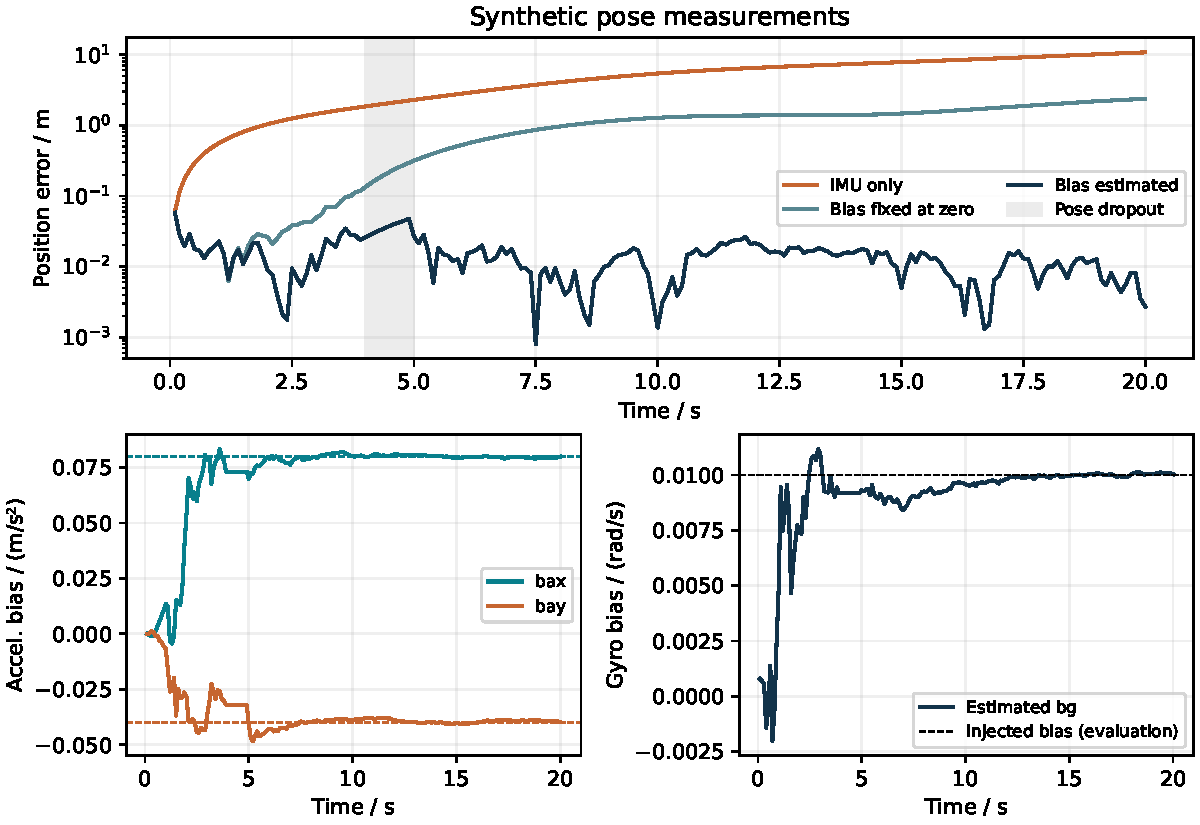
\includegraphics[width=\linewidth]{figures/ch09_filter.pdf}
\caption{合成位姿传感器实验。上图纵轴为对数，灰带表示停止位姿校正；下图虚线只用于评估注入的偏置。}
\end{figure}
\begin{center}\small
\pgfplotstabletypeset[col sep=comma,string type,
columns={mode,rmse,dropout_rmse,accepted,rejected},
columns/mode/.style={column name=模式,string replace*={imu_only}{仅 IMU},
  string replace*={fixed_zero_bias}{偏置固定零},string replace*={estimate_bias}{估计偏置}},
columns/rmse/.style={column name=全程 RMSE/m,fixed,precision=4,string type=false},
columns/dropout_rmse/.style={column name=缺测段 RMSE/m,fixed,precision=4,string type=false},
columns/accepted/.style={column name=接受},columns/rejected/.style={column name=拒绝},
every head row/.style={before row=\toprule,after row=\midrule},
every last row/.style={after row=\bottomrule}]{data/ch09_filter.csv}
\end{center}
表中误差统计全部 4000 个 IMU 时刻，接受/拒绝计数只针对低频位姿校正。
偏置固定零时，模型误差积累并触发大量拒绝；启用偏置估计后，本例全程位置 RMSE 约 0.0184 m。
这说明模型与置信度需要匹配，不意味着启用偏置状态在所有场景都更好。

\textbf{练习与验收：}手推 $F_{v\psi}$；完成角度残差练习；把注入偏置改为零后复跑，
再把观测标准差减半，比较误差及拒绝数。测试还核对常加速度解析解、$F/G$ 中心差分、
互协方差、离群点拒绝以及长时间更新后的协方差对称性与半正定性。
在线时间对齐将在下一个功能接入，不用合成观测实验冒充真实雷达定位。

\chapter{回到起点之后：关键帧与位姿图}
\begin{notebox}
\textbf{目标}\quad 用相对运动约束共同调整轨迹，并按新位姿重建观测地图。\\
\textbf{先修}\quad 第 02、08、09 章的坐标变换、最小二乘和传感器融合。
\end{notebox}

\section{从一条链变成一张图}
机器人逐帧估计运动，微小误差会随路程积累。走一圈回到熟悉的墙角时，
里程计的终点可能偏离起点。此时旧扫描和新扫描提供了额外信息：
这两个时刻其实看到了同一个地点，它们的相对位置可以再测一次。
这条跨越很长时间的约束称为\textbf{回环边}。

先运行一个可以直接指定相对位姿的实验：
\begin{lstlisting}[language=bash]
ros2 run motion2d pose_graph_demo tmp/ch10_graph
/usr/bin/python3 scripts/plot_ch10_graph.py
\end{lstlisting}
81 个节点沿 $4\times3$ m 矩形行走，每条相邻节点之间的测量都带有小误差。
把这些测量依次复合，得到逐渐漂移的链。最后加入“末帧与首帧重合”的测量，
优化器就会让所有节点共同调整。本章先弄清这个调整过程，再从实际扫描中寻找回环。

\subsection{先手算只有三个位置的图}
为了看清“共同调整”，暂时只考虑一维。固定 $x_0=0$，
顺序测量是 $x_1-x_0\approx1$ m、$x_2-x_1\approx1$ m，
额外测量却说 $x_2-x_0\approx1.8$ m。
三条边不能同时精确满足；令每条边采用相同的尺度，最小化残差平方和：
\begin{equation}
C(x_1,x_2)=\tfrac12[(x_1-1)^2+(x_2-x_1-1)^2+(x_2-1.8)^2].
\end{equation}
分别求偏导，注意第二项中 $x_1$ 的系数为 $-1$：
\begin{align}
\frac{\partial C}{\partial x_1}&=(x_1-1)-(x_2-x_1-1)=2x_1-x_2=0,\\
\frac{\partial C}{\partial x_2}&=(x_2-x_1-1)+(x_2-1.8)=-x_1+2x_2-2.8=0.
\end{align}
第一式给出 $x_2=2x_1$，代入第二式得到 $x_1=.9333$ m、$x_2=1.8667$ m。
三个残差分别约为 $-.0667,-.0667,+.0667$ m：新增测量与原来的两个测量各分担了一部分误差。

\begin{center}
\begin{tikzpicture}[x=1cm,y=1cm,>=Stealth,
  pose/.style={circle,draw=navy,fill=pale,minimum size=8mm}]
\node[pose,rectangle] (a) at (0,0) {$x_0$};
\node[pose] (b) at (4,0) {$x_1$};
\node[pose] (c) at (8,0) {$x_2$};
\draw[->,thick] (a)--node[above]{测得 $1$ m}(b);
\draw[->,thick] (b)--node[above]{测得 $1$ m}(c);
\draw[->,tealblue,thick] (a.south) to[out=-55,in=-125] node[below]{额外测得 $1.8$ m} (c.south);
\node[above=7mm] at (a) {固定 $0$};
\node[above=7mm] at (b) {$1\ \to\ .9333$};
\node[above=7mm] at (c) {$2\ \to\ 1.8667$};
\end{tikzpicture}
\end{center}
图中的位置变量可以换成二维位姿，边也可以带不同的可信程度。
接下来的计算就是把这个小例子推广到位置与航向一起变化的情况。

\section{二维边残差：比较预测与测量}
每个节点保存关键帧在 map 中的位姿 $T_i=(R_i,p_i)$，
它把帧 $i$ 中的点变到 map。边测量 $Z_{ij}=(R_z,z_{ij})$ 把帧 $j$ 的点变到帧 $i$。
由第二章的逆变换与复合规则，当前节点预测的相对变换为
\begin{equation}
T_i^{-1}T_j=(R_i^\top R_j,\ q),\qquad q=R_i^\top(p_j-p_i).
\end{equation}
$q$ 是“站在第 $i$ 帧看，第 $j$ 帧原点在哪里”。
若预测与测量一致，$Z_{ij}^{-1}T_i^{-1}T_j$ 就等于单位变换。
再做一次复合，得到误差变换的平移与角度：
\begin{equation}
e_{ij}=\begin{bmatrix}R_z^\top(q-z_{ij})\\
\operatorname{wrap}(\psi_j-\psi_i-\psi_{ij})\end{bmatrix}.
\end{equation}
前两项先在 $i$ 帧中相减，再旋转到测量所定义的 $j$ 帧方向；最后一项比较相对航向。
本章直接用这三个数度量误差，所需运算都是二维旋转、平移和角度归一化。

例如 $p_i=(1,2)$ m、$\psi_i=90^\circ$，$p_j=(1,4)$ m、$\psi_j=90^\circ$，
则 $q=R(-90^\circ)(0,2)=(2,0)$ m，相对航向为零。
当测量也为 $z_{ij}=(2,0)$ m、$\psi_{ij}=0$ 时，残差为零。
如果只把 $p_j$ 的全局 $x$ 增加 $.1$ m，$q$ 变成 $(2,-.1)$ m，残差为 $(0,-.1,0)$。
全局向右的小误差，在朝向北的 $i$ 帧中表现为向右侧，即局部 $y$ 负方向。

\subsection{把米和弧度换成统一的误差尺度}
给残差三个方向指定标准差 $\sigma_x,\sigma_y,\sigma_\psi$，分别除以标准差：
\begin{equation}
D_{ij}=\operatorname{diag}(1/\sigma_x,1/\sigma_y,1/\sigma_\psi),\qquad
\widetilde e_{ij}=D_{ij}e_{ij}.
\end{equation}
每个新分量表示偏离了多少个标准差，已经没有单位。这个操作称为白化，
这里采用三个方向相互独立的测量尺度；它们对应上式残差所在的坐标方向。
例如残差 $(.06,0,.04)$、尺度 $(.03,.03,.02)$，得到 $(2,0,2)$，
平方代价为 $\tfrac12(2^2+0^2+2^2)=4$。
尺度减半时，相同误差的平方代价变为四倍，所以该约束会更强地影响轨迹。

顺序边使用 $\tfrac12\|\widetilde e\|^2$；回环边对范数使用第八章的 Huber 损失，
默认阈值为 3。它让很大的回环残差以线性速度增加代价，降低单条异常边对整张图的拉动。

\section{固定第一帧，就是给地图选坐标原点}
只有相对测量时，把整张图平移或转动都不会改变测量预测。
设所有位姿同时左乘固定变换 $A$，利用 $(AT_i)^{-1}=T_i^{-1}A^{-1}$，有
\begin{equation}
(AT_i)^{-1}(AT_j)=T_i^{-1}A^{-1}AT_j=T_i^{-1}T_j.
\end{equation}
也就是说，同一组相对残差对应无数张整体位置和朝向不同的图。
在最小二乘方程里，这表现为有些增量方向不会改变代价，因而解不唯一。
一维小例子若连 $x_0$ 也一起优化，给三个 $x$ 同时加任意常数就会发生这种情况。

固定首帧的 $x,y,\psi$ 后，地图的三个整体自由度就确定了。
代码把节点 0 留在原处，只把节点 $1,\ldots,N-1$ 的三个数写进优化变量，
总维数为 $3(N-1)$。首帧数值来自坐标原点的选择，可以取零，也可以取其他给定位置。
若图包含互不连接的两部分，第二部分仍可自行平移旋转，
因此程序用图遍历检查所有节点能否从首帧到达，并以 \code{disconnected} 提示缺少连接约束。

\section{对一条边的两端分别求导}
采用加法更新 $p_i\leftarrow p_i+\delta p_i$、$\psi_i\leftarrow\psi_i+\delta\psi_i$。
记 $J=\left[\begin{smallmatrix}0&-1\\1&0\end{smallmatrix}\right]$。
由 $q=R_i^\top(p_j-p_i)$ 直接得到
\begin{equation}
\frac{\partial q}{\partial p_i}=-R_i^\top,\quad
\frac{\partial q}{\partial p_j}=R_i^\top,\quad
\frac{\partial q}{\partial\psi_i}=-Jq,\quad
\frac{\partial q}{\partial\psi_j}=0.
\end{equation}
第三项可从 $R_i^\top=R(-\psi_i)$ 看出：对 $\psi_i$ 求导为 $-JR_i^\top$，再乘位置差。
第四项为零，是因为改变末帧的朝向并不改变它的原点位置。
测量 $R_z,z_{ij}$ 在求导时保持不变，因此 $e_p=R_z^\top(q-z_{ij})$ 的每一块偏导
只需在左边再乘 $R_z^\top$。角度残差对两端航向的导数分别为 $-1,+1$，于是
\begin{align}
A_{ij}=\frac{\partial e}{\partial(p_i,\psi_i)}
&=\begin{bmatrix}-R_z^\top R_i^\top&-R_z^\top Jq\\0\;0&-1\end{bmatrix},\\
B_{ij}=\frac{\partial e}{\partial(p_j,\psi_j)}
&=\begin{bmatrix}R_z^\top R_i^\top&0\\0\;0&1\end{bmatrix}.
\end{align}
例如 $R_i=R_z=I$、$q=(2,1)$ m，则
\begin{equation}
A=\begin{bmatrix}-1&0&1\\0&-1&-2\\0&0&-1\end{bmatrix},\qquad B=I.
\end{equation}
只增加起点航向 $.01$ rad，预测残差约变化 $(.01,-.02,-.01)$。
可以用这个数值例子核对源码的 \code{q.y(), -q.x()} 符号。
航向残差跨越 $\pm\pi$ 时先归一化；中心差分的两次扰动应落在同一角度分支内，检验局部导数。

\par\noindent\begin{minipage}{\linewidth}
\lstinputlisting[language=C++,linerange={graph_residual_begin-graph_residual_end},
  includerangemarker=false]{../ros2_ws/src/motion2d/src/estimation/pose_graph.cpp}
\end{minipage}\par

\section{把许多小方程装成一个大方程}
一条边只依赖两端节点。将白化雅可比记为 $J_i=DA$、$J_j=DB$，
一阶近似为 $\widetilde e(\delta)\approx\widetilde e+J_i\delta_i+J_j\delta_j$。
第八章已从残差平方和推得 $H\delta=-g$。现在对这一条边展开二次代价，
与两端有关的贡献恰好是
\begin{equation}
\begin{bmatrix}H_{ii}&H_{ij}\\H_{ji}&H_{jj}\end{bmatrix}
\mathrel{+}=w\begin{bmatrix}J_i^\top J_i&J_i^\top J_j\\
J_j^\top J_i&J_j^\top J_j\end{bmatrix},\qquad
\begin{bmatrix}g_i\\g_j\end{bmatrix}\mathrel{+}=w\begin{bmatrix}J_i^\top\widetilde e\\J_j^\top\widetilde e\end{bmatrix}.
\end{equation}
$\mathrel{+}=$ 表示把本条边的贡献加到已有数值上。
普通边 $w=1$；由第八章的 Huber 导数得到回环权重
$w=\min(1,3/\|\widetilde e\|)$，零残差时取 1。
每个 $H_{ij}$ 都是 $3\times3$ 小块，没有边相连的节点对不会直接贡献块。
因此尽管图有很多节点，矩阵中仍有大量零，称为\textbf{稀疏矩阵}。

节点 $k\geq1$ 对应大向量从 $3(k-1)$ 开始的三个位置。
下面代码对一条边的两个端点分别遍历，跳过固定节点，把四个小块按行列位置装进去。
\code{Triplet} 存储“行、列、值”；\code{setFromTriplets} 会把落在同一位置的值相加。

\par\noindent\begin{minipage}{\linewidth}
\lstinputlisting[language=C++,linerange={graph_assembly_begin-graph_assembly_end},
  includerangemarker=false]{../ros2_ws/src/motion2d/src/estimation/pose_graph.cpp}
\end{minipage}\par

在三个位置的一维例子中，收集各边偏导可得
$H=\left[\begin{smallmatrix}2&-1\\-1&2\end{smallmatrix}\right]$。
在初值 $(x_1,x_2)=(1,2)$ 处，$g=(0,.2)^\top$。
解 $H\delta=-g$ 得 $\delta=(-.0667,-.1333)^\top$，正好得到本章开头的答案。
二维问题的旋转是非线性的，所以更新后要重新计算残差和雅可比，再求下一步。

\subsection{为什么有时只走半步}
一阶近似在增量较小时更可靠。求出 $\delta$ 后，先尝试完整增量，
若实际代价下降不够，再尝试 $\delta/2,\delta/4,\ldots$，称为回溯线搜索。
设当前总代价为 $C$，沿增量方向的一阶变化率是 $g^\top\delta$。
因为 $H\delta=-g$，正定时
$g^\top\delta=-\delta^\top H\delta<0$，这是一个下降方向。
代码用条件
\begin{equation}
C(x+\alpha\delta)\leq C(x)+10^{-4}\alpha g^\top\delta
\end{equation}
要求实际下降达到一阶预测下降量的一小部分，并依次尝试 $\alpha=1,1/2,\ldots,1/1024$。
所有增量分量都很小时报告收敛；若方程奇异、迭代耗尽或所有步长都被拒绝，
保留当前图并返回对应状态，便于检查初值和边约束。

\subsection{错误回环为何仍需先做几何检查}
考虑一个位置 $x$，正常测量为 1 m，错误回环测量为 10 m，两者标准差均为 $.1$ m。
普通平方代价的导数是 $100(x-1)+100(x-10)$，令其为零得到 $x=5.5$ m。
若只对回环用阈值 3 的 Huber，在 $x$ 接近 1 时，回环白化残差为 $10(x-10)<-3$，
Huber 对它的导数为 $-3$，再乘链式因子 10，得到对 $x$ 的导数 $-30$。
总导数于是变成 $100(x-1)-30$，最优位置为 $x=1.3$ m，且满足所用的线性分支条件。
鲁棒损失把错误回环的拉力限制住了，仍然留下 $.3$ m 偏移。
所以回环进入图之前，还需要检查两帧点云是否重叠、配准是否稳定和往返变换是否一致。

\clearpage
\section{矩形实验与可独立检验的答案}
固定 seed=1010，沿四条边各走 20 步。每步加独立 $0.01$ m 平移噪声、$0.002$ rad 航向噪声，
并注入每步 $0.003$ rad 航向偏差。顺序边的测量尺度为 $(.03,.03,.02)$；
闭环观测为单位变换，尺度 $(.02,.02,.01)$。参考轨迹仅用于评估，不送给优化器。
\begin{figure}[h]
\centering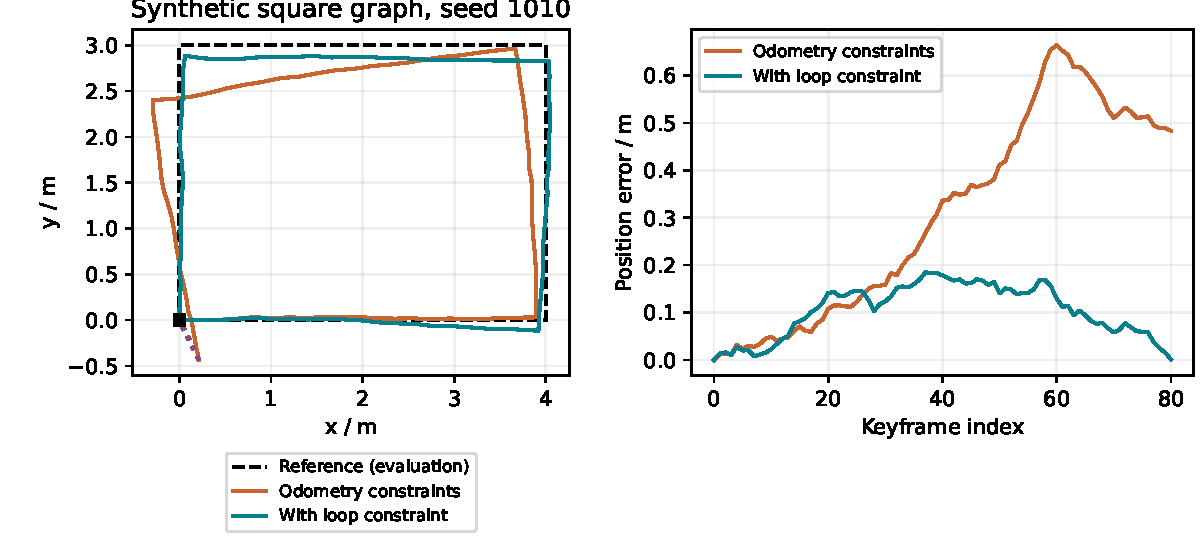
\includegraphics[width=\linewidth]{figures/ch10_graph.pdf}
\caption{合成位姿图的优化前后结果。左图等比例，方块为固定首帧，紫色虚线指出原始链的闭合缺口。}
\end{figure}
\begin{center}\small
\pgfplotstabletypeset[col sep=comma,
columns={mode,position_rmse,closure_error,final_cost,iterations},
columns/mode/.style={column name=约束,string type,string replace*={odometry}{顺序边},string replace*={loop}{加回环}},
columns/position_rmse/.style={column name=位置 RMSE/m,fixed,precision=4},
columns/closure_error/.style={column name=闭合误差/m,fixed,precision=4},
columns/final_cost/.style={column name=最终代价,fixed,precision=4},
columns/iterations/.style={column name=迭代},
every head row/.style={before row=\toprule,after row=\midrule},
every last row/.style={after row=\bottomrule}]{data/ch10_graph.csv}
\end{center}
顺序边代价几乎为零，因为链本身就是由这些边累乘出来的：每个相邻位姿都精确满足带误差的测量。
加入新约束后边之间有冲突，最优代价可以大于零，而参考误差反而下降。
因此，代价衡量图内约束的吻合程度，位置 RMSE 则衡量相对于参考轨迹的误差；应结合两者解释结果。

\textbf{练习 ch10-1：}补完 edge\_residual.hpp，检查旋转坐标和角度跨界。
理解题证明左乘不变性；实验题改变回环尺度，比较全程 RMSE、闭合误差、代价与求解状态。
常见错误包括变换乘法顺序颠倒、只锚定位置却漏掉航向、把错误闭环交给鲁棒核“自动判断”。

\textbf{手算练习：}在三节点例子中将额外边的标准差减半。
这相当于把它的平方项乘以 4；重新求两个偏导为零的方程，观察误差如何重新分配。

\clearpage
\section{从关键帧中寻找旧地点}
完整管线沿用第九章前端；后端只接收扫描及同一采样时刻的校正位姿。
平移达到 0.3 m、航向变化达到 0.25 rad，或距上帧达到 2 s，就保存一个关键帧。
其中既有原始距离数组，也有机体系的体素点云和局部法向量。
机体系观测保留了采样时的原始几何，后面改变关键帧的全局位姿时，可用它重新投影地图。

\begin{lstlisting}[language=bash]
ros2 launch motion2d_bringup ch10.launch.py rviz:=false
# Another terminal, same ROS environment, repository root:
/usr/bin/python3 scripts/check_ch10.py
\end{lstlisting}
排除最近 20 个关键帧后，只在当前估计位置的 0.8 m 范围内寻找候选，航向差小于 0.6 rad。
每次最多检查距离最近的三个候选。候选搜索以当前估计为中心，适合累计漂移仍小于搜索半径的场景。漂移超过半径时，旧地点会落在窗口之外；扩大窗口能找回更多候选，也会增加误匹配的机会。
成功回环后至少等待五个新关键帧，避免高频重复加入同一个地点的相关证据。

\begin{center}\small
\begin{tabular}{ll}\toprule
几何检查 & 默认条件 \\\midrule
双向点到线 ICP & 两个方向都收敛，且没有秩退化 \\
有效对应比例 & 两个方向均至少 $55\%$ \\
残差与初值偏离 & RMSE 不超过 0.05 m；校正不超过 0.5 m / 0.25 rad \\
往返一致性 & 平移不超过 0.03 m，航向不超过 0.02 rad \\\bottomrule
\end{tabular}
\end{center}
若正向变换为 $T_{ij}$，反向为 $T_{ji}$，则一致时 $T_{ij}T_{ji}\approx I$。
将正向变换写成 $(R_f,t_f)$、反向变换写成 $(R_b,t_b)$，复合后的平移为
$t_f+R_ft_b$，角度为 $\operatorname{wrap}(\psi_f+\psi_b)$。
例如正向平移 $(1,0)$ m、转 $90^\circ$，反向应平移 $(0,1)$ m、转 $-90^\circ$；
因为 $R(90^\circ)(0,1)=(-1,0)$，往返平移才会相消。
下面代码按这个复合公式检查；通过各项门限后才生成回环边。
\lstinputlisting[language=C++,linerange={loop_cycle_begin-loop_cycle_end},
  includerangemarker=false]{../ros2_ws/src/motion2d/src/estimation/loop_closure.cpp}

平行长墙沿墙方向缺少约束，可由第八章的秩检查识别。
重复房间则可能在两个方向都得到相似的点云：即使往返变换很小，仍需结合更长时间的运动历史
或更有辨识度的场景特征区分地点。可以主动构造这两种场景，分别观察退化拒绝和地点混淆。
图优化失败时撤掉新回环边，继续使用已有的局部里程计和顺序边。

当前最多保留 200 个关键帧，达到容量后以 \code{capacity_reached} 提示停止加入新帧。
关键帧越多，逐帧重建地图的计算量也越大；更大场景可将若干关键帧组成子图，按子图组织更新。

\clearpage
\section{回环更新地图坐标，不改写局部里程计}
同一机器人有局部位姿 $T_{OB}$ 和图优化后的全局位姿 $T_{MB}$，满足
\begin{equation}
T_{MB}=T_{MO}T_{OB},\qquad T_{MO}=T_{MB}T_{OB}^{-1}.
\end{equation}
第二式由第一式在右边乘 $T_{OB}^{-1}$ 得到。展开为旋转和平移，就是
\begin{equation}
R_{MO}=R_{MB}R_{OB}^\top,\qquad
p_{MO}=p_{MB}-R_{MO}p_{OB}.
\end{equation}
例如同一关键帧的全局位姿为 $p_{MB}=(10,-2)$ m、$\psi_{MB}=180^\circ$，
局部位姿为 $p_{OB}=(2,1)$ m、$\psi_{OB}=90^\circ$。
则校正旋转为 $90^\circ$，先算 $R_{MO}p_{OB}=(-1,2)$，再相减得到 $p_{MO}=(11,-4)$ m。
将其代回 $p_{MB}=p_{MO}+R_{MO}p_{OB}$，即可核对 $(10,-2)$。
程序用最新关键帧的两种位姿计算这个校正，原始 odom 位姿继续保存自己的运动历史。
\textbf{练习 ch10-2} 完成 map\_alignment.hpp，先手算带 $90^\circ$ 旋转的例子。
仅把两个位置相减会漏掉旋转，无法得到正确变换。

\lstinputlisting[language=C++,linerange={map_alignment_begin-map_alignment_end},
  includerangemarker=false]{../ros2_ws/src/motion2d/src/estimation/keyframes.cpp}

一条 TF 边只有一个发布者：SLAM 发布 map 到 odom；estimated 适配器发布 odom 到 base\_link；
模拟器只保留圆心处传感器的静态外参。回环可以让机器人在 map 中跳到更一致的位置，
但不会把这个全局位移直接写入局部运动链。第十九章会处理全局目标与局部控制参考的衔接。

\begin{center}\small
\begin{tabular}{ll}\toprule
输出 & 含义 \\\midrule
\texttt{/map/cloud} 与 \texttt{/map} & 按最新图位姿重建的点云与观测栅格 \\
\texttt{/path/graph\_before} & 固定首帧基准中的原始里程计关键帧 \\
\texttt{/path/graph\_after} & 同一基准中的优化关键帧 \\
\texttt{/slam/edges} & 顺序边与紫色回环边 \\
\texttt{/slam/status} & 更新/拒绝状态及关键帧、回环计数 \\\bottomrule
\end{tabular}
\end{center}
前后路径都用首帧固定的 map 基准比较，不再用当前 map 到 odom 把原始基线变换第二次。
高频局部轨迹仍由第九章输出；图更新频率是关键帧频率。

\textbf{为什么要重建：}设旧图在 $x=3$ m 有一面墙，优化后这次观测应落在 $x=4$ m。
直接追加新点会留下两面墙。重建时新建空栅格，再遍历所有保留的原始扫描，
按照各自优化后的采样位姿重新做射线清空与端点占据；体素点云也重新生成。
本章累积的是关键帧的实际观测，未被光线照到的区域保留未知状态。

只改一条全局 TF，也无法修正不同历史帧之间的相对错位。
设旧点云中两个点为 $u,v$，施加相同刚体变换后，它们的距离仍为
\begin{equation}
\|(Ru+t)-(Rv+t)\|=\|R(u-v)\|=\|u-v\|.
\end{equation}
最后一步使用 $R^\top R=I$：旋转保持长度。
因此要把两次错开的墙面观测重新对齐，就必须分别使用各自优化后的关键帧位姿。

\begin{center}
\begin{tikzpicture}[x=1cm,y=1cm,>=Stealth,
  box/.style={draw=tealblue,fill=pale,rounded corners=2pt,align=center,minimum height=9mm}]
\node[box] (local) at (0,0) {各帧局部扫描};
\node[box] (pose) at (0,-1.6) {各帧优化位姿};
\node[box] (project) at (4,-.8) {逐帧重新投影};
\node[box] (map) at (8,-.8) {新栅格与点云};
\draw[->] (local.east)--(project.north west);
\draw[->] (pose.east)--(project.south west);
\draw[->] (project)--node[above=6mm,font=\small]{重新累积}(map);
\end{tikzpicture}
\end{center}

\clearpage
\section{实际激光与 IMU 的矩形回放}
\begin{lstlisting}[language=bash]
ros2 run motion2d slam_demo tmp/ch10_slam
/usr/bin/python3 scripts/plot_ch10_slam.py
\end{lstlisting}
使用 $14\times12$ m 房间，内部有一个圆与一个三角形。
半径 0.2 m 的全向圆盘沿 $6\times4$ m 矩形行走，每边 6 s，平滑的时间规律让它在拐角静止（第十四章推导这条五次曲线）；
机体 yaw 保持零。四条边均通过整段扫掠检查。
360 束、距离噪声 0.03 m、激光 10 Hz、IMU 200 Hz，噪声 seed=4242/6060。

\begin{figure}[h]
\centering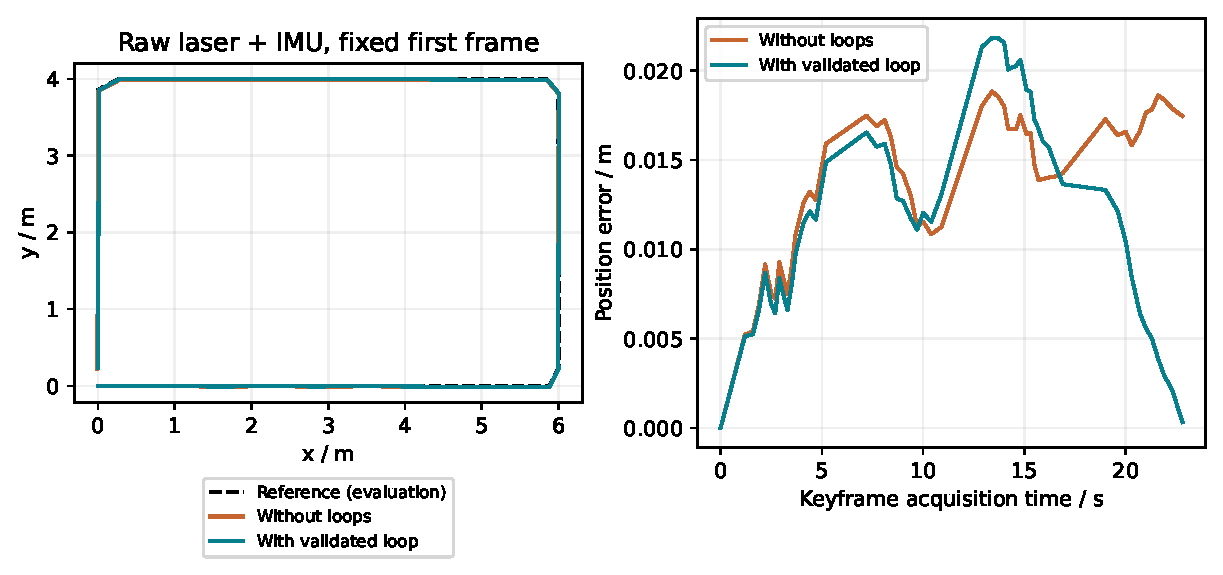
\includegraphics[width=\linewidth]{figures/ch10_slam.pdf}
\caption{同一真实传感器前端输出，分别送给回环关闭和开启的图。误差只统计关键帧；参考轨迹仅用于评估。}
\end{figure}
\begin{center}\small
\pgfplotstabletypeset[col sep=comma,
columns={mode,keyframes,loops,position_rmse,final_position_error},
columns/mode/.style={column name=模式,string type,string replace*={no_loop}{关闭回环},string replace*={loop}{开启回环}},
columns/keyframes/.style={column name=关键帧},columns/loops/.style={column name=回环},
columns/position_rmse/.style={column name=位置 RMSE/m,fixed,precision=4},
columns/final_position_error/.style={column name=末关键帧误差/m,fixed,precision=4},
every head row/.style={before row=\toprule,after row=\midrule},
every last row/.style={after row=\bottomrule}]{data/ch10_slam.csv}
\end{center}
本例在 22.3 s 检查一个候选并接受回环；最后关键帧时间为 22.8 s。
表中的末帧误差取 22.8 s 的关键帧位置与同一时刻参考位置之差；首尾闭合距离则取末帧与首帧之差，两者使用的参照不同。
激光拒绝 27 帧，EKF 无额外拒绝；失败扫描没有进入图。

回环显著改善了靠近返回地点的关键帧，但部分中间点误差反而略增。
全程位置 RMSE 从约 1.44 cm 降至 1.32 cm；末帧误差则从约 1.75 cm 降至 0.033 cm。末帧接近回环约束的位置，因而改善更明显；其他节点还要兼顾沿途顺序边。
所有 CSV、原始地图 PGM 与点云 CSV 均可由上述命令重新生成。

\clearpage
\section{从地图中观察回环的作用}
\begin{figure}[h]
\centering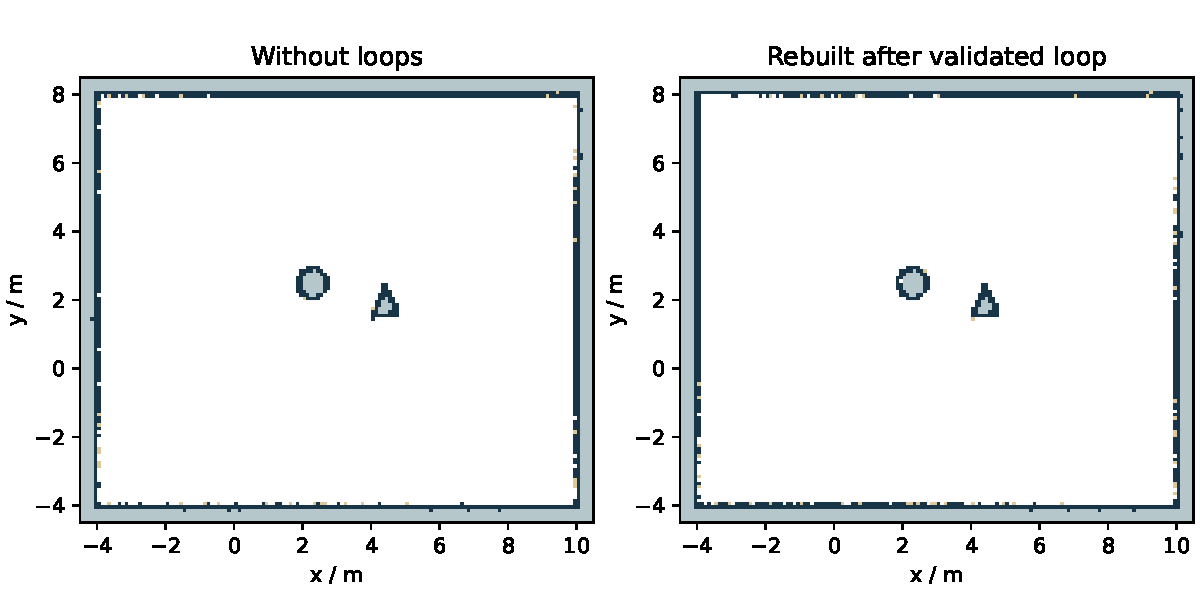
\includegraphics[width=\linewidth]{figures/ch10_maps.pdf}
\caption{两图均由关键帧扫描构建，分辨率 0.1 m。白色自由，深色占据，灰色未知，浅褐色为已观测但不确定；横纵尺度相同。}
\end{figure}
本例原始误差只有厘米量级，小于地图分辨率，因此两张全景图很接近。
可以做一个更容易看清的实验：只把某个关键帧的墙面观测位姿移动一个格子，分别尝试追加与重建。
追加会留下旧墙，重建则根据所有关键帧的新位姿重新决定每个格子的证据。
圆与三角形内部没有被光线穿透，仍然保留未知区域。

启动默认 RViz 配置时，应看到优化关键帧、紫色回环边、重建点云和占据图；
原始世界与真值机器人默认隐藏。可修改配置中的 slam.enable\_loops 为 false 对照。
\begin{enumerate}
\item \textbf{理解：}为什么只有修改 TF、不重建历史点云，会得到坐标正确但几何仍旧扭曲的地图？
\item \textbf{代码：}完成两道练习，检查边残差的变换顺序和 map 到 odom 的计算。
\item \textbf{实验：}改变候选距离、关键帧间隔或激光噪声，记录候选数、接受数、拒绝帧与误差。
\item \textbf{失败：}用单面墙验证退化，用无重叠云验证拒绝；达到图容量时应看到明确状态。
\end{enumerate}

本章将激光/IMU 局部定位、几何回环和地图重建连成了一个小场景 SLAM 系统。
继续扩大场景时，可以研究全局地点识别、动态物体处理及子图管理。
下一章从真值定位和观测地图开始学习路径搜索，再逐步将规划与本章的定位建图结果连接起来。

\chapter{给圆盘找一条路：配置空间与 A*}
\begin{notebox}
\textbf{目标}\quad 将圆盘规划化成中心点搜索，理解栅格、未知区域、路径与轨迹的区别。\\
\textbf{先修}\quad 第 03、07 章。先在给定栅格上检查算法，再接观测地图。
\end{notebox}

\section{先运行一张带窄门的地图}
\begin{lstlisting}[language=bash]
ros2 run motion2d astar_demo tmp/ch11_astar
/usr/bin/python3 scripts/plot_ch11_astar.py
\end{lstlisting}
这次输入是手工给定的 $41\times31$ 栅格，分辨率 0.1 m。
中间隔墙有宽 0.7 m 的门；起点 $(.75,.75)$ m，终点 $(3.25,2.25)$ m。
改变半径，观察门从可通行变成不可达。该小实验隔离规划算法，不冒充未知环境建图。

\section{圆盘变成一个中心点}
设原始阻塞区域为 $\mathcal O$，圆盘物理半径为 $r$，额外安全裕量为 $m$。
中心点必须避开膨胀集合
\begin{equation}
\mathcal O_{\rm conf}=\mathcal O\oplus B(0,r+m).
\end{equation}
这里 $\oplus$ 表示将集合中的每个点向外扩张一个半径 $r+m$ 的圆。
半径与裕量只加一次；后面使用已经膨胀的地图时不能再重复扣除机器人半径。

原始占据栅格表示方格的\textbf{面积}，不是只有格子中心的一个点。
本章还要求输出自由格的整个闭区域都安全，方便后续构造走廊。
两个边长 $\rho$ 的格子，相对索引差为 $(\Delta i,\Delta j)$，其最小距离为
\begin{equation}
d_x=\rho\max(0,|\Delta i|-1),\qquad
 d_y=\rho\max(0,|\Delta j|-1),\qquad d=\sqrt{d_x^2+d_y^2}.
\end{equation}
若 $d\leq r+m$，候选格子被阻塞。相邻方格共享边或角时距离为零；接触也视为碰撞。
\lstinputlisting[language=C++,linerange={inflation_stencil_begin-inflation_stencil_end},
  includerangemarker=false]{../ros2_ws/src/motion2d/src/planning/inflation.cpp}

这种整格安全证书比只检查中心更保守。即使 $r=0$，与障碍接触的相邻格仍会被排除。
连续几何可以通过的窄门，粗网格可能判不可达；缩小 $\rho$ 能减少这类保守损失。
地图外部也视为阻塞，边界附近格子同样要满足距离要求。

\section{A* 的三个数与两种邻接}
$g(n)$ 是从起点到节点 $n$ 已知的最小代价，$h(n)$ 是到目标的下界，优先展开
\begin{equation} f(n)=g(n)+h(n). \end{equation}
四邻接每步长 $\rho$，使用 Manhattan 距离；八邻接另有长 $\sqrt2\rho$ 的对角步，使用 octile 距离。
设到目标的索引差绝对值为 $d_x,d_y$，则
\begin{align}
h_4 &= \rho(d_x+d_y),\\
h_8 &= \rho\bigl[\max(d_x,d_y)+(\sqrt2-1)\min(d_x,d_y)\bigr].
\end{align}
无障碍时这就是最短距离；障碍只会让路更长，因此不会高估。
它们还满足一致性，节点确定后不必反复重新打开。

\lstinputlisting[language=C++,linerange={astar_neighbors_begin-astar_neighbors_end},
  includerangemarker=false]{../ros2_ws/src/motion2d/src/planning/astar.cpp}

关键是中间的对角检查：终点自由不代表连线安全。
例如右邻格被堵、上邻格自由，即使右上格自由，也不能沿对角线擦过右邻障碍的角。
\textbf{练习 ch11-1} 补完 diagonal\_step.hpp，分别检查两侧被挡的情况。

程序保留每个节点的父节点，从目标反向回溯，再反转得到格子序列。
输出折线包含精确请求的起终点；它们可以不在格子中心。
因为起终格的整个面积已保证安全，格内接到中心的短线仍然安全。
两个点在同一格时直接相连，不必绕到格子中心。

\clearpage
\section{未知不是免费的捷径}
只有已观测且概率编码不大于 35 的格子作为原始自由格；未知 $-1$、不确定与占据均默认阻塞。
这是本课程的规划策略，不是 ROS 强制规定。显式设置 unknown\_blocked=false 可以做乐观探索实验，
但不能把未观测空间称为已验证安全。

搜索结果必须区分：
\begin{center}\small
\begin{tabular}{ll}\toprule
状态 & 含义 \\\midrule
found & 在当前栅格和规则下找到路径 \\
invalid\_start / invalid\_goal & 起点或终点越界、被堵或接触阻塞边界 \\
unreachable & 两点有效，但自由格图不连通 \\\bottomrule
\end{tabular}
\end{center}
失败时返回空路径和无穷大代价。成功的 grid\_cost 是\textbf{中心节点图}上的最短距离，
不是含精确端点及后续简化的折线总长。两者的定义不能混用。

\section{删掉折点之前，检查整条线段}
贪心简化从当前点开始，寻找能直视的最远后续点，再继续。
这是减少折点的实用方法，不保证连续空间的全局最短路线。
检查线段 $p(t)=a+t(b-a)$，$t\in[0,1]$ 与每个候选阻塞方格的闭区间是否相交。
对每个轴施加 $l\leq p(t)\leq u$，把允许的 $t$ 区间相交；非空就是接触或穿过障碍。

本实现遍历线段包围框中的格子，采用解析区间裁剪。它检查细障碍、擦角和沿边接触，
不用固定间距采样“猜测安全”。代价是长斜线可能检查较多格子；之后可优化为 supercover DDA，
但应保留当前实现作为容易审查的对照。

\begin{notebox}
\textbf{建图射线遍历不能直接当作碰撞检查}\quad 第七章 DDA 在恰好经过角点时同时跨两个轴，
跳过只被角点触到的旁边格子。这适合那里的观测更新约定，但会漏掉规划中的角点接触。
相同的网格不表示相同的遍历语义。
\end{notebox}

\textbf{常见错误：}只看对角终点；把未知默认当作自由；只查简化线段上的少量采样点；
扩大半径后仍使用旧的膨胀图；将找到的一串点当成满足速度、加速度和控制约束的轨迹。
本章输出只有几何折线，时间分配和连续曲线将在第十四章开始。

\clearpage
\section{半径、邻接与窄门实验}
\begin{figure}[h]
\centering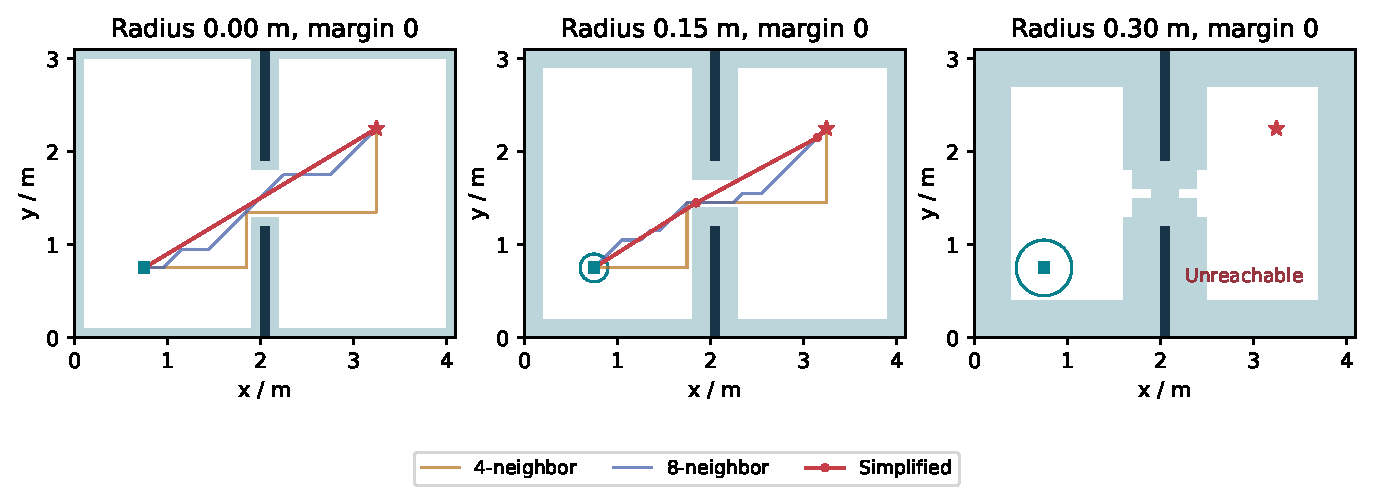
\includegraphics[width=\linewidth]{figures/ch11_astar.pdf}
\caption{深色是给定隔墙，浅蓝是额外阻塞的配置空间格子，白色可规划。
绿方块为起点，红星为目标；绿圆保持真实半径与坐标等比例。红线为八邻接结果的简化。}
\end{figure}
\begin{center}\small
\pgfplotstabletypeset[col sep=comma,
columns={radius,neighbors,status,grid_cost,expanded,simplified_points},
columns/radius/.style={column name=半径/m},columns/neighbors/.style={column name=邻接},
columns/status/.style={column name=状态,string type,string replace*={found}{找到},string replace*={unreachable}{不可达}},
columns/grid_cost/.style={column name=图代价/m,string type,string replace*={inf}{---}},
columns/expanded/.style={column name=扩展节点},columns/simplified_points/.style={column name=简化点数},
every head row/.style={before row=\toprule,after row=\midrule},
every last row/.style={after row=\bottomrule}]{data/ch11_astar.csv}
\end{center}
本实验裕量为零，半径分别为 0、0.15、0.30 m。四邻接成功时图代价为 4 m，
八邻接约为 3.12132 m。两种半径的成功代价相同不表示路径完全相同：栅格中可以存在多个等长路线。
扩展节点数同时受启发式、可用区域和并列排序影响，不能当作一般性能承诺。

0.7 m 门能在连续几何中容纳直径 0.6 m 的圆盘，但本例找不到整格都安全的贯通路径。
这是明确的离散保守性，不是把真实机器人偷偷变大；分辨率、半径与整格安全要求共同决定结果。
下一步接入观测地图后，还要区分几何变窄与尚未看见造成的封闭。

\begin{enumerate}
\item \textbf{理解：}在小网格上手算 $g,h,f$，解释四邻接与八邻接启发式的不同。
\item \textbf{代码：}完成邻居检查，覆盖外边界、两侧被挡和合法对角。
\item \textbf{实验：}改变半径、分辨率或未知策略，记录可达性、代价与简化点数。
\end{enumerate}
\textbf{验收：}30 组 seed=1111 随机栅格与独立 Dijkstra 的最短代价一致；
另检查已知四/八邻接距离、精确端点、同格路径、窄门、未知、外界、穿角、线段擦边/擦角与简化后安全。
ROS 观测地图和点击目标在下一功能接入。

\chapter{离障碍多远：二维距离场}
\begin{notebox}
\textbf{目标}\quad 从占据图构造距离场，推导任意位置的插值与梯度，并计算保守净空。\\
\textbf{先修}\quad 第 07、11 章的栅格、欧氏距离与碰撞几何。
\end{notebox}

\section{先看一个圆的距离场}
A* 回答“哪条路可以通行”。轨迹优化还希望知道：离障碍有多远，向哪个方向挪一点能增加间隙？
距离场给每个位置赋一个数，梯度则描述这个数增加最快的方向。
先运行一个有解析答案的圆形实验：
\begin{lstlisting}[language=bash]
ros2 run motion2d esdf_demo tmp/ch12_esdf
/usr/bin/python3 scripts/plot_ch12_esdf.py
\end{lstlisting}
半径为 1 m、圆心在原点的圆，其有符号距离为
\begin{equation}
d_{\rm circle}(x,y)=\sqrt{x^2+y^2}-1.
\end{equation}
圆外正、圆内负、边界零。例如 $(1.3,0)$ 距圆边 $.3$ m，$(.8,0)$ 距圆边向内 $.2$ m。
对平方根用链式法则，在 $(x,y)\neq(0,0)$ 处有
\begin{equation}
\frac{\partial d}{\partial x}=\frac{2x}{2\sqrt{x^2+y^2}},\qquad
\frac{\partial d}{\partial y}=\frac{2y}{2\sqrt{x^2+y^2}},\qquad
\nabla d=\frac{(x,y)^\top}{\sqrt{x^2+y^2}}.
\end{equation}
梯度朝圆外，长度为 1；移动小位移 $\Delta p$，距离变化约为 $\nabla d^\top\Delta p$。
圆心处所有径向方向都等价，而且沿 $x$ 轴的距离为 $|x|-1$，左右导数分别为 $-1,+1$，
所以那里没有唯一梯度。实验把这个圆离散成占据格，再研究离散场与解析圆之间的差别。

\section{格子中心距离与方格净空}
输入使用未膨胀的观测栅格。沿用上一章的标签策略：已观测且编码不超过 35 才自由，
未知默认阻塞；外围补一圈阻塞格，使靠近地图边界的位置也能感知外部空间。
记阻塞格中心集合为 $O_c$、自由格中心集合为 $F_c$，定义
\begin{equation}
d_i=\begin{cases}
\min_{c_j\in O_c}\|c_i-c_j\|,&i\text{ 自由},\\
-\min_{c_j\in F_c}\|c_i-c_j\|,&i\text{ 阻塞}.
\end{cases}
\end{equation}
自由位置寻找最近阻塞中心，阻塞位置寻找最近自由中心后加负号。
这样两侧的数值沿着“离开障碍”的方向增加，适合为优化提供移动方向。

中心之间的距离还包含方格本身的半个宽度。例如墙面位于 $x=0$，
紧邻墙面的阻塞中心位于 $-\rho/2$，自由中心位于 $+\rho/2$。
自由中心到墙的真实间隙为 $\rho/2$，到阻塞中心则为 $\rho$。
后面会将中心距离转换成到阻塞方格的保守下界。

\begin{center}
\begin{tikzpicture}[x=2cm,y=1cm,>=Stealth]
\fill[navy!12] (-1,-.45) rectangle (0,.45);
\draw[navy,thick] (0,-.55)--(0,.55);
\draw[->] (-1.15,0)--(1.15,0) node[right]{$x$};
\fill[navy] (-.5,0) circle(2pt);
\fill[tealblue] (.5,0) circle(2pt);
\node[below] at (-.5,-.2) {阻塞中心};
\node[below] at (.5,-.2) {自由中心};
\draw[<->] (-.5,.95)--(.5,.95) node[midway,above]{中心距 $\rho$};
\draw[<->] (0,1.7)--(.5,1.7) node[midway,above]{净空 $\rho/2$};
\draw[dotted] (-.5,.1)--(-.5,.85);
\draw[dotted] (.5,.1)--(.5,1.6);
\draw[dotted] (0,.6)--(0,1.6);
\end{tikzpicture}
\end{center}
整张地图阻塞时，自由中心集合为空，无法得到有限的内部距离；
代码用 $-\infty$ 标记，并让连续查询返回空结果。
整张地图自由时，外围阻塞圈仍提供种子，因此距离由外部边界决定。

\section{把二维最近距离拆成两次一维计算}
直接对每个格子枚举所有障碍中心，计算量会随格数和障碍数相乘增长。
欧氏距离变换（EDT）利用平方距离的结构来减少搜索。
先以格子索引为坐标，将种子格的代价设为 0，其余格设为 $+\infty$：
\begin{equation}
f(i,j)=\begin{cases}0,&(i,j)\text{ 是种子},\\+\infty,&\text{其他格}.
\end{cases}
\end{equation}
于是每个位置到最近种子的平方距离为
\begin{equation}
D(x,y)=\min_{i,j}\big[(x-i)^2+(y-j)^2+f(i,j)\big].
\end{equation}
这里的 $x,y,i,j$ 都是整数索引。非种子位置的无穷代价使它不会成为最小值。
对固定的 $i$，$(x-i)^2$ 与 $j$ 无关，可以提出内部最小值：
\begin{align}
A(i,y)&=\min_j[(y-j)^2+f(i,j)],\\
D(x,y)&=\min_i[(x-i)^2+A(i,y)].
\end{align}
第一式逐列计算上下距离，第二式逐行比较不同列的候选。
这是对所有候选做同一次最小化，只是改变了枚举顺序，结果保持一致。

例如种子在 $(0,0)$ 与 $(2,1)$，查询 $(1,2)$。
处理列后，第 2 行在列 $0,1,2$ 的值分别为 $4,+\infty,1$。
再加横向距离平方：$1+4,0+\infty,1+1$，最小值为 2，
对应种子 $(2,1)$。若 $\rho=.1$ m，则米制距离为 $.1\sqrt2$ m。
一般地，索引平方距离转为米制距离需要
\begin{equation}d=\rho\sqrt D.\end{equation}
以阻塞中心为种子做一次 EDT，以自由中心为种子再做一次，随后按原标签选择正负值。

\code{squaredDistanceTransform} 中的列循环与行循环正好对应 $A$ 和 $D$。

\section{一维距离变换：维护抛物线的最低部分}
\subsection{由平方距离得到抛物线交点}
两次一维处理都具有相同形式：给定数组 $f(q)$，求
\begin{equation}D(x)=\min_q[f(q)+(x-q)^2].\end{equation}
将每个有限的 $f(q)$ 画成曲线 $P_q(x)=f(q)+(x-q)^2$。
它是一条开口相同、顶点为 $(q,f(q))$ 的抛物线。
对每个 $x$ 取最低的一条，得到的曲线称为\textbf{下包络}。
列处理后的 $f(q)$ 可能是非零平方距离，因此需要这种一般形式。

按 $q$ 从小到大加入新曲线。设已经保留的末条曲线中心为 $v<q$，两条曲线相等时
\begin{align}
f(q)+x^2-2qx+q^2&=f(v)+x^2-2vx+v^2,\\
2(q-v)x&=f(q)+q^2-f(v)-v^2.
\end{align}
共同的 $x^2$ 消掉了，所以交点只有一个：
\begin{equation}s=\frac{f(q)+q^2-f(v)-v^2}{2(q-v)}.\end{equation}
两曲线之差为 $P_q(x)-P_v(x)=2(q-v)(s-x)$。
因为 $q-v>0$，$x<s$ 时新曲线较高，$x>s$ 时新曲线较低。
因此新加入的中心只会从某个分界点开始，在右边接替旧曲线。

\subsection{一次删除中间曲线的手算}
令 $f(0)=0,f(1)=4,f(2)=0$，有
$P_0=x^2$、$P_1=4+(x-1)^2$、$P_2=(x-2)^2$。
开始只保留 $P_0$。加入 $P_1$ 时，交点为 $(4+1)/2=2.5$，暂记它从 2.5 开始胜出。
加入 $P_2$ 时，它与 $P_1$ 的交点为 $(4-5)/2=-.5$，早于 $P_1$ 原来的胜出位置 2.5。
也就是说，$P_1$ 还没来得及低于 $P_0$，就已被 $P_2$ 压在上方，因此可删除。
随后比较 $P_2$ 与 $P_0$，交点为 $4/4=1$。
最终 $x\leq1$ 选 $P_0$，$x\geq1$ 选 $P_2$；在交点两者数值相同。

\begin{center}
\begin{tikzpicture}
\begin{axis}[width=.8\linewidth,height=5.2cm,xmin=-.4,xmax=2.4,ymin=0,ymax=6.1,
  xlabel={查询索引 $x$},ylabel={平方代价},grid=major,
  legend style={at={(.5,1.05)},anchor=south,legend columns=2,font=\small},
  tick label style={font=\small}]
\addplot[navy,domain=-.4:2.4,samples=80]{x^2};\addlegendentry{$P_0=x^2$}
\addplot[orange!85!black,dashed,domain=-.4:2.4,samples=80]{4+(x-1)^2};\addlegendentry{$P_1=4+(x-1)^2$}
\addplot[tealblue,domain=-.4:2.4,samples=80]{(x-2)^2};\addlegendentry{$P_2=(x-2)^2$}
\addplot[black,very thick,domain=-.4:1,samples=35]{x^2};\addlegendentry{下包络}
\addplot[black,very thick,domain=1:2.4,samples=35,forget plot]{(x-2)^2};
\addplot[muted,dotted,forget plot] coordinates{(1,0)(1,1)};
\end{axis}
\end{tikzpicture}
\end{center}

\subsection{数组如何保存这条下包络}
\code{sites} 保存仍可能最低的中心索引，\code{begin} 保存每条曲线开始胜出的横坐标。
第一条曲线从 $-\infty$ 开始。加入新中心时，若交点不晚于末条曲线的 \code{begin}，
就删除末条并继续向前比较；否则将新曲线和分界点放在末尾。

\par\noindent\begin{minipage}{\linewidth}
\lstinputlisting[language=C++,linerange={edt_envelope_begin-edt_envelope_end},
  includerangemarker=false]{../ros2_ws/src/motion2d/src/mapping/distance_transform.cpp}
\end{minipage}\par
\code{last} 指向有效数组的末端；\code{--last} 删除一个候选，
随后 \code{++last} 腾出新位置。无穷的输入在进入这个循环前跳过，因为它们永远不会取得有限最小值。
包络建好后，查询 $x=0,1,\ldots$，用一个只向右移动的指针找到对应曲线即可。

每个中心最多入栈一次、出栈一次，读取阶段的指针也只向右经过每个中心一次。
因此长度为 $n$ 的一维数组只需与 $n$ 成正比的工作量，写为 $O(n)$。
宽 $W$、高 $H$ 的地图，列处理为 $W$ 次 $O(H)$，行处理为 $H$ 次 $O(W)$，合计为 $O(WH)$。
这套方法由 Felzenszwalb 与 Huttenlocher 系统给出。\footnote{原始论文：
\href{https://theoryofcomputing.org/articles/v008a019/}{Distance Transforms of Sampled Functions}，2012，第2节。}
用上面的三条抛物线逐步填写 \code{sites} 和 \code{begin}，就能追踪循环中的删除与追加。

\section{从四个中心值插出任意位置的距离}
\subsection{从一维线性插值到双线性插值}
距离数组存的是格子中心样本。若左下中心的索引为 $(i,j)$，其米制坐标是
$(o_x+(i+\tfrac12)\rho,o_y+(j+\tfrac12)\rho)$。
因此查询点先换成中心索引坐标：
\begin{equation}
\xi=\frac{x-o_x}{\rho}-\frac12,\qquad\eta=\frac{y-o_y}{\rho}-\frac12.
\end{equation}
取 $i=\lfloor\xi\rfloor,j=\lfloor\eta\rfloor$，
$u=\xi-i,v=\eta-j$ 表示在四个中心围成的方块内横、纵方向走过的比例，均在 $[0,1]$ 内。
查询范围限定在最外围中心组成的闭矩形；位于最大索引处时，用最后一个插值块并取比例 1。

\begin{center}
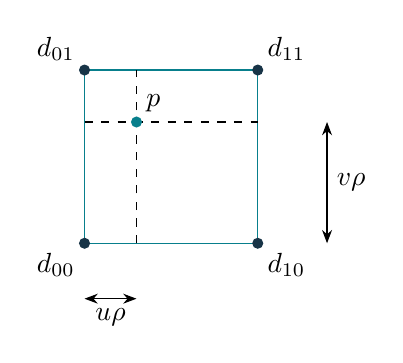
\begin{tikzpicture}[x=2.2cm,y=2.2cm,>=Stealth]
\draw[tealblue] (0,0) rectangle (1,1);
\foreach \x/\y/\label in {0/0/00,1/0/10,0/1/01,1/1/11} {
 \fill[navy] (\x,\y) circle(2pt);
}
\node[below left] at (0,0) {$d_{00}$};\node[below right] at (1,0) {$d_{10}$};
\node[above left] at (0,1) {$d_{01}$};\node[above right] at (1,1) {$d_{11}$};
\draw[dashed] (.3,0)--(.3,1);\draw[dashed] (0,.7)--(1,.7);
\fill[tealblue] (.3,.7) circle(2pt);\node[above right] at (.3,.7) {$p$};
\draw[<->] (0,-.32)--(.3,-.32) node[midway,below] {$u\rho$};
\draw[<->] (1.4,0)--(1.4,.7) node[midway,right] {$v\rho$};
\end{tikzpicture}
\end{center}
在一条线上，端点值为 $a,b$，满足两端值的直线是 $a+u(b-a)=(1-u)a+ub$。
所以先沿上下两行插值，再沿纵向插值：
\begin{align}
d_{\rm bottom}&=(1-u)d_{00}+ud_{10},\quad
 d_{\rm top}=(1-u)d_{01}+ud_{11},\\
\widetilde d&=(1-v)d_{\rm bottom}+v d_{\rm top}\\
&=(1-u)(1-v)d_{00}+u(1-v)d_{10}+(1-u)vd_{01}+uvd_{11}.
\end{align}
四个权重均非负，并且和为
$(1-v)[(1-u)+u]+v[(1-u)+u]=1$，所以插值值处于四个样本值的最小值与最大值之间。

\subsection{对权重求导，再换回米制坐标}
固定样本值，对 $u$ 求导，上下两行分别产生差值 $d_{10}-d_{00}$ 和 $d_{11}-d_{01}$；
对 $v$ 求导则得到上行值减下行值。
利用 $du/dx=dv/dy=1/\rho$，得到
\begin{align}
\frac{\partial\widetilde d}{\partial x}
&=\frac{(1-v)(d_{10}-d_{00})+v(d_{11}-d_{01})}{\rho},\\
\frac{\partial\widetilde d}{\partial y}
&=\frac{(1-u)(d_{01}-d_{00})+u(d_{11}-d_{10})}{\rho}.
\end{align}
距离单位为 m，坐标单位也为 m，因此梯度分量的单位为 m/m。
少除一次 $\rho$，就会把“走过一个格子时变化多少”误当成“走过一米时变化多少”。

\par\noindent\begin{minipage}{\linewidth}
\lstinputlisting[language=C++,linerange={esdf_bilinear_begin-esdf_bilinear_end},
  includerangemarker=false]{../ros2_ws/src/motion2d/src/mapping/esdf.cpp}
\end{minipage}\par
手算一个带交叉项的例子：以左下中心为局部原点，将米制坐标数值代入
$f(x,y)=2x+3y+xy$，取边长 $\rho=.2$。
四角值为 $0,.4,.6,1.04$；在 $u=.3,v=.7$ 处，局部坐标为 $(.06,.14)$，
插值值为 $.5484$，梯度为 $(2.14,3.06)$，与直接求导 $(2+y,3+x)$ 一致。
这也是 \textbf{代码练习 ch12-1} 的核对例子。

\subsection{怎样理解梯度的变化}
每个插值块内部可以直接使用上述导数；换到相邻块后，样本差值改变，梯度可能跳变。
在前面的直墙例子中，阻塞中心取 $-\rho$、自由中心取 $+\rho$，二者仅相距 $\rho$，
所以两中心之间插值的斜率为 $(\rho-(-\rho))/\rho=2$。
这说明本章的中心距离插值场可以提供平滑块内的移动方向，梯度长度则由离散样本决定。
代码原样保留这个导数，便于后面计算轨迹代价的链式梯度。

\section{从插值距离推导保守净空}
原始插值可能因样本间距和方格面积高估净空。
下面只用三角不等式，推导一个始终不大于地图实际间隙的数。
设四个插值中心都自由，记它们为 $c_k$，非负权重为 $w_k$，且 $\sum_k w_k=1$。

\subsection{移动一段距离，最近中心距离最多变化多少}
记 $d_c(p)$ 为查询点到最近阻塞中心的无符号距离。
假设 $c_*$ 是离 $q$ 最近的阻塞中心，那么
\begin{equation}
d_c(p)\leq\|p-c_*\|\leq\|p-q\|+\|q-c_*\|
=\|p-q\|+d_c(q).
\end{equation}
第一步是在所有中心中取最小值，第二步是三角不等式。
交换 $p,q$ 再写一次，就得到
\begin{equation}|d_c(p)-d_c(q)|\leq\|p-q\|.\end{equation}
这个性质称为 1-Lipschitz，直观上就是移动一米，最近距离至多改变一米。
特别地，每个中心样本给出下界 $d_c(p)\geq d_c(c_k)-\|p-c_k\|$。
乘以 $w_k$ 再相加，左边因权重和为 1 仍是 $d_c(p)$，于是
\begin{equation}
d_c(p)\geq\underbrace{\sum_k w_kd_c(c_k)}_{\widetilde d(p)}
-\underbrace{\sum_k w_k\|p-c_k\|}_{E(p)}.
\end{equation}
$E$ 是从四个中心插值到查询点时，为可能高估的距离预留的修正量。

\subsection{再把中心换成有面积的方格}
障碍格内任一点 $z$ 到格子中心 $c$ 的距离至多为半对角线
$h=\sqrt{(\rho/2)^2+(\rho/2)^2}=\rho/\sqrt2$。
又由三角不等式的变形，
\begin{equation}
\|p-z\|\geq\|p-c\|-\|z-c\|\geq d_c(p)-h.
\end{equation}
对所有阻塞方格中的 $z$ 取最小值，这个下界仍成立。
最近的地图外部点位于边界，外围阻塞圈的方格覆盖该边界，因此同一推导也包括地图外部。
将两个修正合在一起，并利用几何间隙非负，得到
\begin{equation}
\underline d(p)=\max\left(0,\widetilde d(p)-\sum_{k=1}^4 w_k\|p-c_k\|-\frac{\rho}{\sqrt2}\right).
\end{equation}
这对应 \code{EsdfSample::clearance_lower_bound}。
\code{sample} 先检查四个中心标签，再用四个双线性权重累加 \code{error}，
最后减去 \code{resolution/std::sqrt(2.)}。
若四个中心中包含阻塞格，采用零下界；零值表示当前计算还未给出正间隙，可继续用精确几何检查。

例如 $\rho=.2$ m，四角中心距离为 $(.6,.8,.6,.8)$ m，查询插值块中心。
四个权重都是 $1/4$，$\widetilde d=.7$ m，各角距离为 $.2/\sqrt2$ m，故
\begin{equation}
E=\frac{.2}{\sqrt2},\qquad
\underline d=.7-2\frac{.2}{\sqrt2}\approx.4172\ \text{m}.
\end{equation}
机器人半径 $.2$ m、裕量 $.05$ m 时，$.4172>.25$，这个中心位置满足间隙要求。
这里的下界针对当前占据方格所表达的几何；新观测修改地图后，需要相应重算距离场。

\subsection{三个返回值各自怎样使用}
\begin{center}\small
\begin{tabular}{lll}\toprule
字段 & 计算意义 & 后续用途\\\midrule
\code{distance} & 有符号中心距离的插值 & 构造避障代价\\
\code{gradient} & 上一项对 $x,y$ 的偏导 & 反传轨迹梯度\\
\code{clearance_lower_bound} & 到阻塞方格及外部的净空下界 & 检查圆心间隙\\\bottomrule
\end{tabular}
\end{center}
半径在这里通过 $\underline d>r+m$ 处理；输入用未膨胀地图，
而第十一章的配置空间地图已把半径计入，按中心点检查即可。
\code{gradient} 对应插值距离，计算下界时还额外减去了随位置变化的 $E$，所以两者导数不同。

对一条轨迹，检查一个位置只能确定这一处的间隙。
即使两个端点都有正距离，它们之间也可能穿过障碍。
第十三章将用安全凸区域包住一段路径，第十六章再利用曲线的控制点性质检查整段包含关系。

\section{用可以手算的场核对实现}
\begin{enumerate}
\item 从单个种子开始，枚举少量格子的距离平方，与两次一维 EDT 的中间数组逐项比较。
再试三条抛物线的删除例子，观察候选数组怎样缩短。
\item 给四角指定常数或双线性函数值，代入解析梯度，并用中心差分
$[d(p+\epsilon e_i)-d(p-\epsilon e_i)]/(2\epsilon)$ 核对。选取扰动前后都在同一插值块内的点。
\item 对几个轴对齐阻塞方格，用第七章的点到方格距离算出精确净空，
与 $\underline d$ 比较，并解释插值修正和半对角线修正各减掉了什么。
\end{enumerate}
这三组练习依次核对离散最小值、连续插值和面积修正，帮助区分不同来源的误差。

\section{分辨率实验与练习}
\begin{figure}[h]
\centering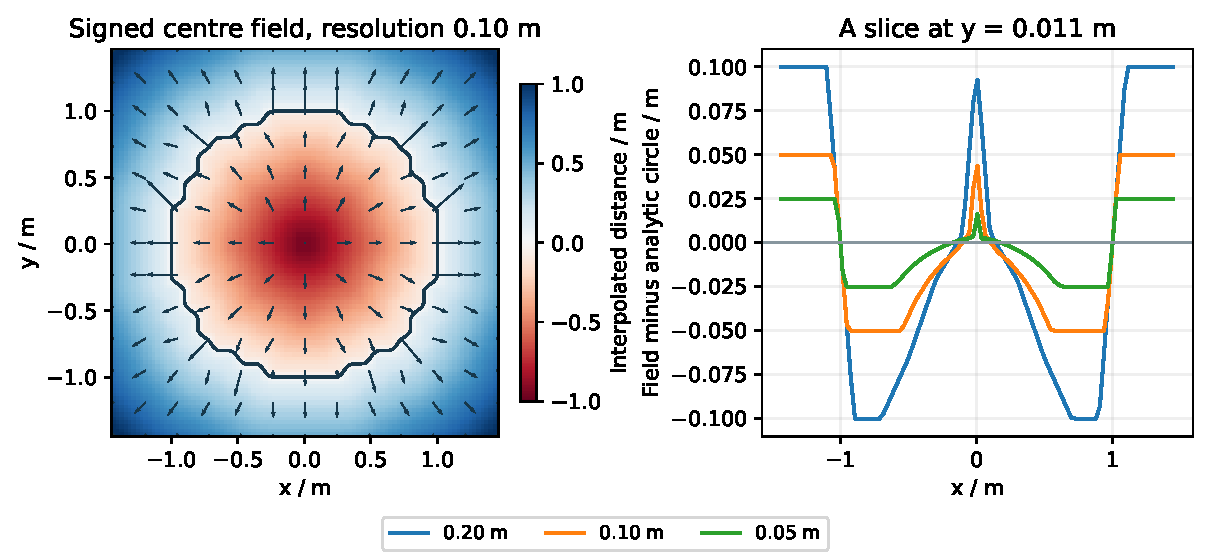
\includegraphics[width=.84\linewidth]{figures/ch12_esdf.pdf}
\caption{左：0.1 m 格的有符号场与插值梯度，坐标等比例。右：固定 y 的距离误差切片。
不同分辨率都存在栅格化和中心距离误差，靠近界面时插值也影响结果。}
\end{figure}
\begin{center}\small
\pgfplotstabletypeset[col sep=comma,
columns={resolution,cells,mae_m,max_error_m,median_us,p95_us},
columns/resolution/.style={column name=$\rho$/m,fixed,precision=2},columns/cells/.style={column name=格数},
columns/mae_m/.style={column name=平均误差/m,fixed,precision=4},
columns/max_error_m/.style={column name=最大误差/m,fixed,precision=4},
columns/median_us/.style={column name=中位数/$\mu$s,fixed,precision=1},
columns/p95_us/.style={column name=P95/$\mu$s,fixed,precision=1},
every head row/.style={before row=\toprule,after row=\midrule},
every last row/.style={after row=\bottomrule}]{data/ch12_esdf.csv}
\end{center}
给定地图为 $8\times8$ m；中心位于半径 1 m 圆内的格子标为占据。
三组都使用同一查询晶格，统计 $0.3\leq\|p\|\leq1.6$ m 环带内与解析圆距离的绝对误差。
这是栅格对圆的近似实验：一部分误差来自圆被方格表示，另一部分来自中心距离及插值。两种几何的边界位置也会随分辨率变化。
每个分辨率预热 5 次，计时 100 次，含分类、补边界和两个 EDT，不含 ROS 序列化。
表中更细网格的平均误差更小，构建时间更长。
分辨率减半时，每边格数约翻倍，二维总格数约变为四倍，正好可用来观察 $O(WH)$ 的规模变化。
每次保留相同查询点，误差才是在相同空间位置上比较。
单个位置可能因圆边落在不同格子内而出现误差波动。
平均绝对误差为 $N^{-1}\sum_i|\widetilde d(p_i)-d_{\rm circle}(p_i)|$，
最大误差则取这些绝对值中的最大者。100 次耗时排序后，表中的中位数取第 51 个，P95 取第 95 个，
分别反映一次典型运行和较慢运行的耗时。

\textbf{练习 ch12-1：}补全 bilinearGradient。给定
$f(x,y)=2x+3y+xy$ 在 $0,\rho$ 四角的值，验证 $\rho=0.2$ m、$u=0.3,v=0.7$ 时
梯度为 $(2.14,3.06)$。再验证常数场梯度为零。
推导题与代码提示见 \path{exercises/ch12}。

\textbf{理解与实验：}画解析圆场；解释圆心处不可微、中心距与边界距的差别。
改变分辨率，报告误差、格数和构建时间，保留相同查询点与计时范围。
常见错误是忘记开方、忘记乘分辨率、把索引坐标当米数，以及使用已经膨胀的地图再扣半径。
下面将距离场接入 ROS 可视化。

\section{ROS 距离通道与梯度显示}
\begin{lstlisting}[language=bash]
ros2 launch motion2d_bringup ch12.launch.py
ros2 topic echo /esdf/status
# In a separate terminal, with the same ROS_DOMAIN_ID:
/usr/bin/python3 scripts/check_ch12.py
/usr/bin/python3 scripts/plot_ch12_observed.py
\end{lstlisting}
esdf\_node 只订阅 /map，每张观测地图独立构建一个距离场。
本章启动沿用上一章的真值定位和激光观测建图；距离场的全部几何输入来自 /map。
输入与 A* 共用同一套自由阈值、未知策略和轴对齐地图验证，避免两者解释不同的地图。

\begin{center}\small
\begin{tabular}{lll}\toprule
话题 & 类型 & 语义 \\\midrule
/esdf/cloud & PointCloud2 & x、y、z、distance 四个 FLOAT32 \\
/esdf/gradients & MarkerArray & map 中的梯度方向箭头 \\
/esdf/status & String & ready / no\_finite\_field / invalid\_map \\\bottomrule
\end{tabular}
\end{center}
点云保持原地图的 width、height，按 $i=yW+x$ 行主序存储；每点 16 字节，
行步长为 $16W$。x、y 是格子中心的米制坐标，z 固定为零。
\textbf{distance 字段存有符号中心距离，单位 m}；z 用于点的位置高度，固定为零以便在平面上显示。
全阻塞时保留 $-\infty$ 并设置 is\_dense=false，同时发布 no\_finite\_field 和空箭头。
地图格式错误时清空点云与标记，不保留上一次的有效显示。

RViz 的 Color Transformer 选择 Intensity，Channel Name 选择 distance。
预设用 $[-0.5,2.0]$ m 固定颜色范围，超出范围只在显示颜色上饱和，消息里的数值不变。
Size (m) 默认匹配 0.1 m 分辨率；修改地图分辨率后应相应调整显示方块大小。
配置空间掩码、观测图与 ESDF 是不同产物，可在 Displays 中切换比较。

梯度默认每隔 10 格显示一个箭头，箭头方向朝距离增加处。
显示长度为 $\min(0.4,0.2\|\nabla\widetilde d\|)$ m，箭头头部随短箭头缩放；
例如梯度模长为 1 时画 $.2$ m 箭头，模长为 3 时按上限画 $.4$ m，便于在同一画面内比较方向。
\lstinputlisting[language=C++,linerange={esdf_arrow_begin-esdf_arrow_end},
  includerangemarker=false]{../ros2_ws/src/motion2d/src/nodes/esdf_node.cpp}
消息沿用地图时间戳与 map 系，QoS 保留最新场。时间回退后直接用新地图重建；
晚加入的 RViz 读取当前快照。

\clearpage
\section{读一次真实距离消息}
下图来自实际 ROS 的距离点云与箭头消息，固定为 reset 后 100 步、0.5 s。
图仅截取默认随机世界左下部分；负值同时包含占据、不确定和按策略阻塞的未知区域。
颜色不能代替原始占据图中的观测来源信息。

\begin{figure}[!ht]
\centering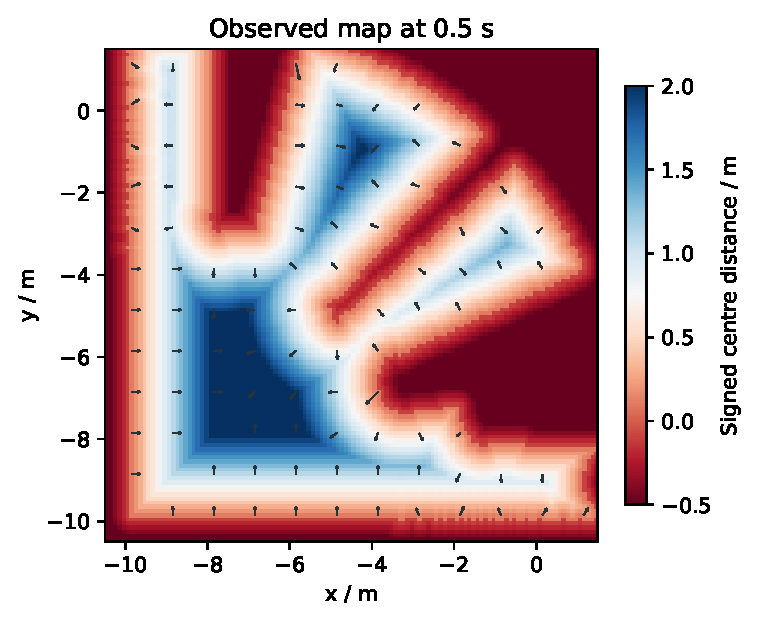
\includegraphics[width=.72\linewidth]{figures/ch12_observed.pdf}
\caption{实际观测距离场与消息中的梯度箭头。坐标为米且等比例，颜色在固定范围内显示。
图中箭头采用消息给定的位置与方向。}
\end{figure}

从地图中任选一个自由格，枚举所有阻塞中心及外围种子，手算其最近中心距离，
再读取点云同一索引的 \code{distance} 字段比较。
例如宽度为 220、索引 $(x,y)=(3,2)$，其点编号为 $2\times220+3=443$，
点起始字节为 $443\times16=7088$，distance 位于该点的第 12 字节偏移，因此从 7100 字节开始读取。
三个位置字段和一个距离字段均为四字节浮点数，所以每点合计 16 字节。

再分别输入全未知图与全自由图：全未知图缺少自由中心，显示不可用场；
全自由图仍可看到朝地图内部增大的正距离，因为外部补了一圈阻塞格。
将未知策略和颜色范围放在一起观察，可以理解同一颜色背后可能对应不同观测状态。

\textbf{消息练习：}
\begin{enumerate}
\item 从 /esdf/cloud 读取一格的四个字段，手算中心坐标和行字节偏移。
\item 把 esdf.gradient\_stride 从 10 改为 5，比较箭头密度，说明为何数值距离不变。
\item 对全自由小地图，解释为什么越靠近地图边界，正距离越小。
\end{enumerate}
独立检查入口、命令和评分见本章练习说明。

\chapter{让整段曲线有地方走：安全走廊}
\begin{notebox}
\textbf{目标}\quad 沿 A* 路径构建整块安全的凸区域，并为后续轨迹分配走廊和连接点。\\
\textbf{先修}\quad 第 11、12 章；凸集、线段与半平面。
\end{notebox}

\section{先比较矩形与凸多边形}
\begin{lstlisting}[language=bash]
ros2 run motion2d corridor_demo tmp/ch13_corridor
/usr/bin/python3 scripts/plot_ch13_corridor.py
\end{lstlisting}
本章先使用给定栅格隔离算法，输入是已经膨胀的配置空间和原始 A* 邻格折线。
实验路线从隔墙左下方绕到上端，再回到右下方。先得到一串相互交叠的局部矩形，
再尝试合并成较少的凸多边形；每次合并都重新检查整个区域。

\section{一个凸区域的两种表示}
顶点表示适合画图；半空间表示适合写约束。对逆时针多边形，边从 $a_i$ 指向 $a_{i+1}$，
内部在边的左侧。令 $e_i=a_{i+1}-a_i$，单位外法向为
\begin{equation}
n_i=\frac{(e_{iy},-e_{ix})^T}{\|e_i\|},\qquad
b_i=n_i^Ta_i,\qquad \mathcal C=\{p\mid A p\leq b\}.
\end{equation}
$A$ 的第 $i$ 行是 $n_i^T$，各行法向长度均为 1；故 $n_i^Tp-b_i$ 是到该边直线的带符号距离，单位 m。
它非正表示点在此半平面中。一个点必须满足所有行，才属于整个区域。
\lstinputlisting[language=C++,linerange={corridor_halfspace_begin-corridor_halfspace_end},
  includerangemarker=false]{../ros2_ws/src/motion2d/src/planning/corridor.cpp}

\begin{notebox}
\textbf{已经在配置空间内}\quad 走廊容纳的是机器人圆心，输入格子的半径和安全裕量已在第十一章处理。
这里不再次缩小一个物理半径。只有半空间约束正确且整个区域安全，才能使用后面的凸性论证。
\end{notebox}
公开接口为 makeRegion、regionIsFree 和 buildCorridor；结果同时保留顶点与半空间。
凸多边形须严格凸、逆时针且非退化。练习 ch13-1 从一条边写出对应的单位外法向和偏移。

\clearpage
\section{从局部矩形开始}
对每一段原始邻格路径，取起终点所在格子的包围框。若点恰好在格线或格角上，种子包含两侧格子。
框内每格都自由才可开始扩张，然后轮流尝试向左、右、下、上增加一条完整栅格边。
任何新增格被阻塞，就不接受这次扩张。每侧还有局部扩展长度限制 $L$，对应最多
$\lfloor L/\rho\rfloor$ 格；演示设置 $L=0.6$ m。
\lstinputlisting[language=C++,linerange={corridor_rectangle_begin-corridor_rectangle_end},
  includerangemarker=false]{../ros2_ws/src/motion2d/src/planning/corridor.cpp}
输出边界向内缩 $10^{-6}\rho$，在浮点运算下保留与阻塞格的分离。
每条种子线段的两个端点仍须在矩形内，所有边界约定与完整区域检查一致。
如果当前最后一个矩形已经包含下一段的两个端点，就无需重复添加。
扩张顺序会影响形状；这不是最大面积矩形求解器，合并后的区域也不再受单个种子的扩展窗口限制。

\section{安全顶点不足以证明区域安全}
一个四边形的四个顶点、甚至四条边都可能自由，而小障碍被包在正中间。
因此 regionIsFree 遍历区域包围框内的\textbf{阻塞方格}，求它们与走廊多边形的闭集交集。
只要交集非空，就拒绝；擦角或沿边接触也算非空。

实现对多边形逐次施加方格的四个半平面约束。跨越某个边界 $n^Tp=b$ 的边段，
设两端残差为 $\alpha=n^Tp_0-b$、$\beta=n^Tp_1-b$，交点为
\begin{equation}
p_\ast=p_0+\frac{\alpha}{\alpha-\beta}(p_1-p_0).
\end{equation}
保留半平面内的顶点与必要交点，重复四次。碰撞检查保留退化的点和线，避免漏掉接触。
地图外部也被拒绝。检查针对整块区域，不需要靠稠密采样猜测内部是否安全。

\section{只有通过验证才合并}
把相邻矩形顶点放在一起求凸包，再调用同一个 regionIsFree。
通过则替换成凸包，否则保留两个已有区域。转弯内侧的障碍经常导致合并失败，这是应保留的约束。
浮点近共线顶点若不满足严格凸性，也放弃该次可选合并。
局部矩形刻意有扩展窗口，因此在更大自由空间中，合并后可以出现六边形等非矩形区域。

\clearpage
\section{交叠区域决定连接点}
设相邻两个走廊为 $\mathcal C_i,\mathcal C_{i+1}$，先求交集
\begin{equation}
\mathcal I_i=\mathcal C_i\cap\mathcal C_{i+1}.
\end{equation}
它也由凸半平面裁剪得到。这里要求\textbf{正面积}，只共用一条边或一个点不够。
数值阈值为 $10^{-10}\rho^2$；这个阈值只排除退化交叠，实际运动余量仍受地图与半径决定。
从交集多边形的顶点 $v_1,\ldots,v_K$ 取平均作为连接点：
\begin{equation}
q_i=\frac1K\sum_{k=1}^K v_k.
\end{equation}
这是一个容易计算的内部点，不是多边形的面积质心，也不保证最大净空。
起点和终点采用原始请求坐标，最终 $N$ 个走廊对应 $N+1$ 个路点。
第 $i$ 条新线段的两个端点都属于 $\mathcal C_i$，于是由凸性有
\begin{equation}
(1-s)q_i+s q_{i+1}\in\mathcal C_i,\qquad 0\leq s\leq1.
\end{equation}
这证明的是\textbf{分配后的直线段}整段包含在安全区域。
经过相同路点的五次曲线可能向外鼓出，不能直接复用这条证明；第十六章会检查整段 Bezier 凸包。

\section{失败时不返回半成品}
\begin{center}\small
\begin{tabular}{ll}\toprule
状态 & 含义 \\\midrule
empty\_path & 没有可用路径 \\
unsafe\_path & 原始折线含越界、穿障或接触 \\
blocked\_seed\_box & 线段安全，但整格种子框不可用 \\
no\_positive\_overlap & 相邻区域没有正面积交叠 \\
invalid\_extension & 扩展长度参数不合法 \\\bottomrule
\end{tabular}
\end{center}
失败结果的区域和路点均为空，调用方应保留明确失败状态。
尤其不要把贪心简化后的长对角线直接拿来扩张矩形：线段可以绕过方格，包围框却可能覆盖它。
保留原始 A* 邻格路径更适合本章构造方式；已有长线段可另行重新离散搜索。

验证覆盖单位法向、几何包含、点/线退化交叠、内部障碍、擦边/擦角、非矩形安全凸包、
转弯路线与不同栅格尺度。对每个最终区域验证整块无碰撞，并检查分配给它的两个端点。
这些是地图所表达的几何证书，仍依赖观测质量与定位质量。

\clearpage
\section{固定地图上的对照实验}
\begin{figure}[h]
\centering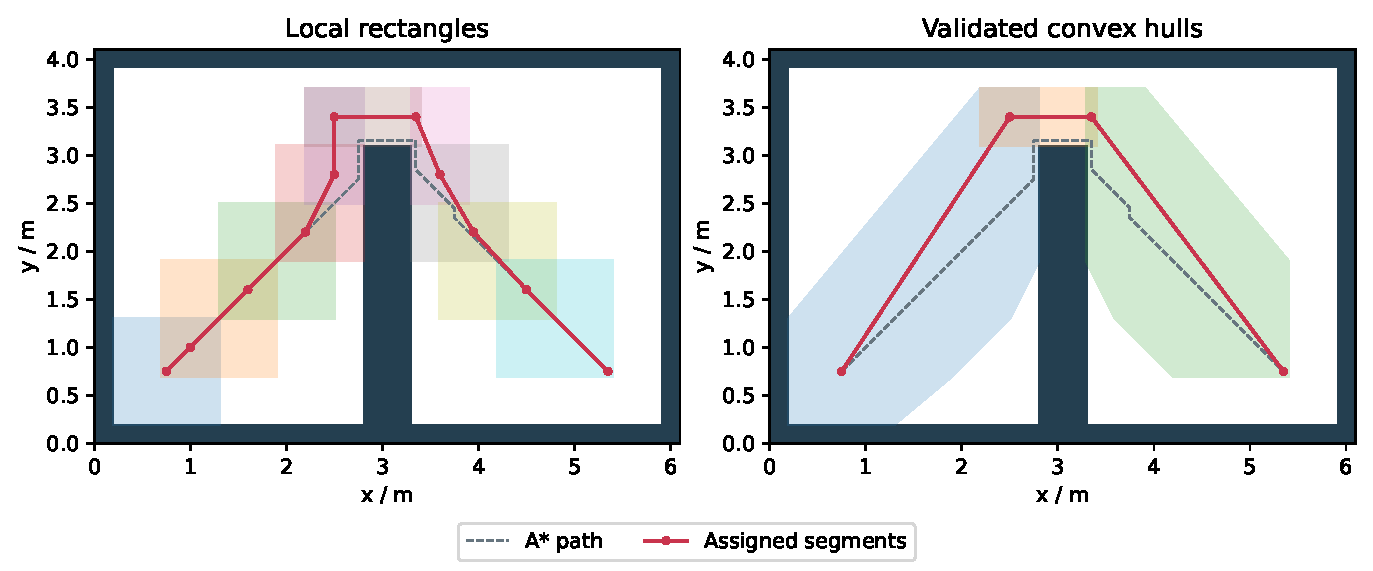
\includegraphics[width=\linewidth]{figures/ch13_corridor.pdf}
\caption{深色为已膨胀阻塞格，浅色为走廊，虚线为原始 A* 路径。
红色线段的两个端点均分配到同一个凸区域中。两图采用相同坐标比例。}
\end{figure}
\begin{center}\small
\pgfplotstabletypeset[col sep=comma,
columns={convex,regions,vertices,waypoints,min_overlap_area_m2},
columns/convex/.style={column name=凸包合并,string type,string replace*={0}{关},string replace*={1}{开}},
columns/regions/.style={column name=区域数},columns/vertices/.style={column name=总顶点数},
columns/waypoints/.style={column name=路点数},
columns/min_overlap_area_m2/.style={column name=最小交叠/$m^2$,fixed,precision=3},
every head row/.style={before row=\toprule,after row=\midrule},
every last row/.style={after row=\bottomrule}]{data/ch13_corridor.csv}
\end{center}
给定图为 $61\times41$ 格，分辨率 0.1 m，半径 0.15 m，额外裕量为零。
隔墙上端留出绕行空间，起终点分别为 $(0.75,0.75)$、$(5.35,0.75)$ m。
在完全相同的 A* 路径上，局部矩形为 10 个，安全凸包合并后为 3 个；总顶点数从 40 变成 19。
两种构造的最小交叠面积都约为 $0.06\,m^2$，所以连接点没有落在仅共边的退化位置。

区域变少会减少后续轨迹分段和约束的组织成本，但不代表最短路径、最小 jerk 或最大走廊体积。
本章没有给红线分配时间，也没有直接驱动机器人。

\begin{enumerate}
\item \textbf{理解：}画一个内部含障碍的凸四边形，说明只测顶点和边会遗漏什么。
\item \textbf{代码 ch13-1：}把 CCW 边转为单位半空间。底边 $(1,2)\to(4,2)$ 给出 $-y\leq-2$；
斜边 $(4,2)\to(7,6)$ 的外法向为 $(0.8,-0.6)$。
\item \textbf{实验：}改变局部扩展长度与合并开关，记录区域数、形状与最小交叠面积。
保持地图、半径和路径相同，解释变化原因。
\end{enumerate}
ROS 观测路径上的走廊显示将在下一功能接入。

\chapter{给路径加上时间：五次轨迹}
\begin{notebox}
\textbf{目标}\quad 从端点位置、速度、加速度推导五次曲线，理解分段时间与解析采样，再接入理想执行。\\
\textbf{先修}\quad 第 04、11、13 章；多项式求导、链式法则与线性方程。
\end{notebox}

\section{同样走一米，为什么感觉不同}
几何路径只说经过哪里；轨迹还要说何时到达、到达时多快。
先从静止出发，沿 $x$ 轴走 1 m 后静止，分别用 2 s 和 4 s 完成：
\begin{lstlisting}[language=bash]
ros2 run motion2d quintic_demo tmp/ch14_quintic
/usr/bin/python3 scripts/plot_ch14_quintic.py
\end{lstlisting}
图中的位置曲线走过相同距离，较慢的一组将变化摊到更长时间里，因此速度和加速度更小。
下面从端点条件构造这些曲线，并直接对多项式求导，得到任意时刻的速度和加速度。

\begin{figure}[!ht]
\centering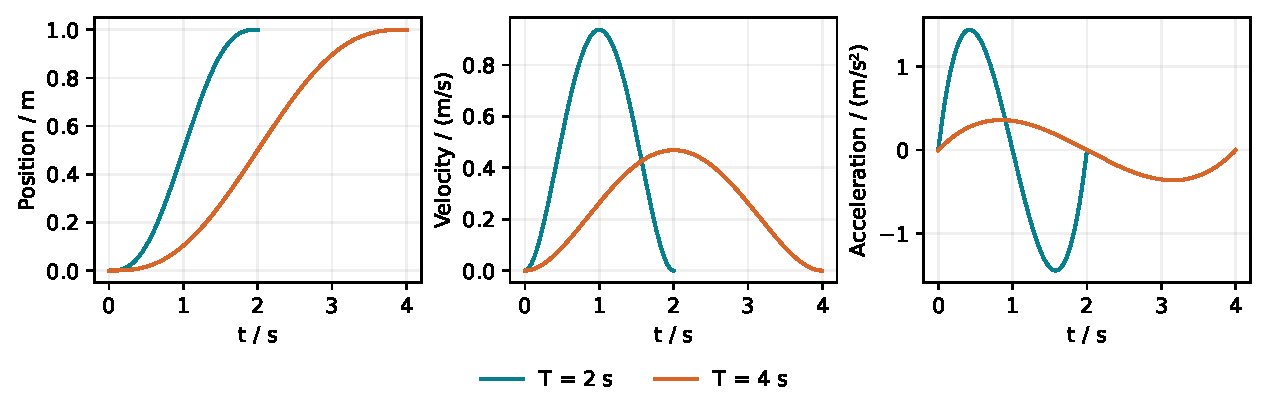
\includegraphics[width=\linewidth]{figures/ch14_scaling.pdf}
\caption{同一几何线段的时间缩放。时长翻倍，速度缩为一半，加速度缩为四分之一。}
\end{figure}

\section{六个边界条件怎样确定六个系数}
\subsection{先用归一化时间写边界}
起点与终点各给位置、速度、加速度，共六个标量条件。
有六个系数的五次多项式正好可以容纳这组条件。二维时对两个坐标分别求解，时长 $T>0$ 共用：
\begin{equation}
p(t)=\sum_{k=0}^{5}c_k t^k,\qquad
\dot p(t)=\sum_{k=1}^{5}kc_k t^{k-1},\qquad
\ddot p(t)=\sum_{k=2}^{5}k(k-1)c_k t^{k-2}.
\end{equation}
$c_k$ 是二维列向量，单位为 $\mathrm{m}/\mathrm{s}^k$。
令 $s=t/T$，将同一条曲线写为 $p(t)=P(s)=\sum_{k=0}^5 b_k s^k$。
$s$ 无量纲，$b_k$ 的单位均为 m；展开 $(t/T)^k$，可知 $c_k=b_k/T^k$。
对时间求导还需用链式法则：
\begin{equation}
\dot p(t)=\frac1T P'(s),\qquad
\ddot p(t)=\frac1{T^2}P''(s).
\end{equation}
因此在 $s=0$ 的三个条件依次给出
\begin{equation}b_0=p_0,\qquad b_1=Tv_0,\qquad b_2=\tfrac12T^2a_0.\end{equation}
在 $s=1$，目标则为 $P(1)=p_1,P'(1)=Tv_1,P''(1)=T^2a_1$。
把已知的前三项移到右边，记剩余量为
\begin{align}
r_0&=p_1-b_0-b_1-b_2,\\
r_1&=Tv_1-b_1-2b_2,\qquad r_2=T^2a_1-2b_2.
\end{align}
三个剩余未知量满足
\begin{equation}
\begin{aligned}
b_3+b_4+b_5&=r_0,\\
3b_3+4b_4+5b_5&=r_1,\\
6b_3+12b_4+20b_5&=r_2.
\end{aligned}
\end{equation}
这些等式对 $x$、$y$ 坐标逐分量成立，可以把向量当作两组相同系数的方程来计算。

\subsection{逐步消元得到代码里的组合}
第二行减去第一行的三倍，第三行减去第一行的六倍，得到
\begin{equation}
b_4+2b_5=r_1-3r_0,\qquad
6b_4+14b_5=r_2-6r_0.
\end{equation}
再用后一式减去前一式的六倍：
$2b_5=r_2-6r_1+12r_0$。回代先求 $b_4$，再求 $b_3$：
\begin{equation}
\begin{aligned}
b_5&=6r_0-3r_1+\tfrac12r_2,\\
b_4&=-15r_0+7r_1-r_2,\\
b_3&=10r_0-4r_1+\tfrac12r_2.
\end{aligned}
\end{equation}
消元时只除以固定非零数，所以任意有限的六个边界值都确定唯一的一组归一化系数。
正时长使最后的 $T^{-k}$ 转换有定义。

\par\noindent\begin{minipage}{\linewidth}
\lstinputlisting[language=C++,linerange={quintic_boundary_begin-quintic_boundary_end},
  includerangemarker=false]{../ros2_ws/src/motion2d/src/trajectory/quintic.cpp}
\end{minipage}\par
代码先填 $b_0,b_1,b_2$，再计算三个残差并回代；最后的 \code{power} 依次取 $1,T,T^2,\ldots,T^5$，
将各列转成秒制系数 $c_k$。
\code{interpolateQuintic} 接收两端的 \code{TranslationState}，返回一个 \code{QuinticPiece}：
正时长加 $2\times6$ 系数矩阵，第一行表示 $x$，第二行表示 $y$，列按\textbf{升幂}排列。

\section{对同一个多项式求各阶导数}
对单项 $c_k t^k$ 求 $r$ 次导数，每次幂次减一，并把原幂次乘到前面：
\begin{equation}
p^{(r)}(t)=\sum_{k=r}^5
\underbrace{k(k-1)\cdots(k-r+1)}_{r\text{ 个因子}}c_k t^{k-r}.
\end{equation}
$r=0$ 时乘积取 1，恢复位置；$r=1,2,3$ 分别为速度、加速度、jerk（加速度的变化率）。
jerk 单位为 $\mathrm{m/s^3}$。高于五阶的导数为零，本章接口接受 0 到 5 阶。

计算多项式可用 Horner 法：从高次项向低次项，反复“乘时间，再加下一系数”。
例如 $d_0+d_1t+d_2t^2+d_3t^3=d_0+t[d_1+t(d_2+td_3)]$。
求导后的系数也可以这样排列，所以同一个循环能计算所有阶数：

\par\noindent\begin{minipage}{\linewidth}
\lstinputlisting[language=C++,linerange={polynomial_derivative_begin-polynomial_derivative_end},
  includerangemarker=false]{../ros2_ws/src/motion2d/src/trajectory/polynomial.cpp}
\end{minipage}\par
内层循环得到上式的 $r$ 个因子，外层从第 5 列往第 $r$ 列走。
最后得到的最低幂是 $t^0$，所以循环在 $k=r$ 时结束。
例如 $x(t)=1+2t+3t^2+4t^3$，则
$\dot x=2+6t+12t^2$、$\ddot x=6+24t$；在 $t=.5$ s，位置为 3.25 m，速度为 8 m/s，加速度为 18 $\mathrm{m/s^2}$。
\textbf{代码练习 ch14-1} 用这个例子核对幂次和乘数。

秒制系数已经包含了 $T^{-k}$，采样器直接代入本段的秒数。
若使用归一化系数 $b_k$ 求导，才需要再按链式法则乘 $T^{-r}$。
两种表示得到同一状态，选择一种约定贯穿保存、发送和采样即可。

\section{静止到静止：形状与峰值都可以手算}
\subsection{从系数得到单调的线段运动}
令 $\Delta p=p_1-p_0$，两端速度与加速度均为零，则 $b_1=b_2=0$、$r_0=\Delta p,r_1=r_2=0$。
代入消元结果便有
\begin{equation}
p(t)=p_0+\Delta p\,h(s),\qquad
h(s)=10s^3-15s^4+6s^5,\quad s=t/T.
\end{equation}
逐次求导并整理：
\begin{align}
h'(s)&=30s^2-60s^3+30s^4=30s^2(1-s)^2,\\
h''(s)&=60s-180s^2+120s^3=60s(1-s)(1-2s),\\
h'''(s)&=60(1-6s+6s^2).
\end{align}
由 $h'(s)\geq0$、$h(0)=0,h(1)=1$，可知 $h$ 在区间内单调从 0 增到 1。
因此位置始终是 $p_0,p_1$ 的非负加权平均，整段保持在线段上。
若该线段属于上一章的安全凸走廊，这种静止到静止的时间分配保持同样的几何包含关系。

\subsection{从导数为零的位置求峰值}
记线段长度 $D=\|\Delta p\|$。速度模长为 $D h'(s)/T$。
极值候选满足 $h''=0$，即 $s=0,1/2,1$；
两端速度为零，中点 $h'(1/2)=30/16=15/8$，所以
\begin{equation}v_{\rm peak}=\frac{15D}{8T}=1.875\frac DT.\end{equation}
加速度模长为 $D|h''|/T^2$。在正、负两半分别寻找极值，令 $h'''=0$：
\begin{equation}
6s^2-6s+1=0\quad\Longrightarrow\quad s=\frac{3\pm\sqrt3}{6}.
\end{equation}
这两点满足 $s(1-s)=1/6$、$|1-2s|=1/\sqrt3$，代入便有
\begin{equation}a_{\rm peak}=\frac{10\sqrt3}{3}\frac D{T^2}.\end{equation}
jerk 的归一化因子 $h'''=360(s-1/2)^2-30$ 在区间内介于 $-30$ 与 60，
故其模长最大值在两端取得：
\begin{equation}j_{\rm peak}=60\frac D{T^3}.\end{equation}
例如 $D=1$ m、$T=2$ s，三个峰值分别为 $.9375$ m/s、$1.4434$ $\mathrm{m/s^2}$、$7.5$ $\mathrm{m/s^3}$。
它们可以直接与第一幅图和后面的实验表核对。

若要为这一特殊线段设置上限 $v_{\max},a_{\max},j_{\max}>0$，将三条峰值不等式分别对 $T$ 求解：
\begin{equation}
T\geq\max\left(\frac{15D}{8v_{\max}},
\sqrt{\frac{10\sqrt3 D}{3a_{\max}}},
\sqrt[3]{\frac{60D}{j_{\max}}}\right).
\end{equation}
这给出了一个可直接实现的时长分配练习。重复点 $D=0$ 时，用正的最短时长生成原地停留段。

\subsection{时间缩放的适用条件}
保持 $P(s)$ 不变，将时长从 $T$ 改为 $\lambda T$，第 $r$ 阶物理导数缩为原来的 $\lambda^{-r}$。
因此时长翻倍时，速度、加速度、jerk 分别乘 $1/2,1/4,1/8$。
这里比较的是\emph{同一归一化形状}。静止边界自动满足这个条件。
若保持非零的物理边界速度 $v_0$ 不变，却重新改变 $T$，则 $b_1=Tv_0$ 也改变，
整条曲线形状可能随之改变；这时应重新求系数后比较。

\section{把若干段接成连续轨迹}
\subsection{连续性是连接处的条件}
把第 $i$ 段终点和第 $i+1$ 段起点设为同一组 $(p,v,a)$，
就使位置、速度与加速度的左极限和右极限相等，称为 $C^2$ 连续。
各段内部是光滑多项式；连接处的 jerk 是否相等，还要比较两边的三阶导数。
例如一维逐点停靠的两段 $0\to1\to3$ m，时长都为 2 s：
连接处两边 $v=a=0$，但左侧 jerk 为 $60\times1/2^3=7.5$，右侧为 $60\times2/2^3=15$ $\mathrm{m/s^3}$。
速度和加速度可以连续，jerk 同时发生跳变。



\code{PolynomialTrajectory} 在相邻段处比较位置、速度、加速度，分别采用对应 SI 单位的 $10^{-7}$ 绝对容差。
最简单的 \code{stopAtWaypoints} 在每个路点设 $v=a=0$，并分配
\begin{equation}
T_i=\max\left(T_{\min},\frac{\|q_{i+1}-q_i\|}{v_{\rm nom}}\right).
\end{equation}
$v_{\rm nom}$ 表示用来计算时长的平均速度参数；在距离项起作用时，峰值为 $1.875v_{\rm nom}$。
每个中间点停下便于观察分段和碰撞几何。第十五、十六章将调整内部速度与加速度，使运动更加连贯。

\begin{figure}[!ht]
\centering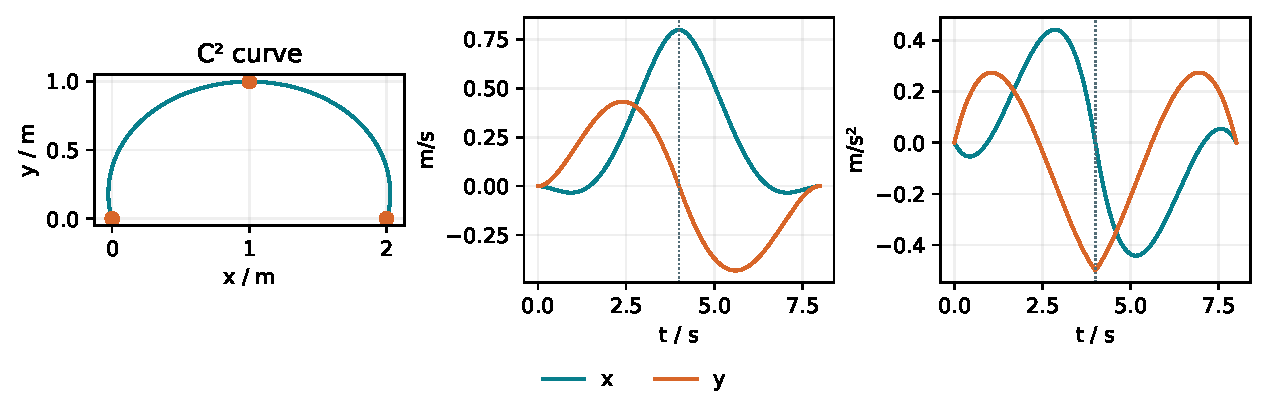
\includegraphics[width=\linewidth]{figures/ch14_join.pdf}
\caption{两个 4 s 分段，连接点 $(1,1)$ m，连接速度 $(0.8,0)$ m/s、加速度 $(0,-0.5)$ $\mathrm{m/s^2}$。
虚线是连接时刻；图形坐标等比例，速度与加速度连续。}
\end{figure}

\subsection{绝对时间、轨迹时间与单段时间}
设绝对开始时刻为 $t_0$，收到查询时刻 $t_{\rm sim}$，先算整条轨迹时间 $\tau=t_{\rm sim}-t_0$。
再减去前面各段时长，得到第 $i$ 段局部时间：
\begin{equation}t_i=\tau-\sum_{k<i}T_k.\end{equation}
多项式 $c_0+c_1t_i+\cdots+c_5t_i^5$ 只接受本段的 $t_i$。
例如 $t_0=.203$ s，两段时长为 $.458,.637$ s，连接与结束时刻为 $.661,1.298$ s。
在仿真时刻 $.700$ s，$\tau=.497$ s，应查询第二段的 $t_2=.039$ s。

\begin{center}
\begin{tikzpicture}[x=6.5cm,y=1cm,>=Stealth]
\draw[->] (0,0)--(1.44,0) node[right]{$t_{\rm sim}$};
\draw[tealblue,very thick] (.203,0)--(.661,0);
\draw[navy,very thick] (.661,0)--(1.298,0);
\foreach \x/\lab in {.203/.203,.661/.661,1.298/1.298} {
 \draw (\x,-.08)--(\x,.08);\node[below] at (\x,-.12){$\lab$ s};
}
\node[font=\small] at (.432,.42){第1段：$T_1=.458$ s};
\node[font=\small] at (.98,.42){第2段：$T_2=.637$ s};
\draw[orange!85!black,->] (.700,.9)--(.700,.08);
\node[above] at (.700,.9){查询 $.700$ s：$t_2=.039$ s};
\end{tikzpicture}
\end{center}
内部连接时刻选择右段，最终时刻选择末段终点。
代码在累计结束时间数组中用 \code{upper_bound} 找第一个严格大于查询时间的边界，正好实现这条规则。
$p,v,a$ 在连接处相同，而 jerk 按所选段给出明确的单侧值。
轨迹前后如何等待与保持，由执行器在下面统一处理。
\subsection{解析参考与显示折线}
/plan/trajectory\_path 是稀疏采样预览：总头记录发布时间，每个 PoseStamped 记录未来执行时间。
真正执行始终使用完整系数；预览折线的密度不影响仿真精度。
RViz 中可同时观察洋红色参考、圆盘与实际轨迹。把预览采样间隔调大，会看到折线变粗糙，
但接收端在同一时刻求出的多项式状态保持一致。


\clearpage
\section{保存系数并复现采样结果}
演示输出 samples.csv、summary.csv 和 coefficients.csv。
系数文件逐行保存案例、段号、时长、坐标轴与六个升幂系数，可用相同采样器重建；不包含 yaw。
平移参考与 yaw 分开指定。全向机器人可以向侧面运动，同时保持机头方向；
阿克曼模型的朝向与速度方向关系已在第四章推导，其轨迹规划在第十六章接入。

\begin{center}\small
\pgfplotstabletypeset[col sep=comma,
columns={case,duration,peak_speed,peak_acceleration,peak_jerk},
columns/case/.style={column name=案例},columns/duration/.style={column name=总时长/s},
columns/peak_speed/.style={column name=速度/(m/s), fixed,precision=4},
columns/peak_acceleration/.style={column name=加速度/(m/s$^2$), fixed,precision=4},
columns/peak_jerk/.style={column name=jerk/(m/s$^3$), fixed,precision=4},
every head row/.style={before row=\toprule,after row=\midrule},
every last row/.style={after row=\bottomrule}]{data/ch14_quintic.csv}
\end{center}
每条完整轨迹在 $t_n=nT_{\rm total}/2000$、$n=0,\ldots,2000$ 处采样，
表中列出这些样本的最大模长。案例 0、1 是上面的 1 m 静止线段，三个解析峰值都可以用来比较采样误差。
例如加速度极值落在 $s=(3\pm\sqrt3)/6$，通常位于两个采样点之间；增加采样密度会更接近它。
案例 2 使用图中的非零连接导数。读取系数文件重新采样，比较连接时刻的左右极限，
再用中心差分检查任意一段内部的解析导数。

\begin{enumerate}
\item \textbf{推导：}从六个静止端点约束推导 $h(s)$，说明 $T$ 翻倍后的各阶导数缩放。
\item \textbf{代码 ch14-1：}完成升幂系数的一阶、二阶导数；避免重复时间缩放。
\item \textbf{实验：}修改中间点速度，比较曲线形状与连续性；解释为何路点安全不足以证明曲线安全。
\end{enumerate}
\section{把轨迹作为完整消息发送}
\begin{lstlisting}[language=bash]
ros2 launch motion2d_bringup ch14.launch.py
ros2 topic pub --once /goal_pose geometry_msgs/msg/PoseStamped \
  '{header: {frame_id: map}, pose: {position: {x: -7.5, y: -8.0}, orientation: {w: 1.0}}}'
ros2 service call /trajectory/execute std_srvs/srv/Trigger '{}'
ros2 topic echo /sim/trajectory_status
\end{lstlisting}
先等待扫描建图与目标规划成功，再调用服务。
点击目标负责产生几何路线；调用服务将当前路线转换为一次完整执行。
trajectory\_node 从区域连接路径取得几何点，从 /odometry 取得选定的定位结果，并用 TF 统一坐标。

motion2d\_interfaces 用分段消息保存系数、用整条轨迹消息保存执行时间和朝向：
\begin{center}\small
\begin{tabular}{ll}\toprule
Trajectory2D 字段 & 明确语义 \\\midrule
header & 发布时间；执行坐标系固定为 odom \\
start\_time & 仿真时钟上的绝对执行起始时刻 \\
pieces & 非空五次分段；每段 duration、x[6]、y[6] \\
yaw & 独立常值朝向，单位 rad \\\bottomrule
\end{tabular}
\end{center}
每段系数以局部秒升幂存储；时长必须有限且为正，连接需满足 $C^2$。
消息转换逐项复制系数与时长，接收端因此能在任意时刻计算参考。
例如 start\_time=0 表示从仿真原点开始；start\_time=.75 s 表示在时钟到达 .75 s 时开始。

\section{把 map 路线固定到 odom}
执行节点在当前里程计时刻查询 $^{odom}T_{map}$，转换所有路点，然后求逐点停靠轨迹。
发布时固定这次变换，整条执行参考随后在 odom 中保持一致。
设转换为 $p_o=Rp_m+d$，若 map 中已有多项式系数，则
\begin{equation}c^o_0=Rc^m_0+d,\qquad c^o_k=Rc^m_k\quad(k\geq1).\end{equation}
因为平移 $d$ 与时间无关，只进入常数项；旋转对每一阶向量都作用相同。
本章代码先变换路点再插值，也得到相应的 odom 曲线。在线重规划与回环衔接将在第十九章处理。
\par\noindent\begin{minipage}{\linewidth}
\lstinputlisting[language=C++,linerange={trajectory_publish_begin-trajectory_publish_end},
  includerangemarker=false]{../ros2_ws/src/motion2d/src/nodes/trajectory_node.cpp}
\end{minipage}\par
\code{transformPoint} 对应点的刚体变换；\code{stopAtWaypoints} 生成各段系数，
\code{lead_} 换成纳秒后加到当前时刻，设置未来的开始时间。
默认平均速度 0.4 m/s、最短分段 0.5 s，执行起点比发布时间晚 0.25 s。
若路线起点与当前位置不一致，拒绝发布并等待新路线；运动中再次发送轨迹由本章执行器明确拒绝。
服务成功表示已发布，最终接收结果看 /sim/trajectory\_status。

\section{用解析参考驱动理想模型}
\subsection{等待、执行与保持}
选择 \code{model=trajectory} 后，仿真器从 /plan/trajectory 接收完整曲线。
这条理想运动分支直接令状态等于参考 $p,v,a$，可先集中观察规划几何和传感器时间。
接收时要求曲线起点与当前位姿一致，两端 $v=a=0$，yaw 连续，开始时刻尚未过去。
这些条件把运动平滑地接到静止等待与终点保持：
\begin{equation}
p_{\rm held}(\tau)=\begin{cases}
p(0),&\tau<0,\\p(\tau),&0\leq\tau\leq T_{\rm total},\\p(T_{\rm total}),&\tau>T_{\rm total}.
\end{cases}
\end{equation}
区间外 $v=a=0$；区间内使用曲线导数。两端的零导数使这条整体参考达到 $C^2$ 连续。
暂停会停止仿真时钟，reset 清空曲线并回到初始状态。
后面的惯性模型将把同样的参考交给控制器，由力与力矩推动机器人接近它。

\subsection{由系数得到步内加速度上界}
仿真每次推进一个时间步，需要检查两端之间的弯曲运动。
第四章已由两次积分推导：若步长为 $h$、步内 $\|\ddot p\|\leq a_{\max}$，
曲线与端点连线之间的偏差不超过
\begin{equation}\delta=\frac{a_{\max}h^2}{8}.\end{equation}
现在曲线是多项式，可以直接从系数求 $a_{\max}$。
对本段局部区间 $0\leq t\leq t_{\max}$，逐项用三角不等式，再利用非负幂的单调性：
\begin{align}
\|\ddot p(t)\|&=\left\|\sum_{k=2}^5 k(k-1)c_k t^{k-2}\right\|\\
&\leq\sum_{k=2}^5 k(k-1)\|c_k\|t^{k-2}
\leq\sum_{k=2}^5 k(k-1)\|c_k\|t_{\max}^{k-2}.
\end{align}
各项单位均为 $\mathrm{m/s^2}$。把向量模长分别相加会忽略项间抵消，所以结果可高于实际峰值，
但整个区间的加速度都被覆盖。一个时间步跨过连接点时，对涉及的每段分别求界，然后取最大值。

\par\noindent\begin{minipage}{\linewidth}
\lstinputlisting[language=C++,linerange={polynomial_sweep_begin-polynomial_sweep_end},
  includerangemarker=false]{../ros2_ws/src/motion2d/src/trajectory/execution.cpp}
\end{minipage}\par
\code{offset} 是当前段在整条轨迹中的起始时间；\code{hi} 将查询终点转换到该段局部时间，
并限制在段末。\code{power} 依次是 $1,t_{\max},t_{\max}^2,t_{\max}^3$，恰好对应加速度中的四项。

例如从 0 到 1 m 的 2 s 静止曲线，非零系数为 $c_3=1.25,c_4=-.9375,c_5=.1875$。
局部时刻不超过 1 s 时，上界为 $7.5+11.25+3.75=22.5$ $\mathrm{m/s^2}$。
取一个长 5 ms、结束不晚于 1 s 的仿真步，得到
$\delta=22.5\times.005^2/8\approx7.03\times10^{-5}$ m。
于是用半径 $r+\delta$ 的圆盘沿端点连线扫掠，就包含原半径 $r$ 沿曲线扫过的全部位置。

\subsection{先确定可推进的时间，再生成传感器样本}
扫掠检查通过后，才接受这次状态推进，并在其中各个传感器采样时刻求解析状态。
检测到碰撞风险时，保持上一个有效状态、冻结时钟，状态为 \code{collision_predicted}。
传感器因此也停在已经接受的时间范围内。
这一步由仿真世界执行，承担物理碰撞裁判的作用；规划仍使用前面建立的观测地图。

\clearpage
\section{在传感器自己的时刻采样}
\begin{lstlisting}[language=bash]
# 默认ch14在运行时
/usr/bin/python3 scripts/check_ch14.py
/usr/bin/python3 scripts/plot_ch14_execution.py
# 停止上一个launch，再运行独立空房间时间实验
ros2 launch motion2d_bringup ch14.launch.py rviz:=false \
  config:=$PWD/ros2_ws/src/motion2d_bringup/config/ch14_time_lab.yaml
/usr/bin/python3 scripts/check_ch14_time.py
\end{lstlisting}

\begin{figure}[!ht]
\centering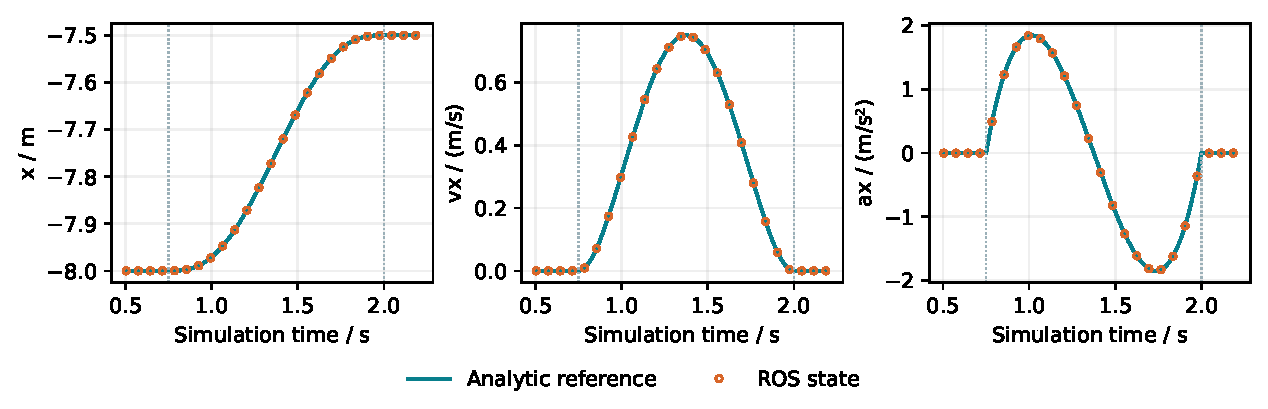
\includegraphics[width=\linewidth]{figures/ch14_execution.pdf}
\caption{实际观测地图上执行半米路线。0.75 s 开始、2 s 结束；实测 p/v/a 与解析参考重合，
用空心点区别采样结果与参考曲线。}
\end{figure}

第一组在真值定位的观测地图上规划 $(-8,-8)\to(-7.5,-8)$ m。
reset 后至 .5 s 发布目标，以默认平均速度 $.4$ m/s 分配时长，得到 $T=.5/.4=1.25$ s。
加上 $.25$ s 提前量，开始与结束时刻便是 $.75$ s 和 $2$ s。
将这些数代入静止线段公式，就能画出图中的参考，并逐条与 ROS 状态消息比较。

第二组用空房间与零噪声，选择 yaw=.4 rad、90 束、137 Hz IMU 和 7 Hz 雷达。
两段轨迹开始、连接、结束时刻为 $.203,.661,1.298$ s，均位于 5 ms tick 之间。
传感器周期也与 tick 不整除：第 29 个 IMU 周期对应
$t=29/137\approx.211678832$ s，它位于 $.210$ 与 $.215$ s 之间。
按前面的时间转换，应在第一段局部 $t_1\approx.008678832$ s 处计算加速度。
随后按第六章的旋转和重力项生成机体系比力，按第五章的射线模型生成雷达距离。

只修改时间戳而沿用 tick 末端状态，会给这个样本代入晚了约 $.003321168$ s 的加速度。
用一个便于手算的局部函数 $x(t_1)=t_1^3$（系数单位 $\mathrm{m/s^3}$）说明：
$\ddot x=6t_1$，上述时差产生约 $.019927$ $\mathrm{m/s^2}$ 的误差。
对一般轨迹，短时误差约为 $j\Delta t$，来自加速度的一阶泰勒展开。
可见采样时刻同时决定消息时间戳和消息数值。

\textbf{练习：}
\begin{enumerate}
\item 用时间实验脚本生成的系数重建 $.700$ s 的第二段状态，确认局部时间为 $.039$ s。
\item 取一条非整步 IMU 消息，分别用采样时刻与 tick 末端时刻求比力，比较差值。
\item 在空房间中发送穿墙曲线，观察最后接受的时刻、碰撞状态，以及之后的消息数量。
解释为何冻结物理时间后，传感器也应停止产生更晚的样本。
\end{enumerate}
进一步的消元、峰值、时间缩放与代码练习见 \path{exercises/ch14}。

\chapter{让路点之间更平顺：二维 MINCO}
\begin{notebox}
\textbf{目标}\quad 给定路点和时长求最小 jerk 曲线，把系数代价传回路点与时长。\\
\textbf{先修}\quad 第 14 章；矩阵方程、链式法则，本章补充必要的最优化条件。
\end{notebox}

\section{相同路点、相同时长的比较}
\begin{lstlisting}[language=bash]
ros2 run motion2d minco_demo tmp/ch15_minco
/usr/bin/python3 scripts/plot_ch15_minco.py
\end{lstlisting}
上一章在每个路点停下，易于构造，但未选择合适的中间速度和加速度。
本章固定路点 $q_i$ 与分段时长 $T_i>0$，保留两端的 p/v/a，求解整个区间的
\begin{equation}
\min J=\sum_{i=1}^{N}\int_0^{T_i}\|p_i'''(t)\|^2\,dt.
\end{equation}
jerk 是加速度的变化率。$J$ 常被称为控制能量，这里单位是 $\mathrm{m^2/s^5}$，不是物理焦耳。
MINCO 是一种利用路点和时长确定最小控制代价轨迹的表示；课程根据
\href{https://arxiv.org/html/2103.00190v4}{作者论文}中的最优性思想，独立实现固定二维、五次、最小 jerk 子问题。

\begin{figure}[!ht]
\centering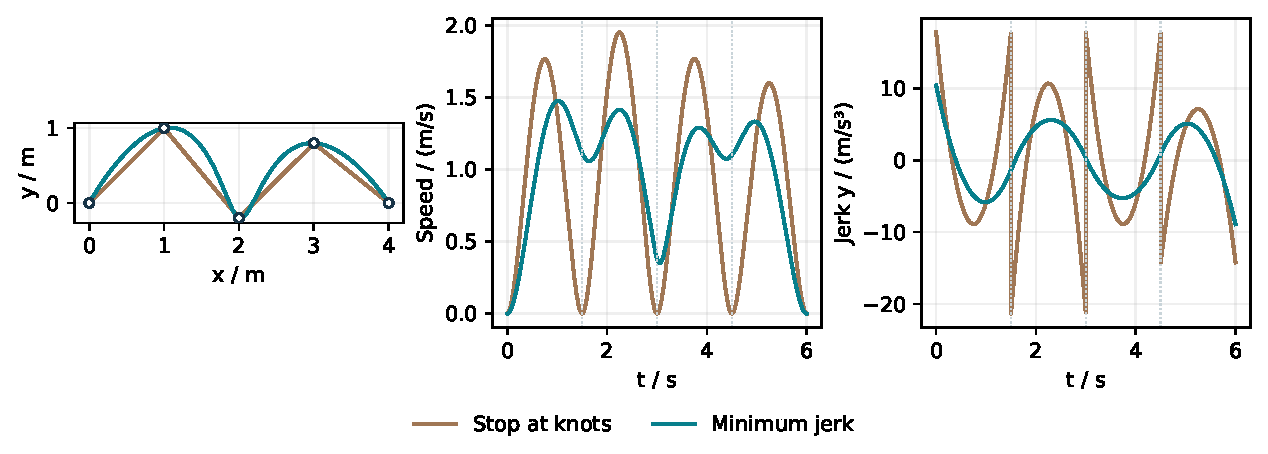
\includegraphics[width=\linewidth]{figures/ch15_minco.pdf}
\caption{四段均为 1.5 s。圆点是固定路点，虚竖线是连接时刻。
最小 jerk 解允许内部点有非零速度，连接处 jerk 连续；此图没有施加避障约束。}
\end{figure}

\section{能量是系数的二次型}
将单段系数按升幂排成 $C\in\mathbb R^{6\times2}$，则 $J_i=\operatorname{tr}(C^TQ(T_i)C)$。
$Q$ 只有第 3 到 5 次项对应的部分非零；对 $k,l\geq3$，
\begin{equation}
Q_{kl}(T)=\frac{k(k-1)(k-2)\,l(l-1)(l-2)}{k+l-5}T^{k+l-5}.
\end{equation}
这只是先求导、相乘再积分；代码 jerkGram 没有数值积分误差。
练习 ch15-1 用单段 $J=720\|p_1-p_0\|^2/T^5$ 检查因子与幂次。

\section{为什么最优解还要连续 jerk 与 snap}
只要求 p/v/a 连续时，内部速度和加速度仍可调整。
让曲线发生一个小变化 $\delta p$，对 $\delta J=2\int p'''\cdot\delta p'''dt$ 做三次分部积分，得到
\begin{equation}
\frac{\delta J}{2}=\left[p'''\cdot\delta p''-p''''\cdot\delta p'
+p'''''\cdot\delta p\right]_0^T-\int_0^T p^{(6)}\cdot\delta p\,dt.
\end{equation}
每段内部变化任意，故最优解满足 $p^{(6)}=0$，即至多五次。
在固定位置的内部路点处 $\delta p=0$，而两侧共享的 $\delta v,\delta a$ 可以自由变化。
相邻段端点项的符号相反，因此它们的系数必须抵消：jerk 与 snap 分别连续。
合上原有 p/v/a 连续，便得到 $C^4$；第五阶导数仍可跳变。

\section{将最优性写成一组线性方程}
每段六个系数，每个坐标共 $6N$ 个未知数。方程数量恰好也是 $6N$：
\begin{itemize}
\item 首尾各三个 p/v/a 条件，共 6 行。
\item 每个内部连接：jerk、snap 连续各一行，左段终点固定位置一行，p/v/a 连续三行，共 6 行。
\end{itemize}
把二维系数堆为 $C\in\mathbb R^{6N\times2}$，一次求解两个右端项：
\begin{equation}
A(T)C=B(q).
\end{equation}
每一行只涉及相邻两段，所以按代码顺序排列后，上下带宽均为 6。
\lstinputlisting[language=C++,linerange={minco_conditions_begin-minco_conditions_end},
  includerangemarker=false]{../ros2_ws/src/motion2d/src/trajectory/minco2d.cpp}
insert 将对应阶导数的基函数系数放入矩阵；例如零时刻 jerk 对 $c_3$ 的系数是 6。
矩阵约束已经包含最优性，求解阶段无需再迭代下降能量。trajectory() 返回上一章的统一采样对象。

\clearpage
\section{系数随路点和时长一起变化}
以后添加避障或速度代价，先计算它们对系数、时长的\textbf{直接偏导}。
记 $G=\partial K/\partial C$、$g_T=\partial K/\partial T$；固定系数时，jerk 代价有
\begin{equation}
G_i=2Q(T_i)C_i,\qquad (g_T)_i=\|p_i'''(T_i)\|^2.
\end{equation}
但是改变 $T_i$ 后，保持边界条件需要重新求系数；只保留这个非负上限项，会丢掉关键变化。
例如单段静止到静止的完整导数为 $dJ/dT=-3600\|\Delta p\|^2/T^6$，反而是负值。

对 $AC=B$ 求微分，得到 $A\,dC=dB-(dA)C$。
为了避免对每个路点单独求一次 $dC$，先求一个\textbf{伴随方程}：
\begin{equation}
A^T\Lambda=G,\qquad
 dK=\langle\Lambda,dB-(dA)C\rangle+g_T^T dT.
\end{equation}
$\langle X,Y\rangle=\sum_{ij}X_{ij}Y_{ij}$ 表示逐项乘积求和。
一个路点只改变 $B$ 对应的一行；故直接取该行 $\Lambda$。
某一时长只改变其所在段的右端导数值；再对时间求导，阶数增加一阶。
\lstinputlisting[language=C++,linerange={minco_adjoint_begin-minco_adjoint_end},
  includerangemarker=false]{../ros2_ws/src/motion2d/src/trajectory/minco2d.cpp}
中间连接对应的导数阶数为 $[4,5,1,1,2,3]$，与上一页六行方程逐一对应；
最后一段仅有末端 p/v/a，使用 $[1,2,3]$。
energyPartials 给出直接偏导；propagate 输出总路点/时长梯度，也能处理未来其他可微代价。

\section{为什么不用显式矩阵求逆}
代码先将 $A$ 分解为 $LU$，正向求解先解 $Ly=B$、再解 $UC=y$。
伴随复用同一组因子，先解 $U^Ty=G$、再解 $L^T\Lambda=y$。
固定带宽下，每行只读写常数个邻居，储存、分解和每次求解都随段数线性增长。
这指算法复杂度；实际速度对照在第十六章测量。

\clearpage
\section{带状实现和数值尺度}
\lstinputlisting[language=C++,linerange={band_factor_begin-band_factor_end},
  includerangemarker=false]{../ros2_ws/src/motion2d/src/trajectory/banded_lu.cpp}
BandedLu 只保存每行附近 13 个元素。教学实现使用本章特定顺序的无主元 LU，
不是任意矩阵的通用稳定求解器。若主元非有限或绝对值小于 $10^{-14}$，明确报告数值失败。
正时长保证数学问题可解，不保证任意悬殊尺度下的浮点计算稳定；优先使用秒、米和适中的分段时长。

\section{独立检查比看图更可靠}
测试另建一个密集等式约束二次型：只约束位置和 p/v/a 连接，不加入 jerk/snap 连续条件。
jerk 平方积分用三点 Gauss--Legendre 求积计算，它对该四次被积式精确。
将能量的驻点条件与等式约束联立为密集线性系统（KKT），求解后与带状结果比较，
避免用同一组最优性方程自证。
1--6 段、seed=1515 的小问题，系数相对误差门限为 $2\times10^{-9}$，连接到四阶检查门限为 $10^{-8}$。

对路点和时长采用步长 $10^{-5}$ 的中心差分，检查完整伴随梯度；
测试还增加系数平方与显式时长平方项，避免只验证 jerk 这个特殊目标。
允许误差为 $2\times10^{-6}\max(1,|g_{\mathrm{FD}}|)$，不是用差分替代实现中的解析梯度。

\begin{center}\small
\pgfplotstabletypeset[col sep=comma,
columns={mode,energy,peak_speed,peak_acceleration},
columns/mode/.style={column name=模式,string type,string replace*={0}{逐点停靠},string replace*={1}{MINCO}},
columns/energy/.style={column name=jerk 积分, fixed,precision=3},
columns/peak_speed/.style={column name=速度峰值, fixed,precision=3},
columns/peak_acceleration/.style={column name=加速度峰值, fixed,precision=3},
every head row/.style={before row=\toprule,after row=\midrule},
every last row/.style={after row=\bottomrule}]{data/ch15_minco.csv}
\end{center}
演示两端为 $(0,0),(4,0)$ m，中间为 $(1,1),(2,-0.2),(3,0.8)$ m，首尾静止。
四段各 1.5 s；能量是解析积分，速度/加速度峰值来自 3001 个采样点。
本次能量降低，曲线也偏离折线；\textbf{没有施加障碍、走廊或动力学约束}。

\begin{enumerate}
\item \textbf{推导：}为什么只固定内部位置，最优解仍有连续 jerk 与 snap？
\item \textbf{代码 ch15-1：}完成 jerkGram 的一个条目，检查低次项为零、积分指数和因子。
\item \textbf{实验：}固定相同边界、路点和时长，对比能量；改变一段时长检查解析梯度的符号与数值。
\end{enumerate}
本章下一功能将加入正时长参数化、软约束优化与独立的可行性检查。

\chapter{换一种消元顺序：二维 Spline2D}
\begin{notebox}
\textbf{目标}\quad 理解块三对角系统，验证同一最小 jerk 问题的系数与梯度，实测性能。\\
\textbf{先修}\quad 第 14、15 章；本章固定二维五次，不扩展到任意阶通用框架。
\end{notebox}

\section{先固定问题，再比较实现}
\begin{lstlisting}[language=bash]
ros2 run motion2d spline_demo tmp/ch16_spline
bash scripts/benchmark_ch16.sh
/usr/bin/python3 scripts/plot_ch16_spline.py
\end{lstlisting}
第一条无需下载。第二条是可选上游对照，使用
\href{https://github.com/Bziyue/SplineTrajectory}{SplineTrajectory} 的 QuinticSplineND<2>，固定版本为
\texttt{126525e49a43b0548bc6960e4979dd6b6258f289}。
上游为 MIT 许可证；对照脚本只在临时目录读取它，课程核心独立实现。
本章的 Spline2D 和上一章 MINCO 解决\textbf{同一个 clamped 最小 jerk 问题}：
相同首尾 p/v/a、内部位置和正时长，结果应相同。它不是另一条曲线，也不是把路点当 B-spline 控制点。

\section{未知数改为连接点的速度与加速度}
单段边界状态写为 $W_i=[p_i,v_i,a_i,p_{i+1},v_{i+1},a_{i+1}]^T$，每行有 x/y 两列。
第十四章已能从边界状态求六个系数，因此存在 $C_i=E_i(T_i)W_i$。
用单位边界依次调用 interpolateQuintic，可以直接构造 $E_i$ 的六列；无需初学者先抄一大组公式。
代入 jerk 二次型：
\begin{equation}
 J_i=\operatorname{tr}(W_i^TR_iW_i),\qquad R_i=E_i^TQ_iE_i.
\end{equation}
所有位置固定，首尾 v/a 固定，只有内部 $z_k=[v_k,a_k]^T$ 待求。
每段只含相邻两个节点，所以驻点条件形成对称块三对角系统：
\begin{equation}
 \begin{bmatrix}H_0&B_1^T&0\\B_1&H_1&B_2^T\\0&B_2&H_2\end{bmatrix}
 \begin{bmatrix}z_0\\z_1\\z_2\end{bmatrix}
 =\begin{bmatrix}r_0\\r_1\\r_2\end{bmatrix}.
\end{equation}
每个块为 $2\times2$，右端项有 x/y 两列。这是结构示例，实际块数为 $N-1$。
从各段 $R_i$ 取出对应 v/a 行列相加，已知位置和边界贡献移至右侧。

\clearpage
\section{一个块接一个块消元}
令 $D_0=H_0$，依次计算
\begin{equation}
 L_i=B_iD_{i-1}^{-1},\qquad D_i=H_i-L_iB_i^T.
\end{equation}
先解下三角，再解对角块，最后回代。每步固定规模，内存与时间随段数线性增长。
代码只对 $2\times2$ 正定块用 Cholesky 求解两个单位右端，缓存其逆作用；未显式求整张大矩阵的逆。
\lstinputlisting[language=C++,linerange={spline_blocks_begin-spline_blocks_end},
 includerangemarker=false]{../ros2_ws/src/motion2d/src/trajectory/spline2d.cpp}
得到所有节点 v/a 后，再经 $E_iW_i$ 还原为通用五次轨迹。
非正时长、维度不匹配、非有限数值或非正定分解均明确失败。任意悬殊时长仍可能损害浮点精度。

\section{能量梯度可以直接看边界}
第十五章分部积分给出的边界项也能用于梯度。内部位置的导数为两段第五阶导数之差：
\begin{equation}
 \frac{dJ}{dq_i}=2\left(p_{i-1}^{(5)}(T_{i-1})-p_i^{(5)}(0)\right).
\end{equation}
每段时长导数可在该段起点计算：
\begin{equation}
 \frac{dJ}{dT_i}=-\|p_i'''\|^2+2p_i''''\cdot p_i''-2p_i^{(5)}\cdot p_i'.
\end{equation}
这是固定端点、路点的\textbf{完整}导数；最优内部导数的变化因驻点条件消去。
把起点导数代成 $v=c_1,a=2c_2,j=6c_3,s=24c_4,p^{(5)}=120c_5$：
\lstinputlisting[language=C++,linerange={spline_energy_gradient_begin-spline_energy_gradient_end},
 includerangemarker=false]{../ros2_ws/src/motion2d/src/trajectory/spline2d.cpp}
该专用路径无需额外伴随。若加入 ESDF 等其他代价，仍需下一节的一般传播。

\clearpage
\section{任意代价的伴随如何复用块分解}
记未知内部导数为 $z$，其能量驻点条件为 $F(z,q,T)=0$，且 $F_z=H$。
给定系数偏导 $G_i$，先计算边界偏导 $E_i^TG_i$，累加得到 $K_z$。
再解 $H\lambda=K_z$，因此
\begin{equation}
 dK=K_q\,dq+K_T\,dT-\lambda^T(F_q\,dq+F_T\,dT).
\end{equation}
这里 $K_q,K_T$ 是固定 $z$ 的直接偏导。propagate 复用构造时的块分解求伴随。
为了计算 $E_T$，令 $M(T)C=W$ 为六个端点条件；由 $E=M^{-1}$ 得
$E_T=-EM_TE$。$M_T$ 只有末端三行非零，分别是速度、加速度、jerk 基函数。
然后对 $R=E^TQE$ 用乘积法则；这几步均为每段固定大小矩阵，仍是线性复杂度。

\section{误差验收与本机计时}
测试固定 seed=1616，1--12 段、非零边界 v/a、不同正时长。
系数与 MINCO 的相对误差要求低于 $10^{-9}$；MINCO 已另与独立密集 KKT 对照。
解析能量梯度与通用伴随交叉检查；含速度/加速度软惩罚的一般传播用 $10^{-5}$ 中心差分检查。

\begin{figure}[!ht]
\centering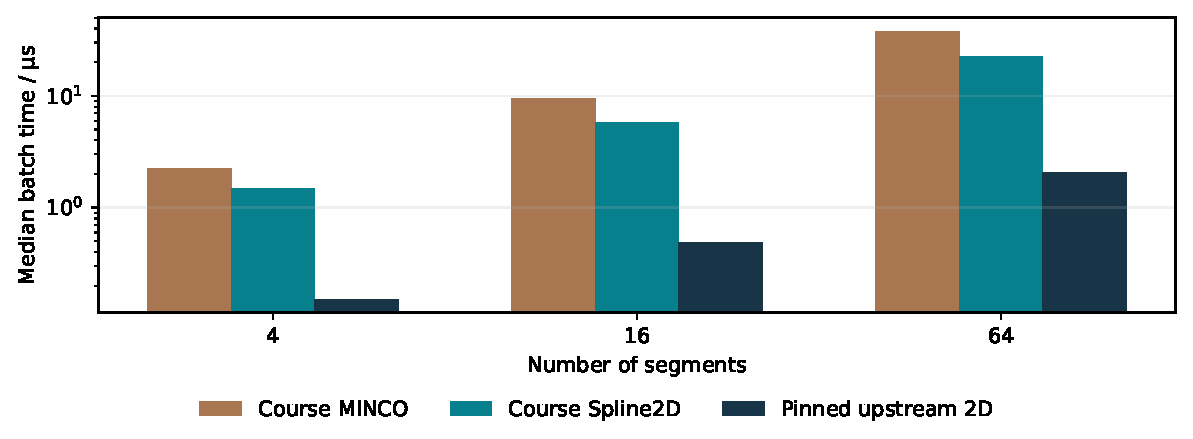
\includegraphics[width=\linewidth]{figures/ch16_comparison.pdf}
\caption{同一进程、相同输入下的构造、能量及完整能量梯度总耗时；纵轴为对数。
不包含地图、碰撞检查、I/O、ROS 或外层非线性优化。}
\end{figure}

\begin{center}\small
\begin{tabular}{rrrr}\toprule
段数 & 教学 MINCO/$\mu$s & 教学 Spline2D/$\mu$s & 固定上游/$\mu$s\\\midrule
4 & 2.247 & 1.476 & 0.152\\
16 & 9.453 & 5.793 & 0.484\\
64 & 38.000 & 22.735 & 2.049\\\bottomrule
\end{tabular}
\end{center}
GCC 15.2、Eigen 3.4、C++17，统一 -O3、-fno-fast-math，无 LTO；预热 10 次，21 组各 20 次，取组均值中位数。
同问题系数相对误差低于 $4.2\times10^{-14}$，能量梯度低于 $6.5\times10^{-13}$。
教学实现保留较多矩阵运算便于阅读；上游采用专门化公式。本机小实验不能替代完整规划器基准，也不承诺固定加速比。

\begin{enumerate}
\item \textbf{理解：}两种实现消去了不同变量，为何仍得到同一条曲线？
\item \textbf{代码 ch16-1：}补全 Schur 块，和独立 $4\times4$ 密集方程的解比较。
\item \textbf{实验：}改变段数与时长尺度，同时报告数值误差、失败状态及耗时，禁止只展示更快的一次。
\end{enumerate}

\chapter{让有质量的机器人跟上轨迹}
\begin{notebox}
\textbf{目标}\quad 从参考 p/v/a 计算真实力与力矩，区分反馈、前馈、模型失配和饱和。\\
\textbf{先修}\quad 第 04、14 章；本章参考已给定，先隔离跟踪问题。
\end{notebox}
\section{位置不是受力模型的控制量}
\begin{lstlisting}[language=bash]
ros2 run motion2d pd_tracking_demo tmp/ch17_pd
/usr/bin/python3 scripts/plot_ch17_pd.py
\end{lstlisting}
理想执行直接取参考位置。有质量的机器人满足 $m\dot v=F-c_vv$，
即使立刻改变力，速度和位置也不会瞬间跳到目标。
控制器从同一 odom 坐标系读取当前位置/速度及参考 p/v/a，先求期望加速度，再换算成力：
\begin{equation}
 e_p=p_r-p,\qquad e_v=v_r-v,\qquad
 F=\hat m(a_r+K_pe_p+K_de_v)+\hat c_vv.
\end{equation}
帽子表示控制器使用的参数估计；它不应悄悄读取模拟器真值参数。
$a_r$ 是前馈：提前提供沿曲线运动所需的加速度。
位置项把偏离拉回，速度项减小来回振荡；$K_p$ 单位为 s$^{-2}$，$K_d$ 为 s$^{-1}$。

\section{独立 yaw 与执行器限幅}
yaw 误差使用最短包角差，角速度误差按 rad/s 计算；再用转动惯量和角阻力换算力矩。
本章圆盘可全向受力，yaw 不决定平移方向；差速轮式车是另一种动力学模型。
\lstinputlisting[language=C++,linerange={pd_force_begin-pd_force_end},
 includerangemarker=false]{../ros2_ws/src/motion2d/src/control/pd_tracker.cpp}
trackPd 同时返回 requested 和 applied，方便看出要求了多少、实际执行了多少。
每个力轴分别限制在 $[-F_{\max},F_{\max}]$，力矩同理；没有把状态速度硬裁掉。
若力饱和，机器人可能跟不上轨迹，轨迹应减速或重新分配时间。

\clearpage
\section{固定参考后，比较原因而非只看最终位置}
实验使用空 8 m 方形边界、半径 0.2 m 圆盘；净空由边界到圆盘外缘的距离计算，
仅用于评估，不输入控制器。实际质量 1 kg、线阻力 0.15 kg/s、转动惯量 0.02 kg\,m$^2$、角阻力 0.01；
两轴 $K_p=4,K_d=3$，yaw 同值。每次运行 24 s，动力学 200 Hz、控制 50 Hz，命令在四个动力学步内保持。
这是无通信延迟的核心实验，ROS 链路的表现单独验收。

\begin{figure}[!ht]
\centering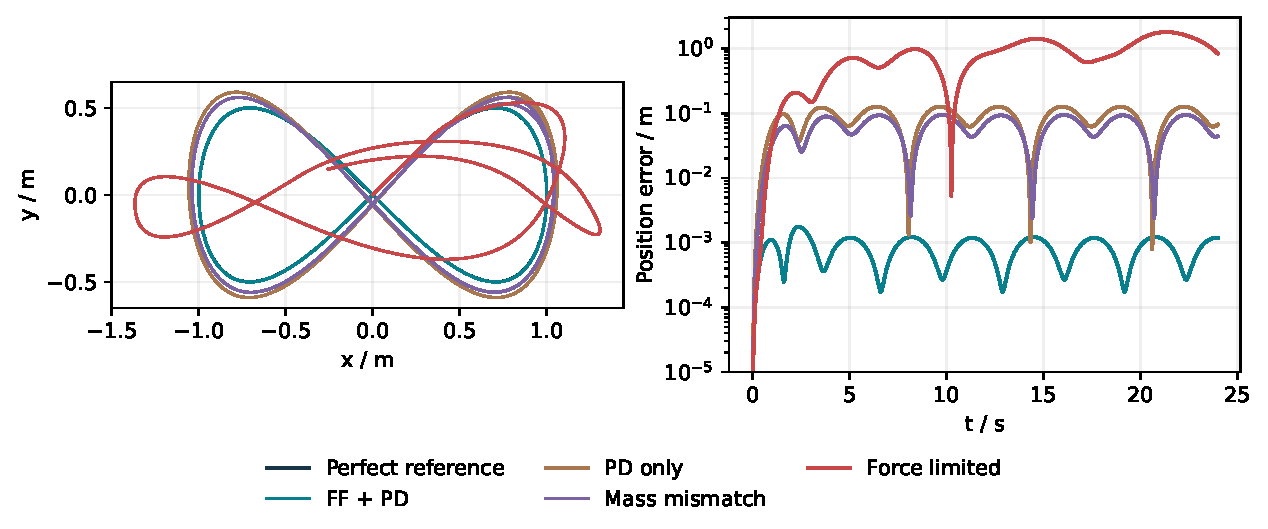
\includegraphics[width=\linewidth]{figures/ch17_pd.pdf}
\caption{八字参考上的几何路线与位置误差。误差纵轴为对数，范围下方的早期值不显示；
理想参考误差为零，不画在对数轴上。每轴 0.2 N 限力导致明显跟踪失败，即使场景仍有足够净空。}
\end{figure}

\begin{center}\small
\begin{tabular}{lrr}\toprule
控制条件 & 圆形 RMS/m & 八字 RMS/m\\\midrule
前馈 + PD，模型匹配 & 0.000393 & 0.000898\\
关闭加速度前馈 & 0.06112 & 0.09151\\
估计质量 0.6 kg & 0.04262 & 0.06691\\
每轴力限 0.2 N & 0.97127 & 0.95082\\\bottomrule
\end{tabular}
\end{center}
关闭前馈仍保留阻力补偿；质量失配组同时将估计转动惯量改为 0.012 kg\,m$^2$。
其他动态组的每轴力限为 2 N、力矩限为 0.2 N\,m。
完整 CSV 还记录最大位置误差、yaw RMS、输入峰值、最小净空和饱和控制次数。
模型匹配的八字实际每轴力峰值约 0.508 N；限力组最大位置误差约 1.802 m。
理想模式直接采样参考，位置误差为零；其力峰值记 NaN，避免误解成“零牛顿也能完成运动”。

\clearpage
\section{参考要平滑起步，不能凭空跳出速度}
直接令相位 $\theta=\omega t$，圆轨迹起点已带速度；本章将相位时钟平滑启动。
给定渐入时长 $R=2$ s，在 $s=t/R\in[0,1]$ 时使用
\begin{equation}
 \tau=R(s^3-\tfrac12s^4),\quad \dot\tau=3s^2-2s^3,\quad
 \ddot\tau=6s(1-s)/R;\qquad \theta=\omega\tau.
\end{equation}
$t\geq R$ 后 $\tau=t-R/2$、$\dot\tau=1$、$\ddot\tau=0$，因此起点静止，连接处 p/v/a 连续。
局部坐标下两种路线分别为
\begin{equation}
 p_{\rm circle}(\theta)=r\begin{bmatrix}\sin\theta\\1-\cos\theta\end{bmatrix},\qquad
 p_{\rm eight}(\theta)=r\begin{bmatrix}\sin\theta\\\tfrac12\sin2\theta\end{bmatrix}.
\end{equation}
用链式法则计算 $v=p_\theta\dot\theta$、$a=p_{\theta\theta}\dot\theta^2+p_\theta\ddot\theta$，
再按参考初始 yaw 旋转到 odom。独立朝向为 $\psi=\psi_0+0.4\sin(\theta/2)$，角速度/角加速度也解析求导。
默认 $r=1$ m、$\omega=0.5$ rad/s；参考尺度与机器人碰撞半径是两件事。

\section{验证、制动与练习}
模型精确、无饱和、理想连续反馈时，可将控制律代入得到
\begin{equation}
 \ddot e_p+K_d\dot e_p+K_pe_p=0.
\end{equation}
此式解释增益作用，却不能直接证明有采样延迟和输入饱和时仍按同样规律收敛。

测试零误差时前馈对应的实际加速度，检查质量和阻力的单位；验证跨 $\pm\pi$ 的 yaw 误差，
检查限幅及阻尼制动力始终反向做功。圆形/八字的 p/v/a 与角导数用中心差分检查，包含渐入连接点。
这些检查验证控制实现的意义，而不只是图看起来贴合。

dampingBrake 按当前速度给出 $F=-\hat m k_bv$、$\tau=-\hat I_zk_b\omega$ 并限幅。
它产生一个新的制动命令，后续 MPC 失败时不会继续发送旧优化结果。
制动需要时间和距离，不代表能在任何障碍前停下，也不自动满足输入变化率限制。

\begin{enumerate}
\item \textbf{推导：}去掉加速度前馈时，误差方程右侧多出什么？模型质量估计偏小时又如何变化？
\item \textbf{代码 ch17-1：}补全逐轴力限幅，解释它和向量范数缩放为什么不同。
\item \textbf{实验：}同样参考依次改变质量估计、阻力和力上限；报告 RMS、最大误差、力峰值与净空，
不能只说“增益更大所以更稳定”。
\end{enumerate}

\chapter{线性 MPC 与约束跟踪}
\begin{notebox}
\textbf{目标}\quad 将受力模型、参考轨迹和线性约束写成 QP；只执行本次有效解的第一步。\\
\textbf{先修}\quad 第 04、13、14、17 章；yaw 仍使用独立前馈 + PD。
\end{notebox}
\section{把连续模型积分成预测矩阵}
\begin{lstlisting}[language=bash]
ros2 run motion2d mpc_demo tmp/ch18_mpc
/usr/bin/python3 scripts/plot_ch18_mpc.py
\end{lstlisting}
取 $x=[p_x,p_y,v_x,v_y]^\top$、$u=[F_x,F_y]^\top$，控制间隔为 $h$。
在一步内保持力不变，令 $\lambda=c_v/m$，$e=e^{-\lambda h}$，
$g=(1-e)/\lambda$，$f=(h-g)/\lambda$，则
\begin{equation}
 x_{k+1}=Ax_k+Bu_k,\qquad
 A=\begin{bmatrix}I&gI\\0&eI\end{bmatrix},\qquad
 B=\begin{bmatrix}(f/m)I\\(g/m)I\end{bmatrix}.
\end{equation}
$\lambda\to0$ 时 $g=h,f=h^2/2$。小阻力应使用第 04 章的稳定极限，避免两个相近数相减。
linearInertialModel 复用精确积分器的基向量响应来提取 A/B；输入取力限内的幅值后归一化。
控制与仿真共用动力学，测试另核对零阻力解析值。

重复代入 N 步，将未来状态和力依次堆叠为 $X=[x_1;\ldots;x_N]$、$U=[u_0;\ldots;u_{N-1}]$：
\begin{equation}
 X=S_xx_0+S_uU,\qquad (S_x)_k=A^k,\qquad
 (S_u)_{k,j}=\begin{cases}A^{k-1-j}B,&0\leq j<k,\\0,&j\geq k.\end{cases}
\end{equation}
预测步数与预测时间不同：$N=20,h=0.02$ s 只看未来 0.4 s。
位置与速度均在 odom，力单位 N。

\section{跟踪、前馈和输入变化组成一个二次型}
未来参考在 $t+h,\ldots,t+Nh$ 采样，前馈力 $U_r$ 由 $\hat m a_r+\hat c_vv_r$ 堆叠。
令 $D$ 为主对角 I、下一条块对角 $-I$ 的差分矩阵，$d=[u_{\rm previous};0;\ldots]$，代价为
\begin{equation}
 J=\|S_xx_0+S_uU-X_r\|_{\bar Q}^2+
 r\|U-U_r\|^2+s\|DU-d\|^2.
\end{equation}
$\bar Q$ 每步对位置与速度分别加权；$r>0$ 使力的二次型正定。
写成 $\tfrac12U^TPU+q^TU+\mathrm{const}$ 后，
\begin{align}
 P&=2(S_u^T\bar Q S_u+rI+sD^TD),\\
 q&=2\{S_u^T\bar Q(S_xx_0-X_r)-rU_r-sD^Td\}.
\end{align}
上一拍必须用\textbf{实际施加的力}，包括制动输入；不能用旧参考或未限幅请求替代。

\clearpage
\section{把约束按行装进矩阵}
求解器的统一形式为 $l\leq C U\leq u$，这里 C 是约束矩阵，避免与动力学 A 混淆。
分别堆叠以下线性行：
\begin{itemize}
\item 力：$-F_{\max}\leq U_i\leq F_{\max}$；两个方向独立。
\item 变化率：$-\dot F_{\max}h\leq DU-d\leq\dot F_{\max}h$，单位 N。
\item 速度：从 $S_xx_0+S_uU$ 取出各步速度，限制两个分量。
\item 走廊：每步选择已验证的配置空间凸区，代入 $H_kp_k\leq b_k$。
\end{itemize}
输入 N 个凸区与 N 个预测状态一一对应；区域已经考虑圆盘半径，不再膨胀一次。
这些约束只限制预测节点，不证明节点之间、定位误差下或跟踪偏离后的连续安全。
ESDF 是非线性距离场，若直接加入非线性约束，就需要另讲 SQP/NMPC，不能继续称作此处的线性 QP。
\lstinputlisting[language=C++,linerange={mpc_condense_begin-mpc_condense_end},includerangemarker=false]{../ros2_ws/src/motion2d/src/control/linear_mpc.cpp}

\section{看得懂的 ADMM 求解器}
本课程独立实现小型稠密正定 QP 求解器，不调用 OSQP 库。
它采用分裂变量 z 将线性系统求解与区间投影分开，主要参考
\href{https://osqp.org/docs/solver/index.html}{OSQP 官方算法说明}，省去稀疏排序、自动缩放和抛光等工程功能。
\lstinputlisting[language=C++,linerange={qp_admm_begin-qp_admm_end},includerangemarker=false]{../ros2_ws/src/motion2d/src/optimization/box_qp.cpp}
这里 solve 使用缓存的 LDLT 分解；每 25 次迭代按归一化残差调整 $\rho$，变化足够大时重新分解。
只有原始残差 $CU-z$ 与对偶残差 $PU+q+C^Ty$ 均满足绝对/相对容差才返回 solved。
默认容差均为 $10^{-5}$、最多 1500 次；无约束测试对照解析解 $-P^{-1}q$。

\clearpage
\section{失败状态与短时域的边界}
成功后仅施加 $u_0$；下一次重读状态、重建 QP。
上次成功 U 左移一块、重复尾块，作为本次初值；失败立即清空热启动并生成新的限幅阻尼力。
稠密构建、分解和迭代适合本章小问题，不承诺硬实时。
\begin{center}\small
\begin{tabular}{lp{9cm}}\toprule
状态 & 可得结论\\\midrule
solved & 残差在设定容差内；不是连续碰撞或闭环稳定性证明\\
primal\_infeasible & 上下界矛盾，或找到近似归一化不可行证书\\
max\_iterations & 给定迭代数内没收敛；不能因此断言问题不可行\\
time\_limit & 迭代间检查到墙钟预算用完；当前迭代可超出预算\\
numerical\_failure & 非有限迭代；不能继续使用该输入序列\\\bottomrule
\end{tabular}
\end{center}
不可行证书满足 $C^Tv\approx0$ 且 $u^Tv_++l^Tv_-<0$；非有限单侧边界不能参与错误的有限乘积。
无效外部维度或非正定代价直接报错；示例对超时和迭代不足分别验收。
制动仍只保证力限幅，\textbf{不保证输入变化率、停止路径或失去观测后的速度准确性}。

\paragraph{一个可复现的不可行例子}
测试用 1 kg、阻力 0.15、力限 0.8 N、变化率 0.8 N/s，$h=0.1$ s、$N=12$，
走廊右边界 $x=0.3$ m，却让代价追逐 $x_r=1$ m。
前几次 QP 都满足各自节点约束，第八次则不可行。
独立检查每一步所能用的最小 x 力 $\max(-F_{\max},u_{\rm previous}-j\dot F_{\max}h)$，
即使这样尽早减力，第 12 步仍到约 0.30618 m，超过边界。
有限时域末端还带着速度，下一次多看到一步时便发现来不及停。
终端安全集合、可停车参考和约束收紧是进一步方法；本章不宣称已实现递归可行性保证。

\paragraph{练习与独立检查}
\begin{enumerate}
\item 推导一步 A/B 的零阻力极限，并核对 kg、N、m/s 的单位。
\item \textbf{ch18-1：}补全输入差分矩阵；解释为什么首块要减上一拍实际输入。
\item 显式滚动积分并计算各项代价，用中心差分核对凝聚后梯度 $PU+q$。
\item 固定参考比较 PD/MPC、预测长度和控制频率；记录失败次数、实际变化率与求解耗时，不能只画误差。
\end{enumerate}

\clearpage
\section{同一八字参考上的实测对照}
使用第 17 章相同八字、24 s、200 Hz 物理积分、1 kg 与 0.15 kg/s 阻力，
初始静止，yaw 使用相同 PD；本表没有通信延迟或估计噪声。
MPC 默认位置/速度权重 40/2、力权重 0.02、增量权重 0.005；不加终端集合。
2 N 组速度分量限 1 m/s、力变化率限 5 N/s。

\begin{center}\small
\begin{tabular}{lrrrr}\toprule
方法 & N & 控制/Hz & 位置 RMS/m & 耗时 P95/ms\\\midrule
前馈 + PD & -- & 50 & $8.98\times10^{-4}$ & --\\
MPC & 10 & 50 & $4.63\times10^{-5}$ & 0.0300\\
MPC & 20 & 50 & $9.37\times10^{-6}$ & 0.0826\\
MPC & 40 & 50 & $5.56\times10^{-6}$ & 0.4114\\
MPC & 20 & 20 & $1.44\times10^{-5}$ & 0.0790\\\bottomrule
\end{tabular}
\end{center}
所有常规组均无求解失败。耗时包含 QP 组装、分解、迭代和热启动更新，不含 ROS 或绘图；
主机 Ryzen 7 9700X、GCC 15.2、RelWithDebInfo，未锁频或绑核。
较长时域在此例更精确也更慢；20 Hz 组 $Nh=1$ s，与 50 Hz 的 0.4 s 不是同一个前瞻时间。
极小误差来自准确模型与未来参考，不能照搬为真实传感器系统的性能。

\begin{figure}[!ht]
\centering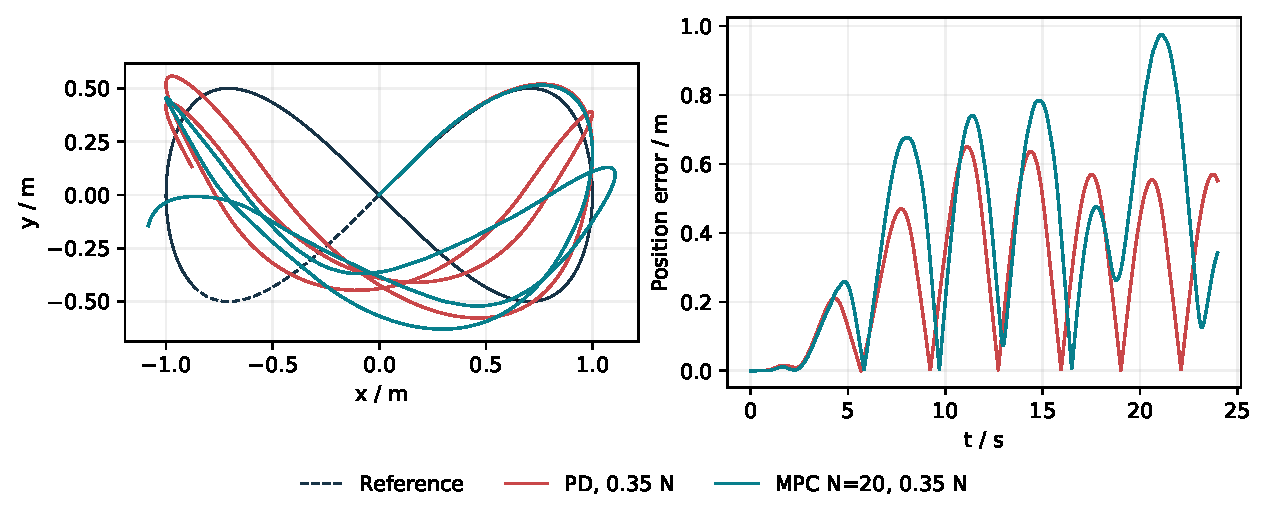
\includegraphics[width=\linewidth]{figures/ch18_mpc.pdf}
\caption{将力限收紧到每轴 0.35 N。两种方法都无法紧贴原参考；MPC 还施加每轴 0.5 m/s 和 2 N/s 约束。
它的失败会切换到制动，因此不能把整条实际输入曲线都称为满足 QP 约束。}
\end{figure}

限力 PD 的 RMS 为 0.3533 m，MPC 为 0.4771 m；MPC 并非所有参数下都更好。
PD 最大速度分量 0.5992 m/s；MPC 约 0.500001 m/s，后者的微小超量在数值容差量级。
MPC 有 21 次 max\_iterations，不能据此断言不可行；制动切换导致实际最大力变化率达 35 N/s。
其最小净空仍有 2.6933 m，但空房间的这次结果不证明任意障碍场景安全。
完整 summary.csv 与 failures.csv 分开记录各次误差、耗时、状态及新的制动力。

\chapter{接通在线规划与完整导航}
\begin{notebox}
\textbf{目标}\quad 将定位、地图、局部规划和跟踪连成闭环；理解未来参考接续、坐标冻结与导航误差的计算。\\
\textbf{先修}\quad 第 08--18 章。先运行参考交接例子，再启动完整导航，最后比较不同机器人模型。
\end{notebox}
\section{运动带来新观测，新观测改变下一次计划}
前几章分别建立了传感器、估计器、地图、轨迹和控制器。
导航把它们连接起来：机器人向前走，看见原来被遮挡的区域；新地图又改变接下来可走的路线。
规划因此需要反复更新，而控制器在计算新计划期间仍要持续跟踪已有参考。

\begin{center}\begin{minipage}{\linewidth}\makeatletter\def\@captype{figure}\makeatother
\centering
\begin{tikzpicture}[>=Stealth,node distance=.55cm,
 b/.style={draw=tealblue,fill=pale,rounded corners,minimum width=2.05cm,minimum height=.85cm,align=center,font=\small}]
\node[b] (s) {激光与 IMU};\node[b,right=of s] (m) {定位与地图};
\node[b,right=of m] (p) {局部规划};\node[b,right=of p] (c) {跟踪控制};\node[b,right=of c] (r) {机器人};
\draw[->] (s)--(m);\draw[->] (m)--(p);\draw[->] (p)--(c);\draw[->] (c)--(r);
\draw[->] (r.south)--++(0,-.8)-| (s.south);
\node[fill=white,font=\small] at(5.2,-.8) {运动改变下一帧观测};
\node[above=.5cm of p,font=\small] (g) {地图中的目标};\draw[->] (g)--(p);
\end{tikzpicture}
\caption{导航的闭环关系。定位产生的当前状态同时供规划和控制使用；地图描述机器人已经观测到的空间。}
\end{minipage}\end{center}
每个模块使用不同的时间尺度：IMU 与动力学更新较快，激光和地图较慢，优化还需要计算时间。
本章先解决参考如何在未来时刻平滑交接，再解释规划时使用哪一份地图，以及控制器如何接收这个计划。

\section{新曲线从未来交接状态出发}
\begin{lstlisting}[language=bash,numbers=none]
ros2 run motion2d reference_handover_demo tmp/ch19_handover
/usr/bin/python3 scripts/plot_ch19_handover.py
\end{lstlisting}
设现在的绝对仿真时间为 $t_0$，预留 $\Delta>0$ 的计算和传输时间，计划在 $t_s=t_0+\Delta$ 交接。
旧曲线的绝对起点为 $t_b$，因此它在交接处的局部时间是 $\tau_s=t_s-t_b$。
新曲线的局部时间则从零开始，首边界应设为
\begin{equation}
 p_n(0)=p_o(\tau_s),\qquad v_n(0)=v_o(\tau_s),\qquad a_n(0)=a_o(\tau_s).\label{eq:handover}
\end{equation}
整体参考为 $p(t)=p_o(t-t_b)$（$t<t_s$）和 $p(t)=p_n(t-t_s)$（$t\geq t_s$）。
从左右分别取极限，式\eqref{eq:handover}使位置及其一、二阶导数都相等，这就是 $C^2$ 接续。
由 $F=ma+c_vv$，模型匹配时的平移前馈力也连续。
jerk 是加速度的导数；当前边界没有匹配它，因此力的变化率可能在交接处改变。

\subsection{在旧曲线上手算首边界}
示例旧曲线从 $(0,0)$ 静止走到 $(2,0)$，时长 4 s。
用第 14 章的 $h(s)=10s^3-15s^4+6s^5$，有 $p_x=2h(t/4)$。
在绝对起点为零、$t_s=1.5$ s 时，$s=3/8$，逐项求导得到
\[
 p_x=2h(3/8)=0.550415\text{ m},\quad
 v_x=\tfrac24h'(3/8)=0.823975\text{ m/s},\quad
 a_x=\tfrac2{16}h''(3/8)=0.439453\text{ m/s}^2.
\]
新曲线从这组边界出发，用 4 s 转向 $(3,1)$ 并停下。
如果只匹配位置而把新速度设成零，参考速度会跳变约 0.824 m/s；在 0.02 s 的控制间隔上，
对应约 41.2 m/s$^2$ 的速度变化要求。保留旧参考的导数能避免这种人为突变。
\begin{center}\begin{minipage}{\linewidth}\makeatletter\def\@captype{figure}\makeatother
\centering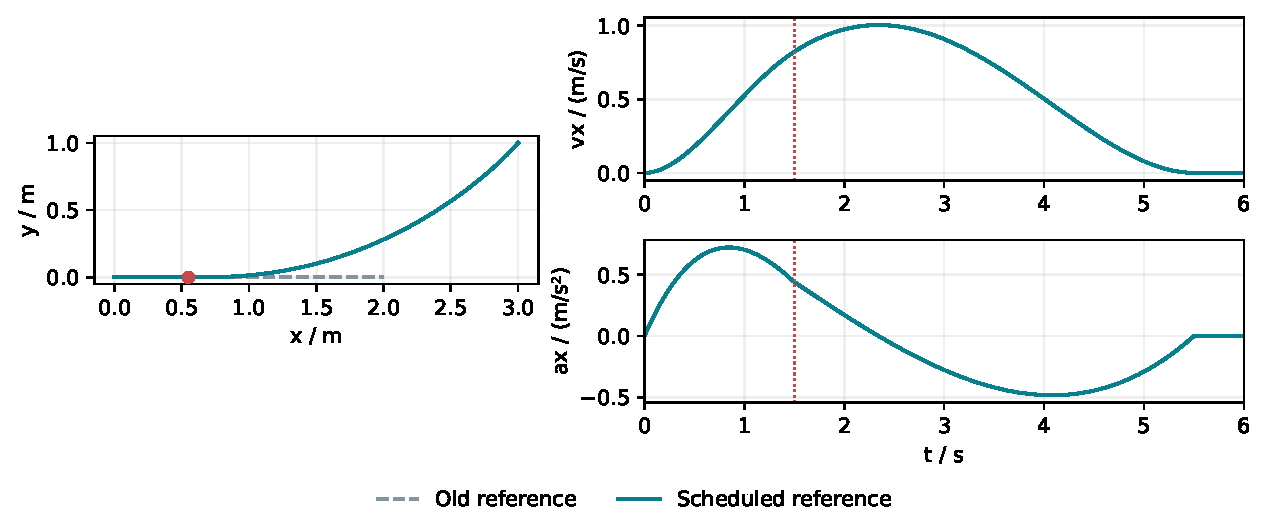
\includegraphics[width=\linewidth]{figures/ch19_handover.pdf}
\caption{在 1.5 s 交接。旧曲线原本沿 x 轴到达 (2,0)，新曲线转向 (3,1)；
红点和竖虚线标记交接时刻。速度与加速度保持连续，jerk 不要求连续。}
\end{minipage}\end{center}
规划计算期间继续执行旧曲线，反馈处理实际状态相对旧参考的偏差。
如果偏差已使现有走廊余量不足，则先制动、重新静止定位，再建立下一条参考。
这一操作与平滑接续分别对应两种控制状态，应在状态记录和误差曲线上标出。

\section{查询未来与推进当前是两件操作}
MPC 在时刻 $t_0$ 就会查询 $t_0+h,\ldots,t_0+Nh$，其中可能有时刻已经越过 $t_s$。
调度器需要按查询时间返回正确曲线，同时保留真正的当前活动曲线。
\code{ReferenceSchedule} 保存 \code{active} 与至多一条 \code{pending}，其行为可按时间表理解：
\begin{center}\small
\begin{tabular}{lll}\toprule
实际观测时刻 & 查询时刻 & 应返回的参考\\\midrule
1.2 s & 1.3 s & 旧曲线\\
1.2 s & 1.6 s & 未来候选，但保留旧活动曲线\\
1.2 s & 1.2 s & 仍为旧曲线\\
1.5 s & 1.6 s & 已交接的新活动曲线\\\bottomrule
\end{tabular}
\end{center}
\code{sample} 是只读查询，\code{advance} 由实际推进的观测时刻调用，达到 $t_s$ 才把候选变成活动曲线。
接收新曲线时，先用同一绝对起点查询旧参考，再检查首边界：
\par\noindent\begin{minipage}{\linewidth}
\lstinputlisting[language=C++,linerange={reference_handover_begin-reference_handover_end},includerangemarker=false]{../ros2_ws/src/motion2d/src/trajectory/reference_schedule.cpp}
\end{minipage}\par
三个范数分别比较位置、速度和加速度，最后还匹配固定 yaw。
$10^{-7}$ 用于数值计算后的同一边界比较；每项保持自己的 SI 单位。
终点 v/a 必须为零，这样到达以后可接上恒定位置保持。
起点已经过去、第二条候选仍待交接或边界不匹配时，保留原有效计划并返回原因；
显式 \code{reset} 则清空两条参考，把静止锚点设为新的位姿。

\section{规划时冻结 map 与 odom 的变换}
回环校正改变地图与局部里程计之间的对齐。设本次规划采用
\[
 p_m=Rp_o+b,
\]
其中 $R,b$ 在本次求解和参考转换中保持固定。由 $R^TR=I$，反解并对时间求导：
\begin{equation}
 p_o=R^T(p_m-b),\qquad v_o=R^Tv_m,\qquad a_o=R^Ta_m.\label{eq:navframe}
\end{equation}
位置含平移，导数中的常量平移消失。
将 $p_m(t)=\sum_{k=0}^5c_{m,k}t^k$ 代入，逐次幂收集，得到
\[
 c_{o,0}=R^T(c_{m,0}-b),\qquad c_{o,k}=R^Tc_{m,k}\quad(k\geq1).
\]
走廊顶点也使用同一变换，再重新构造半空间；固定 yaw 减去 $R$ 对应的旋转角。

例如 $R$ 表示 $90^\circ$ 旋转、$b=(1,2)$，地图位置 $(1,3)$、速度 $(0,0.5)$
转换为 odom 位置 $(1,0)$、速度 $(0.5,0)$。
若下一次地图平移校正为 $(1.1,2)$，把旧地图系数直接重新转换会让其 odom 位置跳到 $(1,0.1)$。
因此已发送的 odom 系数保持固定；新的变换用于下一次规划，并从旧 odom 参考的未来边界接续。

\code{transformReference} 对曲线与各区域统一转换。
新地图到达后，还要把剩余 odom 区域按当前对齐放回 map，检查它们是否仍在新的自由配置空间中。
这样既保留控制参考的连续性，也及时响应新发现的障碍。

\section{在已观测空间中选一个可达的局部目标}
\begin{lstlisting}[language=bash,numbers=none]
ros2 run motion2d replanner_demo tmp/ch19_replanner
/usr/bin/python3 scripts/plot_ch19_replanner.py
\end{lstlisting}
一次规划读取同一时刻的地图快照：原始占据栅格、由它膨胀的配置空间栅格、同源未膨胀 ESDF。
原始栅格回答哪里未知、哪里有障碍；膨胀栅格回答圆心可经过哪里；ESDF 给出优化所用的距离与梯度。
这些数据来自同一份地图，才能让路径搜索和曲线检查使用一致的几何。

从未来交接点所在自由格做八邻接可达搜索，斜向连接按第 11 章禁止切角。
如果全局目标已可达，直接用 A* 搜索它；否则在可达自由格中选择邻近未知区的\textbf{前沿候选}。
因为未知区周围已经膨胀，候选不一定紧挨原始未知格。代码检查的窗口半径为
\[
 n_w=\left\lceil\frac{r_{\rm clearance}}{d}\right\rceil+2,
\]
$d$ 为分辨率。除以 $d$ 把米换成格数，向上取整覆盖膨胀距离，额外两格容纳格子边界与搜索邻域。
例如 $r_{\rm clearance}=0.15$ m、$d=0.1$ m，得到四格窗口。

对候选中心 $q$ 比较 $\|q-g\|^2$，选离全局目标 $g$ 最近者。
平方距离与距离的大小顺序相同，省去了逐候选开方。
还要求 $\|p_s-g\|-\|q-g\|\geq0.1$ m，避免在几乎不前进的候选间反复切换。
在需要先远离目标才能绕出的凹形环境中，这一规则可能停滞；可进一步加入访问历史或信息增益来改进探索。

\begin{center}\small
\begin{tabular}{lp{8.5cm}}\toprule
局部搜索状态 & 可以据此检查什么\\\midrule
no\_reachable\_frontier & 已可达自由区内没有邻近未知区的候选；查看遮挡和地图边界\\
no\_progress\_frontier & 候选离目标的改善小于阈值；查看是否需要先绕远\\
goal\_occupied / goal\_outside\_map & 目标在当前占据格或地图范围之外；重新选目标\\\bottomrule
\end{tabular}
\end{center}
搜索得到折线后，沿长度截取局部前缀，默认最多 2 m。
若已累计长度 $L$，下一段向量为 $d_p$，而剩余长度 $\ell_{\max}-L<\|d_p\|$，截断点是
\[
 q_{\rm cut}=q_{\rm last}+\frac{\ell_{\max}-L}{\|d_p\|}d_p.
\]
比例位于 $[0,1]$，所以新点仍在已经检查过的自由线段上。
例如剩 0.5 m、下一段为 $(0.6,0.8)$ m，其长度为 1 m，只走 $(0.3,0.4)$ m。
\begin{center}\begin{minipage}{\linewidth}\makeatletter\def\@captype{figure}\makeatother
\centering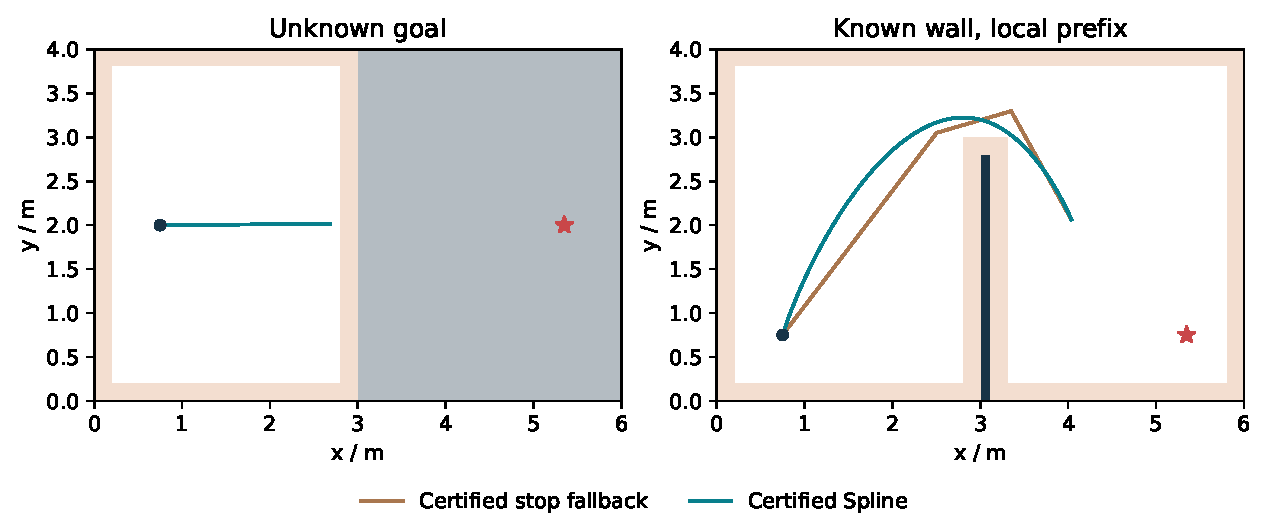
\includegraphics[width=\linewidth]{figures/ch19_replanner.pdf}
\caption{两张用于学习局部目标选择的占据网格。灰色未知、深蓝占据、浅橙为配置空间阻塞；
星号是全局目标，曲线只到达当前局部终点。左图不穿越未知区，右图采用最多 5 m 的路线前缀绕墙。}
\end{minipage}\end{center}
图中网格为 $60\times40$、分辨率 0.1 m，机器人半径 0.1 m、额外余量 0.05 m。
左侧只有 $x<3$ m 已观测，局部目标逐渐靠近未知边缘；右侧全图已知，演示最多 5 m 的绕墙路线前缀。
新的扫描扩展自由空间后，再用新快照选择下一段目标。

\section{从未来边界生成并检查局部曲线}
对局部路线构建凸走廊，起点使用式\eqref{eq:handover}的未来 p/v/a，终点设为静止。
Spline 优化使用第 15、16 章的能量、ESDF、走廊及导数代价。
核心演示默认控制点走廊权重 50000、额外内缩 0.04 m，软速度/加速度目标 0.45/0.5，
最终连续上界要求速度 0.7 m/s、加速度 0.8 m/s$^2$。
软目标帮助求解靠近可行区域，Bézier 连续界再逐段检查最终曲线。

优化结果未通过时，备用方案在各路点停下，\textbf{首段仍保留旧参考的 p/v/a}。
依次尝试基准时长及其 1.5、2、3 倍，并对每条候选作同样的连续检查。
\par\noindent\begin{minipage}{\linewidth}
\lstinputlisting[language=C++,linerange={replanner_fallback_begin-replanner_fallback_end},includerangemarker=false]{../ros2_ws/src/motion2d/src/planning/replanner.cpp}
\end{minipage}\par
\code{left=start} 保留移动起点；\code{right} 的导数默认零。
只有第一段之后，左边界才变成刚构造的静止右边界。
\code{certifyBezier} 检查同一组区域和导数限制，成功时才返回候选。

\subsection{为什么延长时长有时会把曲线推出走廊}
静止到静止时，同一形状可以通过延长时间降低导数。
但首速度 $v_0$ 已经固定时，曲线形状也随时长变化。用单轴起点位置零、首加速度零、终点位置 $D$ 且静止的五次段说明。
由第 14 章端点公式，令 $s=t/T$，可整理为
\[
 p(t)=D h(s)+v_0T b(s),\quad
 b(s)=s-6s^3+8s^4-3s^5.
\]
$h$ 提供静止到静止的位移；$b(0)=b(1)=0,b'(0)=1,b'(1)=0,b''(0)=b''(1)=0$，
因此第二项恰好补上首速度 $v_0$，其余边界保持不变。
在中点 $h(1/2)=1/2,b(1/2)=5/32$，所以
\[
 p(T/2)=D/2+5v_0T/32.
\]
取 $D=1$ m、$v_0=0.5$ m/s，$T=2$ s 时中点为 0.65625 m，$T=8$ s 时却到 1.125 m。
较长时间让初始速度带来更大的前冲。备用时长每改一次，都要重新检查空间与动力学界。

局部例子的总时长如下，优化目标包含平滑性与软约束，因此时间会随整个目标的权衡变化。
\begin{center}\small
\begin{tabular}{lrr}\toprule
场景 & 逐段停车/s & Spline/s\\\midrule
未知目标的局部前缀 & 7.258 & 11.424\\
绕墙的 5 m 前缀 & 19.466 & 12.994\\\bottomrule
\end{tabular}\end{center}
这组演示关闭优化墙钟预算以便观察解的差别；在线节点另设计算预算。
返回状态区分 \code{optimized} 与 \code{fallback_stop_segments}，并保存优化器原始状态。
所有候选都未通过时，上层进入制动与静止重试。

\section{把曲线与走廊一起交给控制器}
一条执行参考需要同时说明曲线、绝对起点、对应区域和地图快照时刻。
\code{NavigationReference} 将这些内容放在同一消息中，让控制器收到的是一套配对数据。
否则两条独立话题的到达次序可能把新曲线与旧走廊配在一起。
区域顶点采用 float64，与曲线计算保持相同精度。

接收器先检查坐标、分段与区域数量，再检查曲线在区域中的连续界，以及未来交接的 p/v/a/yaw。
接收成功后发布携带绝对起点纳秒的确认。
规划端收到匹配的确认，才将候选放进自己的参考调度，从而与控制端保持一致。

\begin{center}\begin{minipage}{\linewidth}\makeatletter\def\@captype{figure}\makeatother
\centering\begin{tikzpicture}[x=1cm,y=1cm,>=Stealth]
\node at(0,0) {规划端};\node at(7,0) {控制端};
\draw[->,muted] (0,-.3)--(0,-3.2);\draw[->,muted] (7,-.3)--(7,-3.2);
\draw[->,tealblue,thick] (0,-.7)--(7,-1.2) node[midway,above,sloped,font=\small] {曲线、区域、未来起点 $t_s$};
\node[right,font=\small] at(7,-1.5) {检查边界与连续界};
\draw[->,navy] (7,-1.9)--(0,-2.3) node[midway,above,sloped,font=\small] {确认同一个 $t_s$};
\draw[dashed,muted] (-.5,-2.8)--(7.5,-2.8);
\node[left,font=\small] at(-.5,-2.8) {$t_s$};
\node[right,font=\small] at(7,-2.8) {开始执行};
\end{tikzpicture}
\caption{确认与开始执行分开。候选在未来起点之前通过接收检查；确认携带该起点，规划端据此匹配自己的待确认计划。}
\end{minipage}\end{center}

\begin{center}\small
\begin{tabular}{ll}\toprule
话题 & 语义\\\midrule
/navigation/reference & odom 系完整候选\\
/control/accepted\_reference & 已接收候选的起点纳秒\\
/navigation/stop & 清空参考并切换制动\\
/control/reference & 当前观测时刻的参考位姿、机体系速度\\
/control/reference\_acceleration & 同时刻的 odom 加速度\\\bottomrule
\end{tabular}\end{center}
MPC 查询未来参考时，也查询该时刻对应的区域；首条曲线尚未开始时，静止保持使用第一个区域。
等待确认或等待交接时暂缓第二条候选，确保各自保存的状态简单一致。

\subsection{首次启动与移动接续的不同边界}
首次启动和制动后重新启动时，观测速度、角速度分别小于 0.02 m/s、0.02 rad/s，
首点距当前位置不超过 0.03 m，yaw 差不超过 0.02 rad，并要求首 v/a 为零。
这组小容差接纳静止测量波动。已有活动参考时，则直接匹配未来旧边界，使用前面的数值精度容差。

可先用合成时钟实验跟踪一次接收过程：
\begin{lstlisting}[language=bash,numbers=none]
ros2 run motion2d tracker_node --ros-args \
  -p use_sim_time:=true -p reference.source:=navigation \
  -p control.odometry_timeout:=10.0
# Another terminal; this script supplies /clock and observations.
python3 scripts/check_navigation_boundary.py
\end{lstlisting}
示例先沿 x 轴运动，再在 0.7 s 接续转向。删除候选的一个区域后，接收器返回数量错误，旧曲线继续使用。
显式停车则清空计划并按当前速度制动；停车过程使用第 17 章的动力学，下一次起步重新建立静止锚点。

\section{观测驱动的导航节点}
\begin{lstlisting}[language=bash,numbers=none]
ros2 launch motion2d_bringup ch19.launch.py route:=B
ros2 service call /sim/pause std_srvs/srv/SetBool '{data: false}'
ros2 topic pub --once /goal_pose geometry_msgs/msg/PoseStamped \
  '{header: {frame_id: map}, pose: {
     position: {x: -4.0, y: -4.0}, orientation: {w: 1.0}}}'
\end{lstlisting}
也可在 RViz 使用 2D Goal Pose。地图回调生成原始/膨胀/ESDF 快照，里程计回调推进参考调度，
扫描时间戳用于判断传感器是否持续更新。默认规划频率 5 Hz，MPC 控制 50 Hz；理想点模式按 200 Hz 发下一仿真步的位置。

设上次尝试时刻为 $t_l$、周期为 $P$，满足 $t-t_l\geq P$ 且没有待交接候选时才开始新规划。
例如 $P=0.2$ s、$t_l=1.0$ s，在 1.19 s 等待，1.20 s 触发。
判断使用仿真时间，所以暂停时墙钟计时器唤醒也不会反复规划。
时钟回退意味着开始新的仿真过程，节点清空目标与旧快照，再等待新目标。

每次预留 0.15 s 作为交接提前量，优化墙钟预算为 0.04 s。
路径搜索、区域构建和传输也占用时间，故确认必须在起点之前到达。
核心代码先把未来旧边界变到 map，在同一快照上规划，再将结果和区域一起变回 odom：
\par\noindent\begin{minipage}{\linewidth}
\lstinputlisting[language=C++,linerange={navigation_snapshot_begin-navigation_snapshot_end},includerangemarker=false]{../ros2_ws/src/motion2d/src/nodes/navigation_node.cpp}
\end{minipage}\par
\code{old} 来自未来参考查询，\code{boundary} 是 map 系的首 p/v/a。
\code{awaiting_} 保存已发出、等待确认的候选；确认回调再更新本地调度。
TF 使用最近可用的 map/odom 对齐并在本次求解期间固定，适应 IMU 更新快于 SLAM 对齐的情况。

新地图到达后检查所有尚未执行完的区域，包括待确认候选。
扫描年龄超过 0.35 s、里程计超过 0.12 s 或地图超过 3 s 时，参考清空并制动。
规划候选未通过、确认超时或 MPC 未成功求解时，也转入这一流程。
保留的目标在静止后重试。若多次停在同一区域，应结合前沿状态、地图和激光覆盖，判断是缺少观测还是路线不可执行。

\section{同场景逐步接入惯性与估计误差}
三条路线逐层增加复杂度：
\begin{center}\small
\begin{tabular}{llll}\toprule
路线 & 定位 & 地图 & 控制\\\midrule
A & 真值适配器 & 扫描观测建图 & 理想点设定\\
B & 真值适配器 & 扫描观测建图 & 惯性模型 + MPC\\
C & 激光/IMU、EKF、关键帧 SLAM & 关键帧观测地图 & 惯性模型 + MPC\\\bottomrule
\end{tabular}\end{center}
A 到 B 观察动力学和跟踪的影响，B 到 C 再观察估计误差的影响。
完整障碍列表与真值位姿由独立评价器读取；导航所用自由空间均来自传感器观测。
C 的 map/odom 对齐由 SLAM 发布。
\begin{lstlisting}[language=bash,numbers=none]
# The script launches each trial in its own ROS domain.
python3 scripts/run_ch19.py --seeds 42 43 44
python3 scripts/plot_ch19_navigation.py
\end{lstlisting}
世界为 $20\times20$ m，含 8 个圆和 8 个凸多边形，圆盘半径 0.2 m。
同一随机种子对应同一几何。激光为 720 束、10 Hz、6 m 量程，每束标准差 0.01 m；
B/C 使用 200 Hz IMU，白噪声沿用第 06 章，动力学阻尼与第 18 章相同。
地图分辨率 0.1 m，配置空间额外留 0.15 m 跟踪余量。
在线节点采用轨迹采样软惩罚，再用独立 Bézier 连续界检查执行候选。

物理起点为 $(-8,-8)$，目标为 $(-4,-4)$，初始 yaw 为零。
A/B 中 map 与 world 相同；C 的第一帧设为 map 原点，同一物理目标因此约为 $(4,4)$。
例如无旋转时，$p_m=p_w-(-8,-8)$，直接代入即可得到这一差别。
当前 C 配置以初始 yaw 为零对齐估计 odom 与物理施力轴；扩展初始朝向时，要同时旋转力向量接口。
到达判据为选定定位距目标小于 0.12 m 且速度小于 0.08 m/s，评价器还检查真实目标误差小于 0.25 m。
\begin{center}\begin{minipage}{\linewidth}\makeatletter\def\@captype{figure}\makeatother
\centering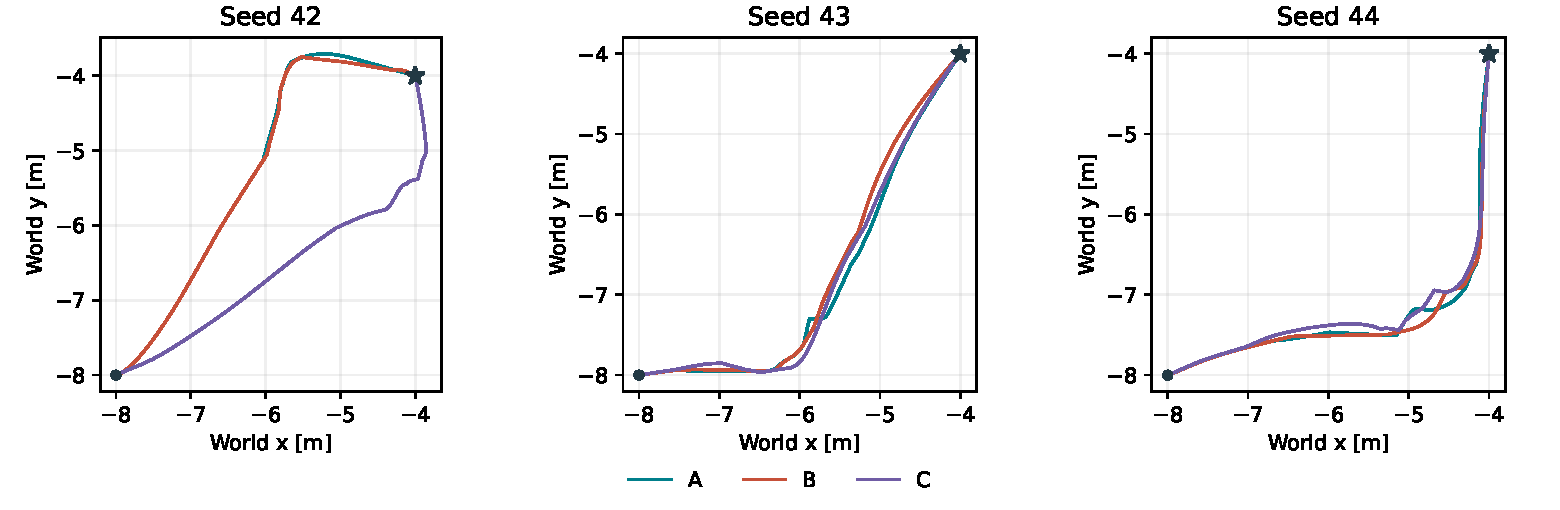
\includegraphics[width=\linewidth]{figures/ch19_navigation.pdf}
\caption{三个随机世界中的圆心轨迹，统一画在 world 坐标中，圆点为起点、星号为目标。
三种路线使用同一世界和目标，障碍净空由完整几何计算。}
\end{minipage}\end{center}
\section{分别计算定位误差、短时漂移与跟踪误差}
\subsection{先把估计位姿放进同一个世界坐标系}
用第 02 章的位姿变换记号 $T=(R,p)$，其作用是 $q\mapsto Rq+p$。
记真实位姿为 $T_i^w$，估计 odom 位姿为 $O_i$，该时刻最近可用的 map/odom 对齐为 $M_i$，
则地图中的估计位姿为 $\widehat T_i=M_iO_i$。
地图原点可以任意选择，先用第一帧确定一个固定对齐
\[
 G=T_0^w(\widehat T_0)^{-1},\qquad \widetilde T_i=G\widehat T_i.
\]
代入 $i=0$ 可见 $\widetilde T_0=T_0^w$，之后对齐 $G$ 保持不变。
这样消除的是初始坐标选择，后续累积的定位误差仍会反映在比较中。

\textbf{绝对轨迹误差}（ATE）在本章取平移部分：
\[
 e_i^{\rm ATE}=\operatorname{pos}(\widetilde T_i)-\operatorname{pos}(T_i^w),\qquad
 \mathrm{ATE}_{\rm RMS}=\sqrt{\frac1N\sum_i\|e_i^{\rm ATE}\|^2}.
\]
\code{pos} 表示取位姿中的位置向量。平方消去误差方向的正负，平均反映整段轨迹，开方后单位恢复为米。
例如两个位置误差为 $(0.01,0)$ 和 $(0,0.02)$ m，RMS 为 $\sqrt{(0.01^2+0.02^2)/2}\approx0.01581$ m。

\subsection{用相对运动检查一秒内积累的误差}
\textbf{相对位姿误差}（RPE）先比较两帧之间的运动。
真实与估计的相对变换分别为
\[
 D_{ij}=(T_i^w)^{-1}T_j^w,\qquad\widehat D_{ij}=O_i^{-1}O_j,\qquad
 E_{ij}=D_{ij}^{-1}\widehat D_{ij}.
\]
若两种运动相同，$E_{ij}$ 为单位变换。
展开第 02 章的逆变换和复合式，真实相对平移是
$R_i^T(p_j-p_i)$，表示“从第 $i$ 帧车身看，第 $j$ 帧移动到哪里”。
估计相对平移同样计算；再求两种相对变换之间的误差。
本章选择 $t_j-t_i=1$ s，取 $\|\operatorname{pos}(E_{ij})\|$ 的 RMS。
实现使用\textbf{连续 odom 位姿}计算 RPE，用带地图校正的位姿计算 ATE，分别观察短时运动与整体定位。

例如方向均为零，真值一秒前进 1 m、估计前进 1.02 m，平移 RPE 为 0.02 m。
给所有估计位姿左乘同一个固定变换 $H$，相对运动仍是
$(HO_i)^{-1}(HO_j)=O_i^{-1}O_j$，所以 RPE 对固定坐标原点的选择不敏感。

\subsection{跟踪误差与物理净空}
跟踪误差比较相同时间戳、同一 odom 系的观测位置与控制参考：
\[
 e_i^{\rm track}=p_i^{\rm odom}-p_{r,i}^{\rm odom}.
\]
它回答控制器是否跟上了自己使用的参考。
在已经对齐的一维例子中，某时刻估计位置与参考都为 1.1 m、真实位置为 1.0 m，跟踪误差为零，而估计相对真值仍偏了 0.1 m。
因此要分别查看定位和跟踪曲线。
\code{check_ch19.py} 按精确时间戳配对样本；RPE 只使用能找到一秒后对应样本的时刻。

真实圆盘净空为 $d_{\rm true}(p)-r$，其中 $d_{\rm true}$ 是真值圆心到完整障碍边界的最短距离，
计算方法见第 03 章。它检查实际外形离障碍还有多远；规划 ESDF 则描述当前观测地图中的距离。
评价还记录到达时间、停车次数、规划与控制耗时，这些量一起描述导航过程。

\section{读懂三条路线的对照结果}
\begin{center}\small
\begin{tabular}{lrrrrr}\toprule
路线/种子 & 到达/s & ATE/mm & 跟踪/mm & 净空/m & 停车\\\midrule
A/42 & 20.80 & 0.00 & 0.00 & 0.444 & 10\\
B/42 & 24.05 & 0.00 & 0.41 & 0.406 & 6\\
C/42 & 26.44 & 5.40 & 2.02 & 0.370 & 6\\
A/43 & 26.18 & 0.00 & 0.00 & 0.481 & 13\\
B/43 & 24.02 & 0.00 & 0.46 & 0.474 & 6\\
C/43 & 24.91 & 4.95 & 2.04 & 0.417 & 6\\
A/44 & 24.52 & 0.00 & 0.00 & 0.530 & 7\\
B/44 & 27.61 & 0.00 & 0.38 & 0.574 & 7\\
C/44 & 28.23 & 5.76 & 1.76 & 0.435 & 7\\
\bottomrule\end{tabular}
\end{center}
表中 ATE 和跟踪均为 RMS，净空为全程最小真实圆盘净空。
A/B 采用真值定位，零 ATE 是该输入模式的定义；A 的理想点设定用于建立几何基线。
C 的三次一秒平移 RPE 为 2.57、2.21、2.55 mm。
B/C 的 MPC 在这组运行中均完成求解；停车主要发生在新地图使旧区域失效或局部候选未通过时。
查看停车前后的状态，可以理解参考接续与重新静止起步如何配合。

这九组在三个固定随机世界中均到达目标，碰撞尝试为零。
规划 P95 耗时为 6.96--10.13 ms，B/C 的 MPC P95 为 0.38--0.46 ms。
规划计时包括局部路线、走廊和轨迹求解；地图回调中的膨胀与 ESDF、消息传输和显示另行耗时。
换用更长路线或更密集障碍时，应重新记录这些阶段的时间分布。

初始未知格约占 88.9\%--92.9\%，到达时仍有约 74.7\%--76.4\% 未知。
机器人只需逐步看清本次任务经过的区域；完整地图覆盖率与到达目标是不同的评价目标。
脚本还保存逐时刻定位、跟踪、状态和 QP 数据。汇总数据见：
\begin{center}\code{textbook/data/ch19_navigation.csv}\end{center}
相同种子复现几何和噪声流；消息调度及墙钟预算会改变具体重规划时刻，因此应比较统计量与状态过程。

可把下一组实验改成长窄通道、激光低重叠或凹形遮挡场景，观察局部目标为何停滞；
需要回环时则设置返回起点的路线，并结合第 10 章检查地图校正。
在 RViz 中同时观察观测地图、注册点云、选定里程计、局部路径和走廊，逐层定位问题。

\section{通过一份配置选择全向或阿克曼模型}
为了集中比较模型，第 04、15--17 章的平坦映射模块还提供一个停止到停止的导航入口。
机器人先静止规划一段，在途中使用对应反馈控制，完成后再接受新目标。
\begin{lstlisting}[language=bash,numbers=none]
mkdir -p tmp
cp ros2_ws/src/motion2d_bringup/config/flat_vehicle.yaml \
  tmp/vehicle.yaml
ros2 launch motion2d_bringup flat_vehicle.launch.py \
  rviz:=true config:="$PWD/tmp/vehicle.yaml"
\end{lstlisting}
在复制出的配置中编辑顶层 \code{vehicle.model} 为 \code{inertial} 或 \code{ackermann}，
\code{vehicle.localization} 为 \code{truth} 或 \code{slam}，然后重启。
launch 将物理参数同时传给仿真和规划控制；文件中的其余节点参数遵循 ROS 参数格式。

\begin{center}\small
\begin{tabular}{lll}\toprule
内容 & 全向惯性 & 阿克曼\\\midrule
平坦输出 & $(p_x,p_y,\psi)$ & $(p_x,p_y)$，前进支路\\
规划变量 & 路点、时长 & 正切向长度、时长\\
参考物理量 & 力、力变化率 & 力、转角、转向速率、侧向加速度\\
控制输入 & $F_x,F_y,\tau$ & $F,r_\delta$\\
朝向参考 & 保持起步 yaw & 路径切向，末端匹配目标 yaw\\\bottomrule
\end{tabular}\end{center}
全向后端由 \code{planning.backend} 选择 MINCO 或 Spline，控制使用前馈 PD。
阿克曼使用第 16 章的正则几何路径与停车进度，控制使用第 17 章的小车反馈。
该入口侧重模型与动力学约束；前面的全向 MPC 和运动中参考接续仍使用 \code{ch19.launch.py}。

\subsection{为反馈留出执行器余量}
默认物理力上限 2 N，参考规划上限 1 N；物理转角/速率为 0.6 rad、1 rad/s，参考上限为 0.5 rad、0.7 rad/s。
全向参考再限制力变化率 2 N/s，阿克曼参考限制侧向加速度 0.8 m/s$^2$，两者速度上限为 0.7 m/s。
软惩罚从规划上限的 85\% 开始起作用，连续界按完整规划上限检查。
剩余执行器能力供反馈消除偏差，实际指令仍按物理上限限幅。

默认圆盘半径 0.4 m，配置栅格再留 0.15 m 跟踪余量；阿克曼圆盘中心与状态点均在后轴。
truth 模式使用扫描观测建图；slam 模式使用激光、IMU 和关键帧地图。
阿克曼反馈还读取显式转角编码器，估计器仍从激光和 IMU 获取运动信息。

\section{从观测就绪到未来起步}
恢复仿真后给一个近目标：
\begin{lstlisting}[language=bash,numbers=none]
ros2 service call /sim/pause std_srvs/srv/SetBool '{data: false}'
# Truth localization: start (-8,-8), goal (-6,-7.7), yaw=0.
ros2 topic pub --once /goal_pose geometry_msgs/msg/PoseStamped \
  '{header: {frame_id: map}, pose: {
     position: {x: -6.0, y: -7.7}, orientation: {w: 1.0}}}'
ros2 topic echo /flat/status
\end{lstlisting}
SLAM 模式以第一帧为地图原点，同一相对目标为 $(2,0.3)$ m。
当前配置取初始 yaw 为零；目标需包含平面四元数，阿克曼用它约束末端朝向，全向保持起步朝向。

初始扫描后可能看到 \code{waiting_observed_free_start}。
这是因为一次自由观测的概率 0.4 还高于规划自由阈值 0.35。
由第 07 章的 log-odds 累加，两次相同自由证据给出
\[
 L_2=2\ln\frac{0.4}{0.6},\qquad
 p_2=\frac{e^{L_2}}{1+e^{L_2}}=\frac{(2/3)^2}{1+(2/3)^2}=\frac4{13}\approx0.308.
\]
重复证据会把格子推到自由阈值以下；关键帧地图则在新增关键帧后更新这些证据。
因此应先观察扫描、地图和状态，再等待可通行起点形成。

只在速度、角速度和阿克曼转角接近零时开始求解，默认预算 1 s。
求解完成后等待一条时间戳晚于求解完成时刻的新里程计，再以它的 stamp 加 0.3 s 安排起步。
这样执行起点来自新观测，而不是计算期间排队的旧数据。
曲线和区域仍按同一 map/odom 变换冻结，新地图使区域失效时则清空参考并制动。

\begin{lstlisting}[language=bash,numbers=none]
ros2 topic pub --once /flat/stop std_msgs/msg/Empty '{}'
ros2 service call /sim/reset std_srvs/srv/Trigger '{}'
\end{lstlisting}
停车、reset 或非法目标会清空旧参考。里程计新鲜而激光、地图或转角过期时，使用新状态产生限幅制动。
里程计超过 120 ms 时改用零输入：此时旧速度已无法可靠描述当前运动，持续按旧方向施力可能使车反向加速。
恢复观测后再根据当前状态重新起步。

阿克曼曲线通过 \code{/flat/ackermann_trajectory} 发布；每段保存无量纲几何参数、物理时长和绝对起点。
空曲线表示撤销。\code{/flat/reference} 为当前参考里程计，RViz 中可同时查看参考、实际位姿、地图与凸区域。

\section{用配置实验理解模型约束}
启动对应配置后，从仓库根目录运行四组模型与定位组合：
\begin{lstlisting}[language=bash,numbers=none]
/usr/bin/python3 scripts/check_flat_vehicle.py \
  --model ackermann --localization truth --output tmp/flat_check
\end{lstlisting}
脚本执行 reset、推进和暂停。改变脚本参数的同时，要重启匹配的 launch 配置。
固定 seed42，世界 $20\times20$ m、8 圆/8 多边形；质量 1 kg、半径 0.4 m，
720 束/10 Hz 激光、每束标准差 0.01 m、200 Hz IMU。相对目标为 $(2,0.3)$ m，初终朝向为零。
\begin{center}\small
\begin{tabular}{llrr}\toprule
模型/定位 & 规划后端 & 参考时长/s & 峰值跟踪/mm\\\midrule
阿克曼/truth & 专用 & 7.327 & 0.680\\
全向/truth & Spline & 11.118 & 0.145\\
阿克曼/SLAM & 专用 & 7.325 & 4.046\\
全向/SLAM & MINCO & 11.115 & 4.931\\\bottomrule
\end{tabular}
\end{center}
峰值跟踪误差由同 stamp 的选定里程计与参考比较。
表中全向两组还使用了不同后端；若要单独研究定位影响，应固定同一个后端再重复实验。
汇总数据见：
\begin{center}\code{textbook/data/flat_vehicle_validation.csv}\end{center}

将规划转角上限改成 0.005 rad，并对同一换道目标运行带 \code{--expect-failure} 的检查。
该几何候选的转角上界会超限，执行曲线保持为空。
由 $\delta=\arctan(L\kappa)$，转角由曲率决定，单纯延长时长保持 $\kappa$ 不变；
应改变路线形状、路点朝向或可用转角。
相比之下，同一几何下减慢进度可以降低纵向惯性力和转向速率，具体比例见第 16 章。

\section{练习：沿着一条消息追踪整个闭环}
\begin{enumerate}
\item \textbf{代码 ch19-1：}补全首 p/v/a 比较。用旧曲线在 1.5 s 的解析结果，构造只改速度的候选并检查接收结果。
\item 按时间表依次查询未来、当前、交接后；解释为什么查询函数与推进函数应分开。
\item 手算本章 $90^\circ$ 旋转的曲线首点和速度，再将常数系数与高次系数分别变回 map 核对。
\item 用剩余路长和线性插值截断一条 A* 路线；更改未知区域边界，观察局部目标如何移动。
\item 推导 $p(T/2)=D/2+5v_0T/32$，比较 $D=1,v_0=0.5$ 时两个时长，说明备用方案为何仍需重新检查走廊。
\item \textbf{代码 ch19-2：}按仿真时间补全周期触发条件，检查首次、暂停、周期边界、待交接和回退。
\item 删去候选的一个区域，跟踪发送、拒绝与旧参考继续执行；再停掉扫描，观察里程计仍更新时的传感器年龄判断。
\item 用同一组样本分别算 ATE、RPE 和跟踪 RMS，解释它们的坐标、时间配对和单位。
\item \textbf{配置 ch19-3：}每次只改变质量、规划力或转角上限，记录参考时长、连续界、跟踪误差与状态。为一个超限案例提出几何或时间上的修改。
\end{enumerate}
练习编译入口与手算提示见 \code{exercises/ch19/README.md}。

\chapter{选学：CUDA 激光雷达加速}
\begin{notebox}
\textbf{目标}\quad 保留 CPU 基线，逐束验证 GPU 结果，并分清计算、传输和完整消息成本。\\
\textbf{先修}\quad 第 05 章、C++ 数组；不要求为前面章节安装 CUDA。
\end{notebox}
\section{先建立可复现的工具链}
默认 CPU 构建不查找 CUDA。本机使用 RTX 5060、驱动 595.91.07、GCC 15.2 和 CUDA 13.2.1。
主机原先缺少 nvcc；脚本将官方组件按锁定 SHA-256 下载到 tmp，保留许可证，不修改驱动。
13.0.2 与本机 glibc 2.43 的头文件冲突，故选用已实测的 nvcc 13.2.78。
\begin{lstlisting}[language=bash]
# Repository root; optional Linux x86_64 toolchain
python3 scripts/setup_cuda_local.py
source /opt/ros/lyrical/setup.bash
cd ros2_ws
colcon build --symlink-install --cmake-args \
  -DCMAKE_BUILD_TYPE=RelWithDebInfo \
  -DPython3_EXECUTABLE=/usr/bin/python3
colcon build --packages-select motion2d --symlink-install \
  --cmake-args -DMOTION2D_ENABLE_CUDA=ON \
  -DCMAKE_CUDA_COMPILER="$PWD/../tmp/cuda-13.2.1/toolkit/bin/nvcc" \
  -DCMAKE_CUDA_HOST_COMPILER=/usr/bin/g++ \
  -DCMAKE_CUDA_ARCHITECTURES=120
source install/setup.bash
ros2 run motion2d lidar_cuda_benchmark > ../tmp/ch20_cuda.csv
\end{lstlisting}
120 是本机 GPU 的计算能力，不适用于所有显卡。现代 CMake 可使用 native 探测本机；
跨机器运行时需按目标选择架构。
禁用时将上述 CUDA 开关显式设为 OFF；CMake 会记住旧设置，只删掉命令中的 ON 不能将它关闭。

\section{同一接口，不改变测量含义}
CudaLidar 构造时接收静态世界及最大束数，scan 接收位姿和相同 LidarConfig，返回相同 float 数组。
扫描仍是圆心处的瞬时均匀扫描；完整一周用 $2\pi/N$，部分视场包含两端。
近于最小量程为 NaN，超出最大量程为 $+\infty$，不能把二者都解释为自由空间。

设备几何使用 double，输出才转为 float；本实验关闭 FMA 融合，没有 fast-math。
这些选择便于与 CPU 对照，但不是最高性能方案。
相同误差 $e_i$ 在两个无噪声输出上分别调用 perturbRange；不能仅凭“两个独立生成器种子相同”
就认定样本相同，因为不同后端的生成顺序或特殊值跳过方式可能不同。

\clearpage
\section{一束一个线程}
第 $i$ 束仍计算
\begin{equation}
 \theta_i=\psi+\theta_{\min}+i\Delta\theta,\qquad
 d_i=\min\{d_{i,\rm circles},d_{i,\rm edges},d_{i,\rm walls}\}.
\end{equation}
一束对应一个线程；线程内部遍历所有圆和边，顺序求最小命中。
本章没有再做障碍物并行归约，也没有 BVH；先保持与 CPU 公式逐行可比。
B 束、C 个圆、E 条边的总工作量仍为 $O(B(C+E))$，并行只改变执行安排。
\lstinputlisting[language=C++,linerange={cuda_rays_begin-cuda_rays_end},includerangemarker=false]{../ros2_ws/src/motion2d/src/sim/lidar_cuda.cu}

每块 128 个线程，总块数为 $\lceil B/128\rceil$；末块多出的线程通过边界判断返回。
几何打包成一个连续的结构分量数组：圆的 cx、cy、r，然后是边的 ax、ay、bx、by。
外框也作为四条边加入；所有线程复用这些静态数据。
相邻线程读取相同障碍物参数，有利于缓存复用，但不能仅凭采用 SoA 就声称已经更快。

\paragraph{内存与生命周期}
构造时分配设备几何、输出数组和计时事件，上传一次；后续扫描重复使用。
位姿和角度等少量标量作为内核参数传入，输出仍须回传 CPU，供噪声和 ROS 消息使用。
此版本使用默认流、同步返回，暂不引入多流、双缓冲和跨帧异步调度。
CudaLidar 是一个小类，其内部 CUDA 资源只存在于可选实现中，CPU 头文件不依赖 CUDA Runtime。

\paragraph{先检查正确性}
GPU 测试覆盖 40 个自由随机位姿、圆相切、共线边、部分视场、NaN 与无回波，
逐束分别比较特殊值类别和有限距离，容差为 $2\times10^{-5}$ m。
再施加同一批噪声样本并重复检查。启用 CUDA 却没有可用 GPU 时测试应失败，
不能静默切到 CPU 后仍报告“GPU 验收通过”。

\clearpage
\section{完整扫描收益取决于规模}
\begin{lstlisting}[language=bash]
# Copy benchmark CSV to textbook/data only when recording a new run.
python3 scripts/plot_ch20_cuda.py
\end{lstlisting}
每组预热 20 次，再运行 60 次，分别记录 P50/P95；CPU 与 GPU 使用相同位姿和几何。
0/16/128/512 个障碍物、90/720/4096/16384 束共 16 组，圆与四边形各占一半，
外框另计四条边。计时场景为独立合成夹具，不把随机生成器的连通性筛选时间计入扫描。

\begin{figure}[!ht]
\centering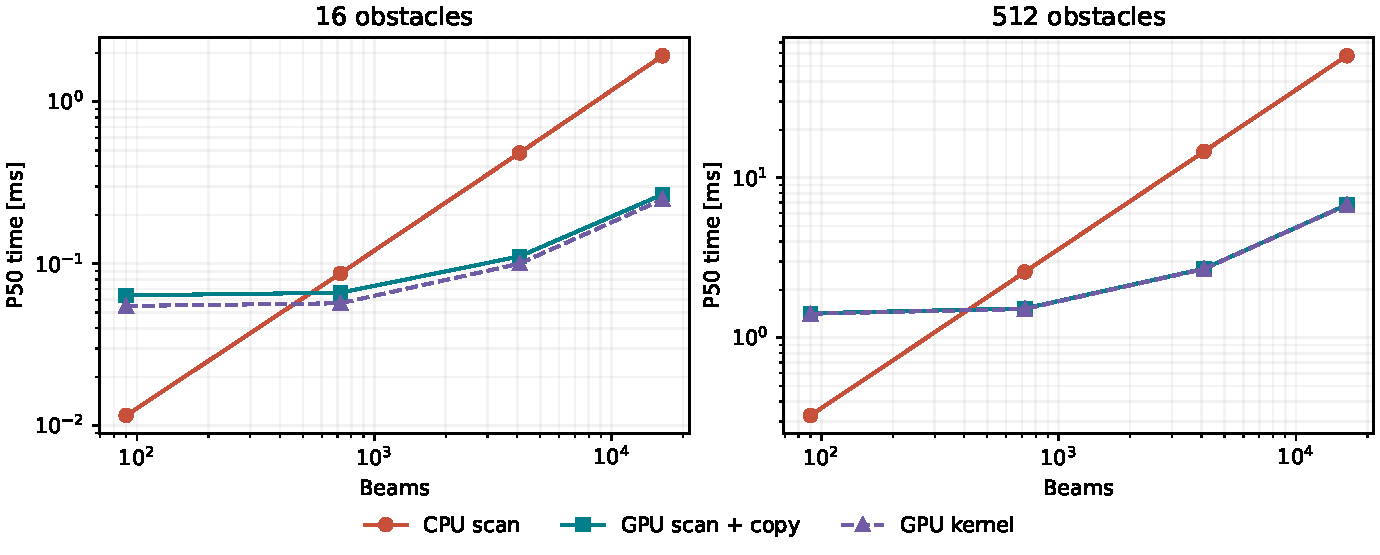
\includegraphics[width=\linewidth]{figures/ch20_cuda.pdf}
\caption{RTX 5060 主机实测，两个坐标轴都用对数。
驻留 GPU 扫描包含内核启动、同步和结果回传；虚线只表示内核，不能替代整条曲线。}
\end{figure}

\begin{center}\small
\begin{tabular}{rrrrr}\toprule
障碍/束 & CPU/ms & 内核/ms & 驻留扫描/ms & CPU/扫描\\\midrule
16/90 & 0.0116 & 0.0549 & 0.0638 & 0.18\\
16/720 & 0.0873 & 0.0571 & 0.0663 & 1.32\\
16/16384 & 1.923 & 0.250 & 0.267 & 7.19\\
512/90 & 0.327 & 1.413 & 1.422 & 0.23\\
512/16384 & 57.913 & 6.766 & 6.784 & 8.54\\\bottomrule
\end{tabular}
\end{center}
表中均为预热后的 P50。少量束时 GPU 明显更慢：并行度不足、启动固定成本和 double 算术代价
可能超过并行收益。720 束、16 障碍只有约 1.32 倍驻留扫描收益，不能写成数量级加速。

一次 setup 包括主机打包、分配、上传和事件创建；首组约 61 ms，还可能包含上下文初始化。
之后的 setup 约 0.029--0.110 ms；单独上传约 0.002--0.012 ms，不应每帧重复支付。
回传约 0.005--0.013 ms，已包含在驻留扫描里；不能把三个独立分位数相加当作总时长分位数。
CUDA 事件测内核，墙钟测同步后的回传和整次扫描；只量异步 launch 的返回时间会严重低估成本。

本次 16 组输出的 float 距离最大差为 0，随机位姿与噪声检查也通过；
这不是所有场景位级一致的承诺，仍保留浮点容差及特殊值检查。
练习 ch20-1 补齐 ray-circle 根选择，并解释为什么增加障碍、但不增加束数，未必能让 GPU 获益。
完整 ROS 噪声、消息构建和发布成本仍需在节点中另测，不能由此表推断。

\appendix
\addtocontents{toc}{\protect\newpage}
\chapter{数学回查与数值检查}
\begin{notebox}
\textbf{用途}\quad 从一个小例子回查符号、推导和代码含义；可随正文按需阅读。\\
\textbf{小实验}\quad 写出二维点变换的雅可比，用中央差分检查每一列。
\end{notebox}
\section{向量与矩阵：把多条标量关系放在一起}
二维位置 $p=(x,y)^T$ 是一个列向量，$T$ 表示转置，即把行列互换。
矩阵乘法可以按行理解：每一行与输入向量作点积，得到一个输出分量。例如
\[
 A=\begin{bmatrix}2&1\\0&3\end{bmatrix},\quad
 p=\begin{bmatrix}1\\2\end{bmatrix},\quad
 Ap=\begin{bmatrix}2\cdot1+1\cdot2\\0\cdot1+3\cdot2\end{bmatrix}
 =\begin{bmatrix}4\\6\end{bmatrix}.
\]
也可按列理解：$Ap=p_1A_{:,1}+p_2A_{:,2}$，即按输入分量组合矩阵的列。
第 02 章旋转矩阵的两列正是旋转后的两个单位轴。
$m\times n$ 矩阵把 $n$ 个输入分量变成 $m$ 个输出分量；相乘前先检查内侧维度相同。

长度与点积分别为 $\|p\|=\sqrt{x^2+y^2}$、$p^Tq=xq_x+yq_y$。
若 $n$ 为单位方向，$n^Tp$ 就是 $p$ 在该方向的有符号投影。
第 08 章点到直线残差 $n^T(p-q)$、第 13 章半空间 $n^Tp\le b$ 都使用这一含义。

\section{坐标变换与导数要使用同一种扰动}
位姿 $T_{AB}=(R,t)$ 把 B 系的坐标写成 A 系坐标：
\[
 p_A=Rp_B+t,\qquad
 R(\psi)=\begin{bmatrix}\cos\psi&-\sin\psi\\\sin\psi&\cos\psi\end{bmatrix}.
\]
由两列单位轴正交，$R^TR=I$。把 $t$ 移到左边，再左乘 $R^T$，得到逆变换
$p_B=R^T(p_A-t)$；因此逆位姿为 $(R^T,-R^Tt)$。
两次变换则直接代入：
\[
 p_A=R_{AB}(R_{BC}p_C+t_{BC})+t_{AB}
      =(R_{AB}R_{BC})p_C+R_{AB}t_{BC}+t_{AB}.
\]
这给出 \code{compose} 的旋转与平移两部分。
对\textbf{固定的}坐标变换求时间导数，平移常量消失，故 $v_A=Rv_B$、$a_A=Ra_B$。
若 $R,t$ 随时间变化，则应按乘积法则加入 $\dot R p_B$ 和 $\dot t$ 等项。
第 19 章在一次规划中固定 map/odom 变换，正是为了使用固定变换公式。

\subsection{雅可比的每一列在问什么}
对于向量函数 $f(x)$，逐个改变输入分量，记
\[
 J_{ij}=\frac{\partial f_i}{\partial x_j},\qquad
 f(x+\Delta x)\approx f(x)+J\Delta x.
\]
这是把单变量的一阶近似应用到每个输出分量。
第 $j$ 列表示只改变第 $j$ 个输入时，所有输出如何变化。
导数 $J_{ij}$ 的单位为“输出 $i$ 的单位/输入 $j$ 的单位”。

令 $p_B=(x,y)$，输入为 A 系平移与 yaw 的直接加法 $(t_x,t_y,\psi)$。
先展开输出，再分别求偏导：
\[
 p_{A,x}=t_x+x\cos\psi-y\sin\psi,\qquad
 p_{A,y}=t_y+x\sin\psi+y\cos\psi,
\]
\[
 J=\frac{\partial p_A}{\partial(t_x,t_y,\psi)}=
 \begin{bmatrix}1&0&-x\sin\psi-y\cos\psi\\
 0&1&x\cos\psi-y\sin\psi\end{bmatrix}.
\]
前两列表示平移 1 m 使对应坐标增加 1 m；最后一列为 m/rad。
在 $p_B=(2,-1)$、$\psi=0$ 时，第三列是 $(1,2)^T$；
yaw 增加 0.01 rad，点约移动 $(0.01,0.02)$ m。
机体系平移要先乘 $R$ 才成为 A 系位移，所以采用机体系扰动时，前两列相应变为 $R$。
明确“怎样改变输入”，才能选择相符的雅可比。

\subsection{梯度与反向传播就是链式法则}
标量代价 $L(f)$ 对向量 $f$ 的各偏导组成列向量 $\nabla_fL$。
小变化满足 $\Delta L\approx(\nabla_fL)^T\Delta f$。
代入 $\Delta f\approx J\Delta x$ 得到
\[
 \Delta L\approx(\nabla_fL)^TJ\Delta x
    =(J^T\nabla_fL)^T\Delta x,\qquad
 \nabla_xL=J^T\nabla_fL.
\]
这就是第 04、15、16 章反向传播的基本公式。
例如 $f=(x_1^2,x_1+x_2)^T$、$L=(f_1^2+f_2^2)/2$，
在 $(x_1,x_2)=(1,2)$ 处有 $f=(1,3)$、
$J=\left[\begin{smallmatrix}2&0\\1&1\end{smallmatrix}\right]$，
故 $\nabla_xL=J^Tf=(5,3)^T$。把 $L$ 直接展开再求导也得到同样结果。

\section{最小二乘：怎样综合不完全一致的测量}
两次位置测量分别为 $z_1=1.0$ m、$z_2=1.4$ m，标准差为
$\sigma_1=0.1$ m、$\sigma_2=0.2$ m。误差除以自己的标准差后再平方，得到无量纲代价
\[
 L(x)=\frac{(x-z_1)^2}{\sigma_1^2}+\frac{(x-z_2)^2}{\sigma_2^2}.
\]
相同距离误差对更精确的测量更严重，因此它得到更大权重。
令导数 $2\sum_i(x-z_i)/\sigma_i^2=0$，得到
\[
 x=\frac{z_1/\sigma_1^2+z_2/\sigma_2^2}{1/\sigma_1^2+1/\sigma_2^2}
   =\frac{100\cdot1.0+25\cdot1.4}{125}=1.08\ \mathrm m.
\]
结果更靠近标准差较小的第一条测量。该解对应加权平均。

\subsection{从标量求导到正规方程}
多维线性测量写为 $z=Hx+\epsilon$，残差 $r=Hx-z$。
令权重矩阵 $W$ 对称，目标为 $L=r^TWr$。
对 $x$ 加上 $\Delta x$，展开并收集一次项：
\[
 L(x+\Delta x)=L(x)+2\Delta x^TH^TWr+\Delta x^TH^TWH\Delta x.
\]
因此梯度为 $2H^TWr$，令其为零即
\[
 (H^TWH)x=H^TWz.
\]
独立测量时 $W$ 的对角元为 $1/\sigma_i^2$；存在相关误差时，使用协方差的逆 $W=\Sigma^{-1}$。
若 $\Sigma=CC^T$ 为三角分解，则
\[
 r^T\Sigma^{-1}r=(C^{-1}r)^T(C^{-1}r)=\|C^{-1}r\|^2.
\]
通过解三角方程 $Ce=r$ 得到白化残差 $e$，然后最小化它的普通平方和。
独立测量下 $C$ 的对角元为标准差，这恰好退化为前面的“除以标准差”。

求正规方程时，代码通过分解与回代求解，例如 Eigen 的 \code{ldlt().solve(rhs)}。
第 08 章演示三元方程的消元；第 16 章将同样思路用于轨迹块矩阵。
若某个非零方向 $d$ 满足 $Hd=0$，则 $H(x+\alpha d)=Hx$，代价沿该方向不变，
测量无法决定它。第 08 章走廊退化和第 10 章固定首帧，正是在处理这种自由方向。

\section{协方差：误差沿哪些方向一起变化}
设随机误差向量 $e=x-\mathbb E[x]$，其均值为零。
期望 $\mathbb E$ 表示同一实验重复很多次后的平均。定义
\[
 P=\mathbb E[ee^T],\qquad P_{ij}=\mathbb E[e_i e_j].
\]
对角元是每个分量的方差；非对角元为正，表示两误差常同号，为负则常反号。
每项单位是对应两个分量的单位相乘，例如位置/角度项为 m$\cdot$rad。
对任意方向系数 $a$，标量误差 $a^Te$ 的方差为
\[
 \mathbb E[(a^Te)^2]=a^T\mathbb E[ee^T]a=a^TPa.
\]
例如两位置误差的协方差为
$P=\left[\begin{smallmatrix}.04&.01\\.01&.09\end{smallmatrix}\right]\ \mathrm{m^2}$，
$e_1+2e_2$ 的方差为 $.04+4(.09)+4(.01)=.44\ \mathrm{m^2}$。
交叉项体现两误差共同变化的影响。

\subsection{传播公式来自直接展开}
若新误差近似为 $e'=Fe+w$，其中 $w$ 零均值、与 $e$ 独立，且协方差为 $Q$，则
\begin{align*}
 \mathbb E[e'e'^T]
 &=F\mathbb E[ee^T]F^T+F\mathbb E[ew^T]+\mathbb E[we^T]F^T+\mathbb E[ww^T]\\
 &=FPF^T+Q.
\end{align*}
中间两项因独立且零均值而为零。
非线性模型先作一阶近似，$F$ 便是当前点的状态雅可比。
观测残差同理得到 $S=HP^-H^T+R$；上标负号表示测量校正前的预测协方差。
第 09 章进一步用 $S$ 计算校正增益。

\section{中央差分：拿函数本身检查导数}
对单变量函数，在 $x$ 的两侧展开泰勒公式：
\begin{align*}
 f(x+h)&=f(x)+hf'(x)+\tfrac12h^2f''(x)+\tfrac16h^3f'''(x)+\cdots,\\
 f(x-h)&=f(x)-hf'(x)+\tfrac12h^2f''(x)-\tfrac16h^3f'''(x)+\cdots.
\end{align*}
两式相减再除以 $2h$，偶次项抵消，得到
\[
 \frac{f(x+h)-f(x-h)}{2h}=f'(x)+\tfrac16h^2f'''(x)+\cdots.
\]
在光滑函数附近，主要截断误差随 $h^2$ 缩小。
例如 $f(x)=x^3,x=1$，差分恰为 $3+h^2$，$h=0.3$ 时为 3.09，$h=0.1$ 时为 3.01。

\begin{center}\begin{minipage}{\linewidth}\makeatletter\def\@captype{figure}\makeatother
\centering
\begin{tikzpicture}
\begin{axis}[width=.72\linewidth,height=5cm,xmin=.45,xmax=1.55,ymin=0,ymax=3.6,
 xlabel={$x$},ylabel={$f$},grid=major,legend style={at={(1.04,.95)},anchor=north west,font=\small},
 tick label style={font=\small}]
\addplot[tealblue,thick,domain=.5:1.5,samples=80]{x^3};\addlegendentry{$x^3$}
\addplot[navy,dashed,domain=.7:1.5]{3*x-2};\addlegendentry{切线}
\addplot[orange!80!black,domain=.7:1.3]{3.09*x-1.82};\addlegendentry{两侧割线}
\addplot[only marks,orange!80!black] coordinates {(.7,.343)(1.3,2.197)};
\addplot[only marks,navy] coordinates {(1,1)};
\end{axis}
\end{tikzpicture}
\caption{中央差分取两侧点的割线斜率。缩小两侧间隔后，割线斜率趋向中间点的切线斜率。}
\end{minipage}\end{center}

计算机还带来舍入误差。若两次函数值的计算各带有大小约为 $\varepsilon$ 的误差，
相减再除以 $2h$ 后，误差可能达到约 $\varepsilon/h$。
因此缩小 $h$ 同时减小截断误差、放大舍入影响；应扫描多个步长，观察中间一段稳定区域。
向量函数按列重复同样操作：
\[
 J_{:,i}\approx\frac{f(x+h_i e_i)-f(x-h_i e_i)}{2h_i},
\]
$e_i$ 是第 $i$ 个单位坐标向量，$h_i$ 使用该输入的单位。
位置用米、角度用弧度分别扰动；差分与解析导数必须作用在同一个函数及同一种扰动上。

\begin{lstlisting}[language=bash,numbers=none]
mkdir -p tmp
c++ -std=c++17 -I/usr/include/eigen3 \
  -I exercises/appA/starter exercises/appA/check_jacobian.cpp \
  -o tmp/appA-check
./tmp/appA-check
\end{lstlisting}
练习 appA-1 使用点 $(2,-1)$ m、位姿 $(0.3,-0.8,0.7)$。
程序逐列建立正负扰动，比较两矩阵对应元素误差平方和的平方根。
在本例的单位与数值尺度下，$h=10^{-5}$ 时要求此范数小于 $10^{-7}$。
先用零角度的手算雅可比检查方向，再运行四个步长，可以同时检查坐标含义和导数实现。

\section{凸集与正定二次型为何适合规划}
凸集要求任意两点 $p,q$ 的连线 $(1-\lambda)p+\lambda q$ 仍在集合中，$0\le\lambda\le1$。
若 $Ap\le b,Aq\le b$，则逐行有
\[
 A[(1-\lambda)p+\lambda q]=(1-\lambda)Ap+\lambda Aq\le b.
\]
因此线性半空间的交集是凸集。把两点推广为非负权重和为 1 的多个点，仍有同样不等式，
这便是第 16 章 Bézier 控制点界的基础。

对称矩阵 $P$ 若对所有非零 $x$ 满足 $x^TPx>0$，称为正定；只要求非负则称为半正定。
例如
\[
 x^T\begin{bmatrix}2&1\\1&2\end{bmatrix}x
   =x_1^2+x_2^2+(x_1+x_2)^2>0\quad(x\ne0).
\]
而 $P=\operatorname{diag}(1,0)$ 只惩罚 $x_1$，允许沿 $x_2$ 的零方向。
对二次目标 $L=\tfrac12x^TPx+q^Tx$，若 $Px_*+q=0$，展开得到
\[
 L(x_*+d)-L(x_*)=\tfrac12d^TPd.
\]
$P$ 正定时，任何非零偏移都会使代价增加，从而得到唯一极小值。
第 18 章加入正定输入权重，使凝聚 QP 的二次矩阵具有这一性质。

\begin{center}\small
\begin{tabular}{lll}\toprule
要回查的量 & 关键问题 & 课程位置\\\midrule
位姿与速度 & 坐标变换固定还是随时间变化？ & 02、07、19\\
力、质量与加速度 & 输入与输出的单位是什么？ & 04、17\\
白噪声与偏置 & 独立采样还是持久累积？ & 06、09、附录 C\\
雅可比与梯度 & 输入怎样扰动，链式法则怎样连接？ & 08--10、15--16\\
ESDF 与走廊 & 距离代价与区域界怎样配合？ & 12--16\\
QP 约束 & 约束覆盖节点还是整段运动？ & 18\\\bottomrule
\end{tabular}
\end{center}
\paragraph{练习}
补全点变换雅可比并扫描差分步长；手算本附录的加权平均、梯度反传和协方差投影。
最后选一个正文函数，写出输入、输出、单位与一个可手算的特殊情形，再与源码对照。

\chapter{差速扫地机器人：先约束运动方向}
\begin{notebox}
\textbf{目标}\quad 从左右轮速得到圆心位姿，理解不能横移的含义。\\
\textbf{范围}\quad 独立无滑移运动学实验；主线仍为全向圆盘，未接入轮力矩或 NMPC。
\end{notebox}
\section{圆盘外形相同，能做的动作不同}
若希望先学建图与轨迹优化，全向圆盘能把问题分开；若研究扫地机器人，差速模型更贴近驱动约束。
圆盘半径仍负责碰撞，车轮半径 $r_w$ 和左右接地点间距 $b$ 则负责运动换算，三者不要混用。
轮速 $w_L,w_R$ 单位为 rad/s，同号为前进，理想无滑移模型为
\begin{equation}
 v=\frac{r_w(w_R+w_L)}2,\quad
 \omega=\frac{r_w(w_R-w_L)}b,\qquad
 \dot x=v\cos\psi,\quad\dot y=v\sin\psi,\quad\dot\psi=\omega.
\end{equation}
横向速度满足 $-\sin\psi\,\dot x+\cos\psi\,\dot y=0$。
它约束瞬时速度，不能写成一个简单的位置等式消掉；因此称为非完整约束。
机器人可以通过前进和转向改变横向位置，但不能直接侧移。

\lstinputlisting[language=C++,linerange={differential_kinematics_begin-differential_kinematics_end},
 includerangemarker=false]{../ros2_ws/src/motion2d/src/sim/differential_drive.cpp}
stepDifferential 复用第 04 章恒定机体系速度的精确 SE(2) 积分，避免另写一套近似积分器。
本函数没有电机、轮胎滑移或质量；阶跃轮速也不能凭空生成物理正确的瞬时 IMU 加速度。

\section{手算一次圆弧}
取 $r_w=0.05$ m、$b=0.4$ m、$w_L=2$、$w_R=6$ rad/s，
得到 $v=0.2$ m/s、$\omega=0.5$ rad/s、转弯半径 $v/\omega=0.4$ m。
从原点、yaw=0 出发，$t=\pi$ s 时应到达 $(0.4,0.4)$ m、yaw=$\pi/2$；
$t=4\pi$ s 恰好一圈。速度初始样本为施加轮速前的静止状态，随后为保持命令的运动学状态。

\clearpage
\begin{lstlisting}[language=bash]
ros2 run motion2d differential_drive_demo > textbook/data/appB_circle.csv
/usr/bin/python3 scripts/plot_appB.py
\end{lstlisting}
\begin{figure}[!ht]
\centering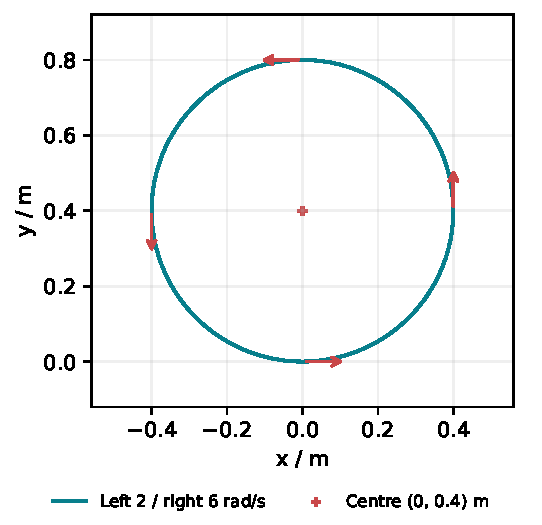
\includegraphics[width=.69\linewidth]{figures/appB_circle.pdf}
\caption{实际积分得到的圆弧，坐标等比例；箭头表示朝向，始终与运动方向相切。
这是独立几何实验，不包含障碍、轮动力学或 ROS 轨迹跟踪。}
\end{figure}

\section{怎样接到轨迹与控制}
对非零、正向运动的平滑参考 $p(t)$，可从速度与加速度计算
\begin{equation}
 \psi=\operatorname{atan2}(v_y,v_x),\qquad v=\|\dot p\|,\qquad
 \omega=\frac{v_xa_y-v_ya_x}{v_x^2+v_y^2},\qquad \kappa=\omega/v.
\end{equation}
此时 yaw 不能再独立任意指定。低速处上述分母接近零，停点和倒车必须定义单独的运动模式；
不能靠一个很小的分母下限，把不一致轨迹变成“可行”。原地旋转则应使用 $v=0$、左右反向轮速。

第 18 章预测矩阵是全向受力模型，直接换话题名不会变成差速控制。
一种扩展是以 $(x,y,\psi)$ 为状态、$(v,\omega)$ 为输入做 NMPC：在每次滚动优化中保留
三角函数运动方程，加入轮速及变化率限制，并在求解失败时制动。
若输入轮力矩，还应增加轮惯量、质量和轮地接触模型；这些扩展本课程未实现。

\paragraph{练习与验收}
appB-1 补全逆运动学，手算直行、倒车、原地转动与圆弧四组轮速。
核心测试另外检查四分之一圆解析解、分步积分一致性和零侧向速度。
改变两轮速的公共倍率，解释为何圆半径不变、转完一圈所需时间改变。

\chapter{进阶感知：理解随时间积累的误差}
\begin{notebox}
\textbf{目标}\quad 区分白噪声与持久偏置，推导随机游走的步长与方差，用独立重复试验检查模型。\\
\textbf{实验}\quad 单轴偏置工具可独立运行；后半部分提供延迟、逐束畸变与复杂环境的扩展练习。
\end{notebox}
\section{每次重新抽样，与保留上一次状态}
第 06 章每采样白噪声 $n_k$ 相互独立、均值为零、标准差为 $\sigma_n$。
若静止陀螺仪还带有缓慢变化的偏置 $b_k$，测量写为
\[
 y_k=y_k^{\rm ideal}+b_k+n_k.
\]
白噪声在下一次采样重新抽取；偏置则作为状态保存，在旧值上加一个小增量。
即使真实角速度为零，测量也可能在一段时间内持续偏向同一侧。
本附录使用最简单的零均值独立增量来模拟这种缓慢漂移：
\[
 b_{k+1}=b_k+\eta_k.
\]
先确定增量的方差如何随时间变化，再写代码生成它。

\section{为什么增量要乘时间间隔的平方根}
设 $b_0$ 已知，要求同样经过 $T$ 秒后，偏置分散程度与数值采样频率无关。
以 $\Delta t$ 为步长，共有 $K=T/\Delta t$ 个独立增量。
若每步方差为 $q(\Delta t)$，则
\[
 \operatorname{Var}(b_K-b_0)
 =\operatorname{Var}\left(\sum_{k=0}^{K-1}\eta_k\right)=Kq(\Delta t).
\]
希望总方差按 $\sigma_b^2T$ 增长，就应令
$Kq=\sigma_b^2T$，从而 $q(\Delta t)=\sigma_b^2\Delta t$。
标准正态样本 $\xi_k$ 的方差为 1，乘以一个数会让方差乘该数的平方，因此
\begin{equation}
 \eta_k=\sigma_b\sqrt{\Delta t}\,\xi_k,\qquad
 \xi_k\sim\mathcal N(0,1),\qquad
 b_{k+1}=b_k+\sigma_b\sqrt{\Delta t}\,\xi_k.
 \label{eq:bias_step}
\end{equation}
陀螺偏置 $b$ 单位为 rad/s；$\sigma_b$ 的单位为 $(\mathrm{rad/s})/\sqrt{\mathrm s}$，
乘 $\sqrt{\Delta t}$ 后恢复为偏置单位。
这与每次测量直接添加的 $\sigma_n$（rad/s）是两种参数。

取 $\sigma_b=0.002\ (\mathrm{rad/s})/\sqrt{\mathrm s}$，步长 0.01 s、单位样本 $\xi=1$，
增量为 0.0002 rad/s；步长改为 0.04 s，增量为 0.0004 rad/s。
固定 $T=10$ s 时，两种步长的方差都为 $0.002^2\times10=4\times10^{-5}\ (\mathrm{rad/s})^2$。
若误用 $\eta=\sigma_b\Delta t\xi$，则总方差变为
\[
 K\sigma_b^2\Delta t^2=\sigma_b^2T\Delta t,
\]
把采样率加倍便会错误地将总方差减半。

\lstinputlisting[language=C++,linerange={bias_walk_begin-bias_walk_end},
 includerangemarker=false]{../ros2_ws/src/motion2d/src/sim/bias_walk.cpp}
函数返回下一步偏置，由调用方保存；\code{unit_noise} 是调用方抽取的标准正态样本。
把随机数留在函数外，便于先用 $\xi=1$ 检查缩放，再用随机序列检查统计量。
六轴分别保存各自偏置，使用独立增量；偏置和测量白噪声也各用独立随机流。
重放时同时恢复初始偏置、引擎与分布对象状态，其中正态分布实现可能缓存一个待使用的样本。

\section{相邻偏置为什么相关}
取零初值，$b_j=\eta_0+\cdots+\eta_{j-1}$。
对 $k\ge j$，可写 $b_k=b_j+\eta_j+\cdots+\eta_{k-1}$，后面的增量与 $b_j$ 独立，故
\[
 \operatorname{Cov}(b_j,b_k)=\mathbb E[b_jb_k]
 =\mathbb E[b_j^2]=\sigma_b^2j\Delta t.
\]
用时间表示，就是 $\operatorname{Cov}(b(t),b(s))=\sigma_b^2\min(t,s)$。
两个时刻越晚，它们共享的历史增量越多，这正是偏置会持续一段时间的原因。
与之相比，独立白噪声在不同采样时刻的协方差为零。

\begin{lstlisting}[language=bash,numbers=none]
ros2 run motion2d bias_walk_demo tmp/appC_bias
# path.csv: one time history; summary.csv: independent trial endpoints
\end{lstlisting}
\begin{center}\begin{minipage}{\linewidth}\makeatletter\def\@captype{figure}\makeatother
\centering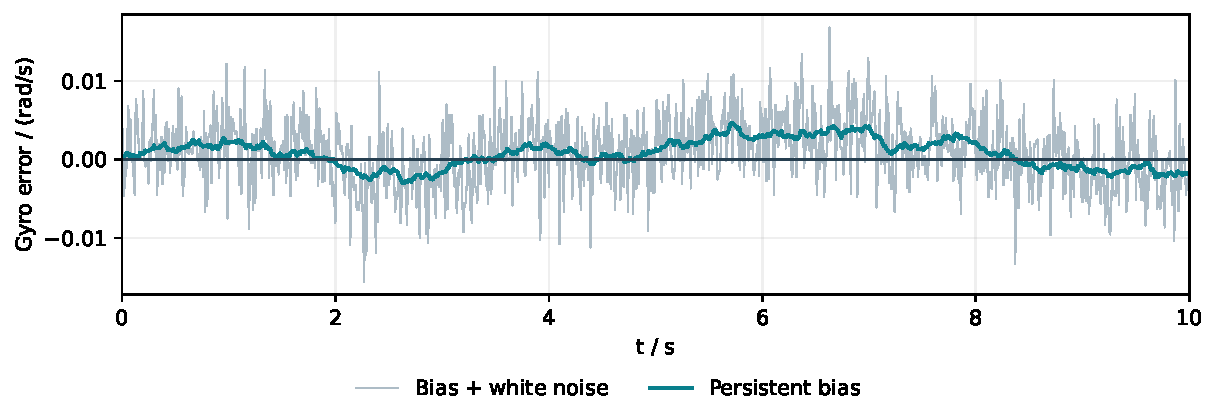
\includegraphics[width=\linewidth]{figures/appC_bias.pdf}
\caption{静止陀螺仪的一个单轴时间序列。深色是累积偏置，浅色在其上叠加每采样 0.004 rad/s 白噪声；短时抖动围绕当前偏置发生。}
\end{minipage}\end{center}
本图适合看误差随时间的形状。要估计“10 秒后偏置有多分散”，则从同一初值重复运行，
每次使用独立增量序列，只取各次的 10 秒终点。

\section{用许多终点估计方差}
记 $M$ 次试验终点为 $z_1,\ldots,z_M$，样本均值与样本方差为
\[
 \bar z=\frac1M\sum_i z_i,\qquad
 s^2=\frac1{M-1}\sum_i(z_i-\bar z)^2.
\]
为什么方差除以 $M-1$？设真实均值为 $\mu$、方差为 $V$。展开平方可得
\[
 \sum_i(z_i-\bar z)^2=\sum_i(z_i-\mu)^2-M(\bar z-\mu)^2.
\]
独立平均的方差为 $\operatorname{Var}(\bar z)=V/M$，两边取期望后右侧为
$MV-M(V/M)=(M-1)V$，所以除以 $M-1$ 后的期望恰为 $V$。
计算时还可展开为
\[
 s^2=\frac{\sum_i z_i^2-M\bar z^2}{M-1},
\]
这就是示例程序中 \code{sum}、\code{square} 和 \code{trials} 的关系。

\begin{center}\begin{minipage}{\linewidth}\makeatletter\def\@captype{figure}\makeatother
\centering
\begin{tikzpicture}[x=1cm,y=1cm,>=stealth,font=\small]
\draw[->,muted] (0,-1.2)--(6.5,-1.2) node[right]{$t$};
\draw[muted,dashed] (5.7,-1.1)--(5.7,1.6);
\draw[thick,tealblue] (0,0)--(1,.2)--(2,.1)--(3,.6)--(4,.4)--(5.7,1.2);
\draw[thick,navy] (0,0)--(1,-.2)--(2,-.1)--(3,-.5)--(4,-.8)--(5.7,-.6);
\draw[thick,orange!80!black] (0,0)--(1,.1)--(2,.3)--(3,.15)--(4,.4)--(5.7,.25);
\foreach \y/\lab in {1.2/z_1,.25/z_2,-.6/z_3}{\fill (5.7,\y) circle (.045) node[right]{$\lab$};}
\fill (0,0) circle (.04) node[left]{$b_0=0$};
\node[below] at (5.7,-1.2){$T$};
\node[anchor=west,align=left] at (7,.4){每次从零开始\\取同一时刻的终点\\计算均值与方差};
\end{tikzpicture}
\caption{独立试验终点的示意。每条折线使用不同增量序列；同一路径上各时刻共享历史，适合研究时间相关性。}
\end{minipage}\end{center}

示例取 $T=10$ s、$\sigma_b=0.002$，100 Hz 与 200 Hz 各运行 5000 次。
程序对每组频率使用固定种子，得到如下终点方差，单位均为 $(\mathrm{rad/s})^2$：
\begin{center}\begin{tabular}{lrr}\toprule
频率 & 理论方差 & 样本方差\\\midrule
100 Hz & $4.0000\times10^{-5}$ & $3.8782\times10^{-5}$\\
200 Hz & $4.0000\times10^{-5}$ & $3.9963\times10^{-5}$\\\bottomrule
\end{tabular}\end{center}
两组应围绕同一个理论值波动；改变频率后每条路径的具体形状可以不同。
将密度加倍，式\eqref{eq:bias_step}使增量加倍、终点方差变为四倍，
这是比观察某一条曲线“是否更抖”更直接的模型检查。

\section{偏置怎样变成角度漂移}
角速度误差积分为角度误差。先考虑固定偏置 $b_0$，则
$e_\psi(T)=\int_0^T b_0\,dt=b_0T$，随时间线性累积。
对于零初值的随机游走，均值仍为零，但角度方差包含各时刻偏置之间的相关性。
把积分看作许多小段相加，再用上一节的协方差公式，有
\begin{align*}
 \operatorname{Var}[e_\psi(T)]
 &=\int_0^T\int_0^T\operatorname{Cov}[b(u),b(v)]\,du\,dv\\
 &=2\sigma_b^2\int_0^T\left(\int_0^v u\,du\right)dv
 =\sigma_b^2\int_0^T v^2\,dv
 =\frac{\sigma_b^2T^3}{3}.
\end{align*}
第二行把正方形积分域分成 $u\le v$ 与 $u\ge v$ 两个对称三角形，前者的最小值为 $u$。
因此角度标准差为 $\sigma_bT^{3/2}/\sqrt3$。取本例参数，10 s 时约为 0.0365 rad。
这是步长趋小时随机游走积分的结果，适合与小步长数值实验比较。

每采样白噪声则按第 06 章给出角度方差 $\sigma_n^2T\Delta t$，因为各项独立。
固定偏置、缓慢偏置变化与独立测量噪声有不同的时间规律，滤波器应分别建模。
第 09 章偏置状态的过程协方差增量 $Q_b=\sigma_b^2\Delta t$ 正对应式\eqref{eq:bias_step}；
估计器还需要借助激光位姿约束，才能从运动观测中修正偏置。
若研究固定\emph{加速度}偏置 $b_a$，则速度误差为 $b_aT$，再次积分得到位置误差
$b_aT^2/2$；此时 $b_a$ 单位为 m/s$^2$，应与陀螺偏置分开计算。

\section{扩展传感器时，先画清时间与坐标}
基础雷达采用单时刻快照，基础 IMU 采用每采样白噪声。
可在独立实验验证后，依次把下面的变化接入传感器与估计接口。

\subsection{延迟改变到达时刻，保留采集时刻}
采集时刻 $t_s$ 的测量描述 $t_s$ 的状态，经过延迟 $\ell$ 后在 $t_a=t_s+\ell$ 到达。
例如一帧激光在 1.00 s 采集，1.08 s 到达；它应校正历史 1.00 s 状态，再按第 09 章缓存重传播。
若把 header 改成 1.08 s，就会把过去环境强行匹配到现在的位姿。
实现时可用按到达时间排序的队列保存消息，内部 header 保持原采集值。
先固定 80 ms 延迟，再增加乱序或丢包，分别观察历史缓存与缺测传播。

\subsection{逐束扫描需要逐束位姿}
旋转扫描中，第 $i$ 束在 $t_i=t_0+i\Delta t_b$ 采集。
设 $T(t_i)$ 把采集时刻的雷达坐标变到固定世界，单束局部点为
$p_i=(r_i\cos\theta_i,r_i\sin\theta_i)$。
先写成世界点 $q=T(t_i)p_i$，再变到选定参考时刻的雷达系：
\[
 p_{\rm ref}=T(t_{\rm ref})^{-1}T(t_i)p_i.
\]
例如雷达朝 x 正向匀速 1 m/s 平移，固定墙在世界 x=5 m。
取两个朝 x 正向的光束，0 s 的束测得 5 m，0.1 s 的束测得 4.9 m。统一到 0 s 时，第二束加回 0.1 m 位移，
两者都落在 5 m 的墙上。
仿真器用各采集时刻的真实状态生成量程，估计器用估计运动完成去畸变；
记录逐束时间后，才有依据区分快照、原始畸变点云和校正后点云。

\subsection{复杂环境会改变哪一层}
凹多边形首先改变几何查询：点是否在内部、圆盘扫掠是否碰撞、射线最近击中哪一条边。
可以画一个 U 形障碍，把凹口中的点作为自由点，再逐项对照这些查询结果。
第 03 章的随机凸多边形可作为基础对照。

动态障碍还增加时间维。例如一个圆心按 $c(t)=(1-t,0)$ 运动，半径 0.2 m；
先取半径为零的质点机器人静止在原点，当前净空为 0.8 m，1 s 后障碍却到达原点。
规划因此要比较对应时刻的机器人与障碍位置，而静态 ESDF 只描述一个时刻的几何。

全局重定位可以从“把机器人移动到远离上次估计的位置”开始实验。
先用当前局部 ICP 初值观察对应点为何匹配失败，再增加分散的候选位姿并逐个几何验证。
把候选搜索、局部优化和候选评分分别记录，有助于判断哪一步限制了恢复范围。

\section{练习：先预测，再用数据核对}
\begin{enumerate}
\item \textbf{代码 appC-1：}补齐随机游走步长；固定 $\xi=1$ 检查 $\Delta t$ 变四倍时增量的变化。
\item 从独立增量推导总方差与两个时刻的协方差；解释为何一条曲线上的样本不能替代独立终点。
\item 展开样本方差公式，手算三个终点 $(-0.01,0,0.01)$ rad/s 的均值与无偏方差。
\item 把密度加倍、总时间加倍，分别预测终点方差与积分角度方差的倍数，再做独立重复实验。
\item 用固定加速度偏置推导位置漂移 $b_aT^2/2$，与陀螺积分的单位逐项比较。
\item 按本章平移墙面例子手算两束去畸变；再设计一个固定延迟实验，标明采集、到达和校正时刻。
\end{enumerate}
练习与扩展实验说明见 \code{exercises/appC/README.md}。

\chapter{记录、回放与外部工具}
\begin{notebox}
\textbf{目标}\quad 保存一段传感器观测，关闭模拟器后重新生成里程计与地图；学会检查时间和输入一致性。\\
\textbf{先修}\quad 第 06、09、10 章；终端已加载主机 ROS 与课程工作空间。
\end{notebox}
\section{把一次运行变成可以反复使用的输入}
调试 SLAM 时，重新运动所产生的传感器序列可能因初值、运动或噪声而变化，难以判断结果变化来自参数还是输入。
rosbag2 把话题消息和时间存进文件；之后可将同一批扫描和 IMU 测量重新送给估计器。
这样调整匹配阈值或滤波噪声后，可以在相同观测上比较结果。

本实验只录制 \code{/scan} 与 \code{/imu/data_raw}。
估计里程计、map/odom 变换和地图由新运行的算法重新计算；传感器安装外参由回放 launch 提供。
如果同时播放旧估计的 TF，新旧两个算法会发布同一条变换边，显示和坐标查询便可能交替使用不同结果。
因此先画清“保存的输入”和“重新计算的输出”：
\begin{center}\begin{minipage}{\linewidth}\makeatletter\def\@captype{figure}\makeatother
\centering
\begin{tikzpicture}[>=stealth,font=\small,
 box/.style={draw=tealblue,fill=pale,rounded corners,minimum height=.85cm,align=center}]
\node[box,minimum width=2cm] (bag) at (0,0) {传感器 bag};
\node[box,minimum width=2.5cm] (player) at (4,0) {播放器};
\node[box,minimum width=3cm] (est) at (9,0) {雷达里程计与融合\\关键帧 SLAM};
\node[box,minimum width=3cm] (out) at (9,-2) {新里程计、TF\\观测地图与点云};
\draw[->] (bag)--(player);
\draw[->] (player)--node[above]{激光、IMU}(est);
\draw[->] (player.south)--++(0,-.85)-|node[pos=.25,below]{/clock}(est.south west);
\draw[->] (est)--(out);
\end{tikzpicture}
\caption{回放的数据流。文件提供固定观测，播放器提供仿真时钟，估计器从观测重新计算状态与地图。}
\end{minipage}\end{center}

\section{先区分采集、存储与墙钟时间}
一条消息涉及三种时刻：
\begin{center}\small
\begin{tabular}{lp{10cm}}\toprule
符号 & 含义与用途\\\midrule
$t_s$ & 消息 header.stamp 中的采集时间，决定测量对应哪个物理状态\\
$t_r$ & 录制器写入 bag 的接收/存储时间，播放器据此安排发送顺序\\
$w$ & 运行程序所经历的墙钟时间，用于观察播放速度与计算耗时\\\bottomrule
\end{tabular}
\end{center}
使用仿真时间录制时，$t_r$ 取录制器最近收到的 /clock 值；$t_s$ 则已在传感器消息中填写。
两个话题到达的先后可能不同，因此二者可相差一个时钟更新间隔。
例如消息的采集时间为 1.000 s，而录制器刚看到的时钟仍为 0.995 s，文件会保留这两个值。
估计器积分使用相邻 header 的差，存储时间用于重放调度。
具体选项可查阅 \href{https://github.com/ros2/rosbag2#simulation-time}{rosbag2 的仿真时间说明}，
并用本机 \code{ros2 bag record --help} 核对当前命令行。

\subsection{先录制一小段传感器}
按第 10 章启动仿真，保持暂停。在另一个终端启动录制器，再恢复仿真：
\begin{lstlisting}[language=bash,numbers=none]
# Terminal B; choose a fresh output directory.
ros2 bag record --use-sim-time -o tmp/my_sensors \
  --topics /scan /imu/data_raw
# Terminal C, after the recorder discovers both topics:
ros2 service call /sim/pause std_srvs/srv/SetBool "{data: false}"
\end{lstlisting}
录制数秒后在终端 B 按 Ctrl+C，让文件关闭；随后停止仿真与旧估计节点。
录制器收到第一个 /clock 后才开始写入消息，因此最初进入文件的采样可能晚于仿真零时刻。
用下面的命令检查文件实际包含的话题、条数和时间范围：
\begin{lstlisting}[language=bash,numbers=none]
ros2 bag info tmp/my_sensors
\end{lstlisting}
如果条数明显偏少，先检查录制器何时发现传感器、QoS 是否匹配，再检查发布频率。
消息内部的 frame、量程、协方差、噪声样本和采集时间均随消息保存。

\section{半速播放为什么仍用原来的积分步长}
在新的终端中启动只含估计节点的回放栈，再启动播放器：
\begin{lstlisting}[language=bash,numbers=none]
# Terminal A; this launch contains estimators and sensor extrinsics.
ros2 launch motion2d_bringup replay_slam.launch.py rviz:=true
# Terminal B; the simulator and old estimators have stopped.
ros2 bag play tmp/my_sensors --clock 200 --rate 0.5
\end{lstlisting}
播放器是这一回放系统的 /clock 发布者，估计节点均使用仿真时间。
设播放倍率为 $r>0$，文件中两条消息的存储时差为 $\Delta t_r$，
则计划的墙钟发送间隔为 $\Delta w=\Delta t_r/r$。
半速 $r=0.5$ 时，计算机有两倍墙钟时间处理同一段运动；消息内部 $t_s$ 保持原值。

例如陀螺测量为 0.2 rad/s，两条 IMU 采集时间相差 0.005 s，积分得到
\[
 \Delta\psi=\omega\Delta t_s=0.2\times0.005=0.001\ \mathrm{rad}.
\]
半速回放时，这两条消息可能相隔约 0.010 s 墙钟时间到达，角度增量仍为 0.001 rad。
若改用到达间隔积分，就会错误地将机器人转速或运动时长放大。

\begin{center}\begin{minipage}{\linewidth}\makeatletter\def\@captype{figure}\makeatother
\centering
\begin{tikzpicture}[x=1cm,y=1cm,>=stealth,font=\small]
\node[anchor=east] at (-.6,0){采集时刻 / s};
\node[anchor=east] at (-.6,-1.7){回放经过时间 / s};
\draw[->,muted] (0,0)--(8,0);\draw[->,muted] (0,-1.7)--(8,-1.7);
\foreach \x/\s/\w in {1/1.000/0,4/1.005/0.010,7/1.010/0.020}{
 \draw[dashed,linecolor] (\x,-.15)--(\x,-1.55);
 \fill[tealblue] (\x,0) circle (.05) node[above]{$\s$};
 \fill[navy] (\x,-1.7) circle (.05) node[below]{$\w$};
}
\node[fill=white,inner sep=3pt] at (4,-.85){同一条消息，header 保持原值};
\end{tikzpicture}
\caption{半速播放的时间对照。为突出比例，图中假设存储时差等于采集时差；实际回放发送顺序由文件时间决定。}
\end{minipage}\end{center}

\subsection{TF 每条边由谁计算}
回放 launch 复用雷达里程计、IMU 融合、估计里程计适配与关键帧 SLAM 四个节点。
雷达里程计提供扫描位姿，融合节点结合 IMU，适配器将融合结果转换为统一里程计接口。
TF 分工为：
\begin{center}\small
\begin{tabular}{ll}\toprule
变换边 & 发布者\\\midrule
map $\to$ odom & 关键帧 SLAM\\
odom $\to$ base\_link & 估计里程计适配器\\
base\_link $\to$ laser & 静态雷达外参发布器\\
base\_link $\to$ imu\_link & 静态 IMU 外参发布器\\\bottomrule
\end{tabular}
\end{center}
课程传感器与圆盘中心重合、朝向一致，所以两条外参是零平移、零旋转。
更换真实记录时，应填入标定的安装位姿，使扫描与惯性测量转换到正确机体系。
RViz 的 Fixed Frame 设为 map，观察新生成的占据地图、注册点云与估计轨迹。
若点云跟随错误的坐标移动，先检查 frame 名称和这四条边的时间，再调整 SLAM 参数。

\section{用自动实验追踪每一条输入}
在仓库根目录可运行完整录制与回放例子，输出路径应是新的目录：
\begin{lstlisting}[language=bash,numbers=none]
/usr/bin/python3 scripts/run_appD.py --output tmp/my_replay
\end{lstlisting}
脚本在独立 ROS 域内启动暂停的 reference 模型，等待录制器订阅两类传感器，推进至六秒后停止。
它关闭录制器和模拟器，再启动上述估计栈并半速回放。
场景采用 seed42 随机世界、720 束/10 Hz 激光和 200 Hz 白噪声 IMU，参数来自第 10 章。

\subsection{先比较字段，再解释结果}
本次记录中的每条传感器消息都有本话题内唯一的采集时间戳。脚本建立
“话题 $+$ 采集纳秒 $\to$ 字段摘要”的对应，用它配对现场接收、文件读取与回放接收的消息。
纳秒值为
\[
 t_{\rm ns}=10^9\,\text{sec}+\text{nanosec},
\]
保留整数能避免把纳秒转换成浮点秒后丢失末位。
字段摘要的核心是下面几行：
\lstinputlisting[language=Python,linerange={replay_digest_begin-replay_digest_end},includerangemarker=false]{../scripts/run_appD.py}
\code{message_to_ordereddict} 展开消息的每个字段，JSON 固定键顺序与分隔符，
SHA-256 把该表示变为便于比较的固定长度摘要。相同字段将产生相同摘要；发现不同摘要时，
再展开消息查找具体差异。量程中的 NaN、无回波、frame、stamp 和协方差都参与比较。

这样比较关注测量本身。CDR 序列化还可能插入用于对齐的填充字节，重新编码时填充值可以变化。
例如某个按 4 字节对齐的字段前已有 1 字节内容，就需补 3 字节以移动到下一个 4 字节边界。
这些填充用于存放布局，解码后的测量数值由真正字段决定。
因此检查传感器重放时，先解码再比较字段，可以排除填充差异的干扰。

\subsection{怎样读这次记录的统计量}
随教材保存的一组结果为：59 帧扫描、1180 帧 IMU，存储时间从 0.105 到 6.000 s，
存储与采集时刻最大相差 0.005 s。
初始时钟与订阅建立影响了文件起点，因此应以文件实际条数为准。
回放结束后，最后里程计时刻为 6.000 s，地图有 12556 个已观测格，累计点云有 537 点。
它们分别说明输入记录长度、估计处理进度以及地图是否已累积观测。
对应字段见 \code{textbook/data/appD_replay.json}。

先确认回放输入逐字段一致，再检查估计输出的完整性。
研究定位精度时，另保存独立的评价真值，按第 19 章做时间对齐并计算 ATE/RPE；
研究地图质量时，在已观测区域比较墙体位置、厚度与占据分类。
这种顺序有助于区分输入丢失、时间处理错误和算法估计误差。

\section{在同一记录上接入外部二维 SLAM}
选做对照可使用 \href{https://github.com/SteveMacenski/slam_toolbox#api}{slam\_toolbox 的官方接口说明}：
输入扫描与 odom 到 base 的有效变换，由算法输出地图。
先为目标版本整理输入表，写清扫描话题、外参、里程计来源和坐标名称。
如果一个系统直接融合 IMU，另一个通过融合里程计间接使用 IMU，应把这条信息路径写进比较条件。

对照时按如下顺序准备：
\begin{enumerate}
\item 固定同一份传感器 bag 与外参；确定每个算法可获得哪些观测和先验。
\item 串行运行两个系统，使每次只有一个发布者计算 map/odom；每次从新的算法状态开始。
\item 固定回放速率、初值和计算预算，保存参数、版本、状态及输出轨迹。
\item 用同一评价真值、时间交集与 ATE/RPE 定义比较；同时记录失败次数与地图质量。
\end{enumerate}
若某个系统获得更精确的里程计先验，结果就同时反映先验与算法的作用。
可先比较整套系统，再固定共同先验做第二组实验，逐步缩小影响因素。

\section{从教材找到函数说明，再回到代码}
教材按问题展开推导，API 文档按函数名和类型检索。
在仓库根目录运行
\begin{lstlisting}[language=bash,numbers=none]
bash scripts/build_api.sh
# Open tmp/doxygen/html/index.html in a browser.
\end{lstlisting}
脚本优先使用系统 Doxygen，也支持仓库 tmp 中准备好的局部工具。
若提示找不到 Doxygen，安装后重试；公式渲染使用主机 LaTeX 工具链。

以附录 C 的 \code{stepBiasWalk} 为例，先在 API 中找到声明，再对照这些字段：
\begin{center}\small
\begin{tabular}{lp{10cm}}\toprule
字段 & 阅读时要获得的信息\\\midrule
brief & 一次标量偏置更新，说明函数解决的问题\\
param & bias 是当前偏置；density 是偏置单位除以平方根秒；dt 是实际经过的秒数；unit\_noise 是标准正态样本\\
return & 下一步偏置，单位与输入 bias 相同，调用方将它保存到下一次采样\\
details / pre & 更新公式、独立样本要求，以及时间和密度的有效范围\\\bottomrule
\end{tabular}
\end{center}
随后到源文件找到式\eqref{eq:bias_step}，用 $\Delta t=0.01$ s、$\xi=1$ 手算一次调用。
最后打开偏置演示，查看随机数如何产生、返回值如何保存。
从“公式—声明—函数体—调用点”走一遍，就能看懂一个小模块怎样接入程序。

自己编写注释时，用输入的物理含义解释单位与前提。例如
“dt：实际经过的时间，单位 s”比单写“dt：时间”更有帮助。
数学可用 Doxygen 的行内或行间公式语法书写，再生成页面检查公式是否正确显示。

\section{把实验写成别人可以重做的步骤}
可复制仓库中的报告模板：
\begin{center}\code{docs/EXPERIMENT_REPORT_TEMPLATE.md}\end{center}
先提出一个能比较的问题，例如“偏置密度加倍后，10 秒终点方差是否变为四倍”。
写出模型预测，然后列出运行版本、参数、种子、时长与重复次数，提供生成原始数据的命令。
结果中同时保留每组样本数、成功或失败状态、统计指标与单位，读者便能重算你的结论。

性能实验按第 20 章分别记录准备、计算、传输和消息阶段，注明预热与计时边界；
轨迹实验按第 16--19 章说明空间检查、动力学界、时间对齐和跟踪指标。
当结果偏离预测时，先判断是输入、坐标、时间、数值误差还是模型条件发生了变化，
再有针对性地修改下一组实验。

\section{练习：重放同一段运动}
\begin{enumerate}
\item \textbf{代码 appD-1：}从混合话题列表中选出扫描与原始 IMU；缺少必要输入时说明缺失项。
\item 对 0.2 rad/s、采集间隔 0.005 s 的陀螺数据，分别求 0.5 倍和 2 倍播放时的墙钟间隔与角度增量。
\item 运行自动回放例子，读取 summary.json 和 bag 元数据，解释采集与存储时间的差异。
\item 将一条 IMU 的协方差改动一个元素，预测字段摘要是否改变；说明为何检查时包含协方差与 frame。
\item 画出回放 TF 树，标注每条边的发布者；更换传感器安装位置时应改哪两条边？
\item 在 API 中找到偏置函数，从声明追到调用点；复制报告模板，填写附录 C 的两频率比较。
\end{enumerate}
练习入口与手算提示见 \code{exercises/appD/README.md}。

\end{document}
